\section{Background, observations, and motivation}
\label{sec:dataset-analysis}

%\subsection{Layer size distribution}
%
%\subsection{File size distribution}
%
%\subsection{Redundant file distribution}

%\section{Deduplication performance analysis} % just find the problem and benefit
\label{sec:background}

%\paragraph{Deduplication for improving storage capacity.}

On-cloud global deduplication software is widely adopted by cloud enterprises for reducing cloud storage consumption and overall storage cost. 
For example, StorReduce~\cite{storReduce}, the deduplication software used by
Google cloud and AWS, 
performs in-line transparent data deduplication. 
%StorReduce resides between the client's application and the hosting cloud storage.
%A number of deduplication methods focus on client-side data deduplication to ensure that only unique files are uploaded, 
%to save network bandwidth, by having the client send a duplicate check request~\cite{xxx}~\cite{xxx}. 
%For example, xxxx\NZ{Hadeel, can you add one example and few relatedwork citation?}. 
Intuitively, such deduplication techniques can be leveraged to eliminate redundant data from the Docker image storage system.  
Except, the Docker image dataset is not amenable to deduplication 
as the images are \emph{compressed archival files}.
%Intuitively, registries can be deployed as a proxy cache to host frequently requested layers to speedup image pulls and improve performance 
%while the backend cloud storage can leverage deduplication to save storage space.
%However, there are several unique problems concerning the integration of caching and deduplication to the unique Docker registries workload: \textbf{compressed layers}. 
%We investigate the potential for data reduction in the Docker registry by estimating the efficacy of layer sharing and file-level deduplication.
%We noticed that the number of public repositories is constantly increasing with a growth that amounts 
%to around 1 million repositories annually. 
%This corresponds to~130\,TB of annual growth in storage needs 
%\HA{but it is actually less because of shared layers, right?}, 
%costing around~\$15,000 a month if Google Cloud Storage is used~\cite{GoogleCloudStoragePricing}.
%This growth implies significant benefits to data deduplication. 


As discussed in~\cref{sec:intro}, only $3$\% of the files in a sample Docker hub image collection were found to be unique, mainly becuase 
 compressed files have a very low deduplication ratio~\cite{meister2012study}.
Thus, 
we can realize significant space savings if we can remove the 
duplicate files. This entails decompressing files before performing deduplication, and collecting components of layers from multiple servers.
%
To quantify the performance overhead of such an approach involving decompressing, deduplication, and then re-compressing,
we setup five registry instances. Each instance has a local file system as their backend storage system. We
implemented file-level deduplication with decompression and compression operations.
We replayed the IBM registry workload \texttt{dal}~\cite{dockerworkload} 
%by sending requests randomly 
randomly to our five registries and measured the latency. 
%
Figure~\ref{fig:avg_latency_dedup_nodedup} shows the average latency observed 
across five registries.
%\arb{average across what??}\NZ{addressed}.
Note that since 
%the IBM registry workload 
\texttt{dal} does not contain real layers,
we extract the layer digest from each request and match it with a layer randomly selected from our Docker Hub dataset to emulate realistic requests.

Without deduplication,
the average latency for requesting a layer is about $2$~s for layers with sizes $\textless50$~MB.
The latency increases to $12$~s when the above deduplication is implemented in the backend storage system.
Furthermore, Docker registry performance drops down dramatically for larger layers.
We observe that the average latency for requesting layers $\textgreater50$~MB and $\textless1$~GB
is about $128$~s. The latency worsens with dedupliation to on average of about $800$~s.
%\NZ{todo:graph: less than, }
%\HA{running five registries, replaying dal trace using trace replayer-cite, and since the replayer doesn't use real layers we randomly match the request to our dataset downloaded from docker hub. describe how we got these numbers. for dedup, we simply implemented a decompress/compress + file-level deduplication on backend storage systems, we use a CHT based distributed storage system. Figure~\ref{fig:avg_latency_dedup_nodedup}}
\begin{figure}[t]
	\centering
	%\scriptsize
	\begin{minipage}{0.225\textwidth}
		\centering
		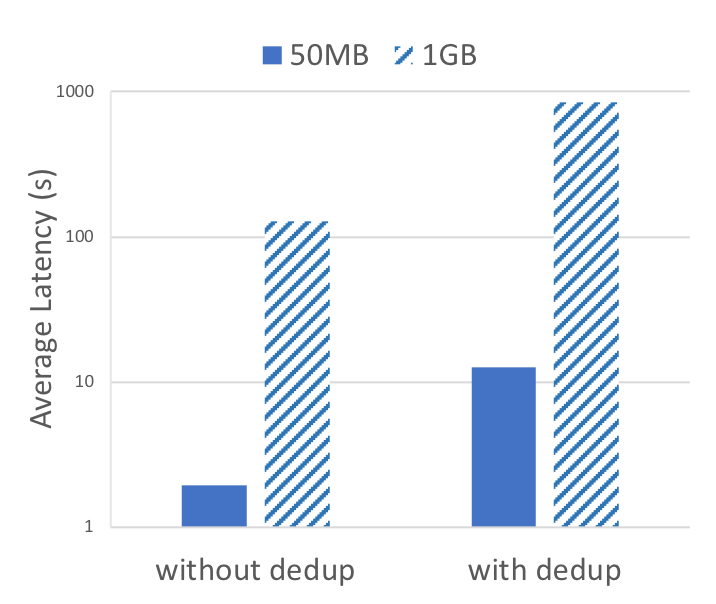
\includegraphics[width=1\textwidth]{graphs/avglatency_dedup_nodedup.png}
		\caption{Average latency.}
		\label{fig:avg_latency_dedup_nodedup}
	\end{minipage}
	\begin{minipage}{0.225\textwidth}
		\centering
		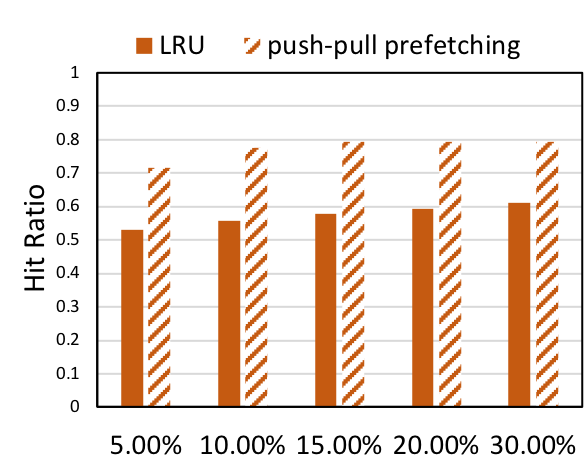
\includegraphics[width=1\textwidth]{graphs/lru_prefetch_hits.png}
		\caption{Hit ratio.}
		\vspace{-3pt}
		\label{fig:lru_prefetching_hits}
	\end{minipage}
\end{figure}
% for LRU and push-pull prefetching under different cache sizes (\% of total accessed layers).



%\begin{figure*}[t]
\centering
			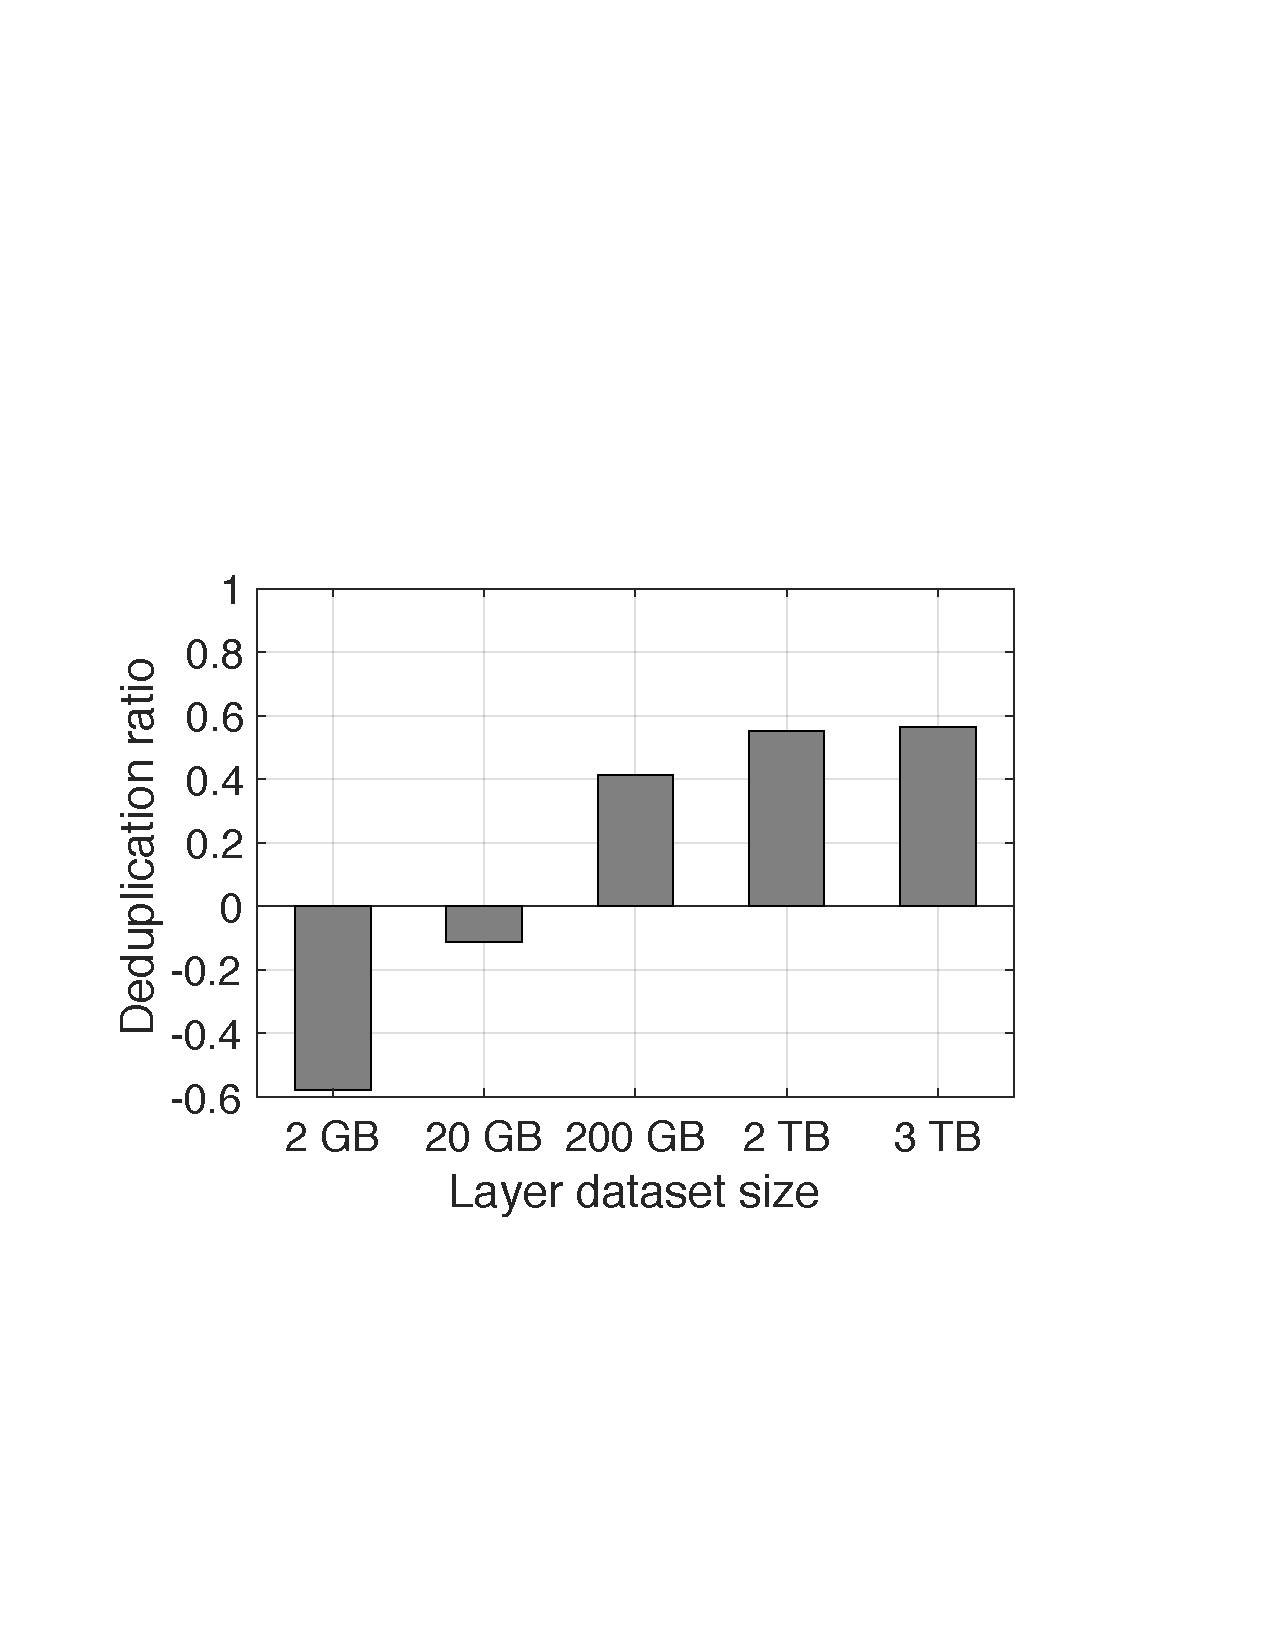
\includegraphics[width=0.2\textwidth]{graphs/dedup_vs_compression.pdf}
			\caption{Efficiency of deduplication over compression}
		%	\vspace{-3pt}
			\label{fig:cacheefficiency}

\end{figure*}

%\begin{figure}[t]
%	\centering
%	\begin{minipage}{0.26\textwidth}
%		\centering
%		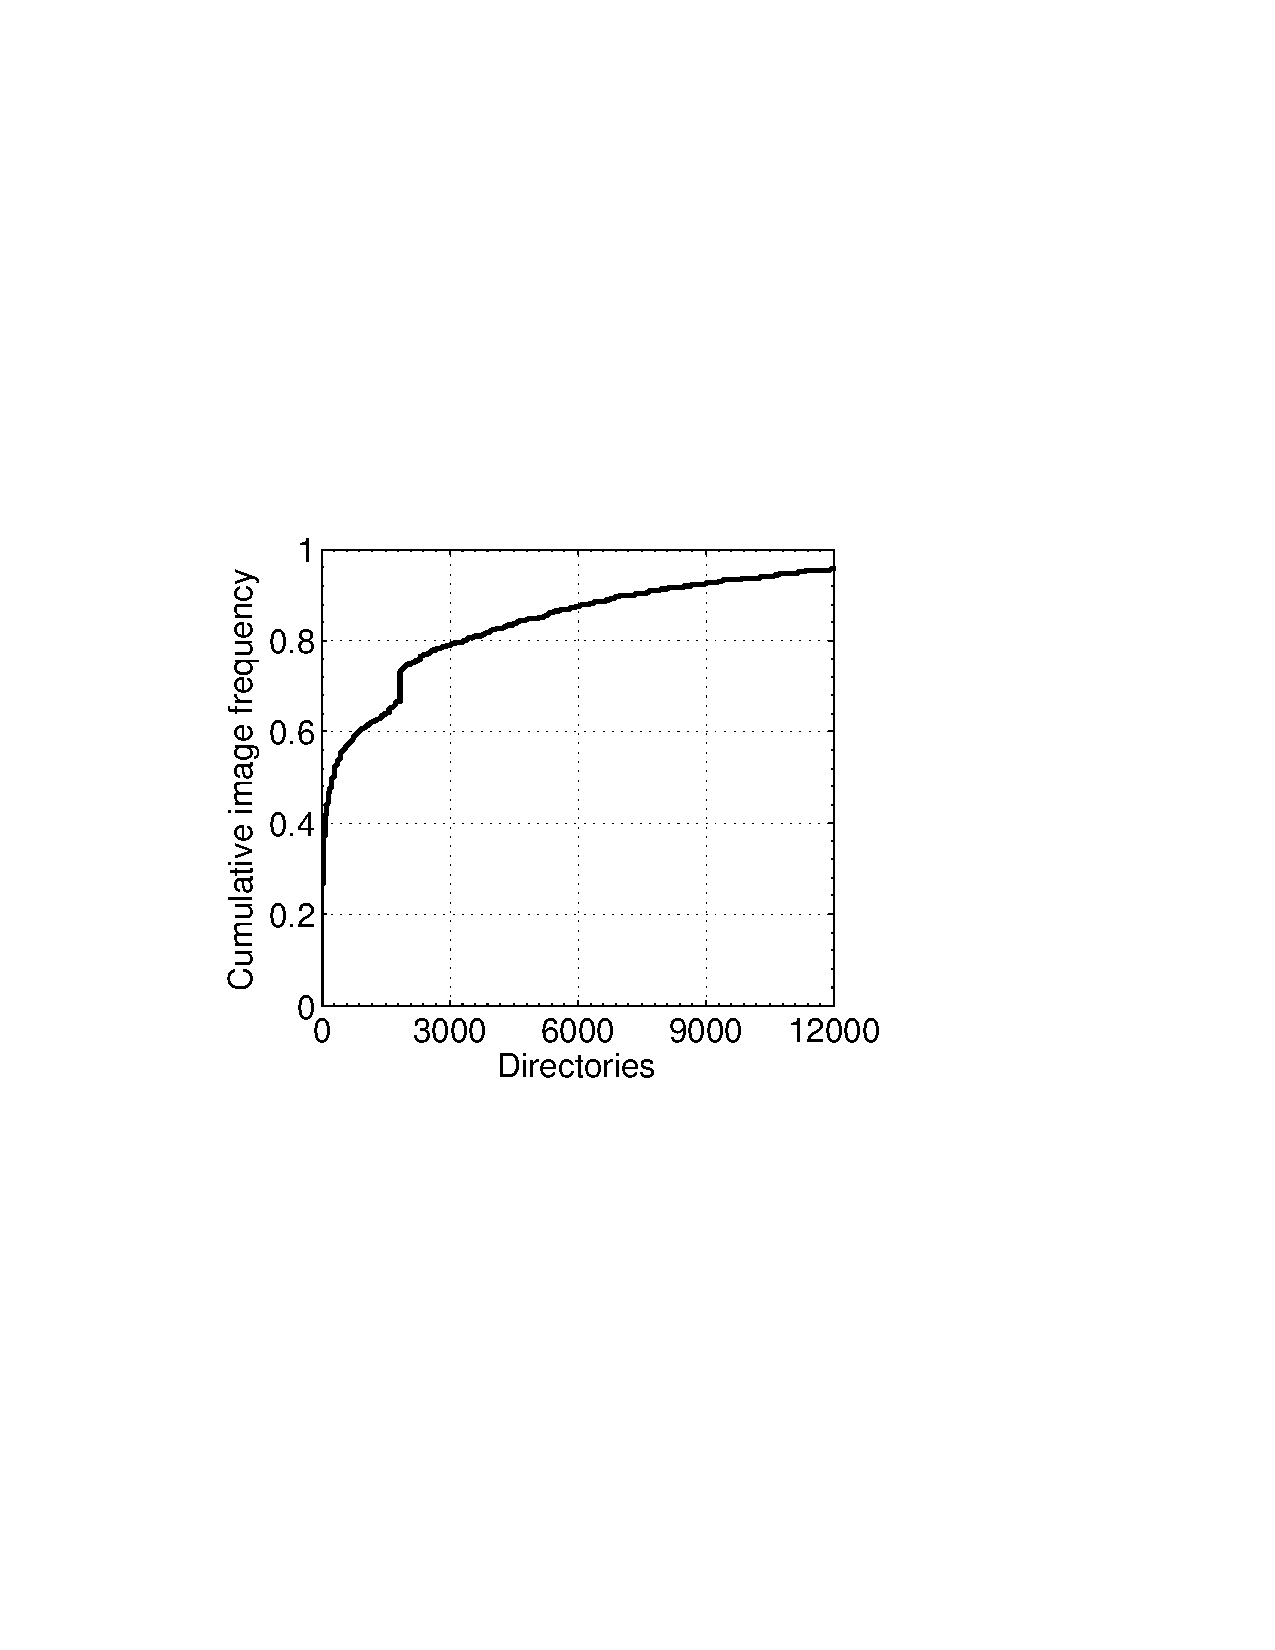
\includegraphics[width=1\textwidth]{graphs/dir.pdf}
%		\caption{CDF of images by\newline directories}
%		\label{fig-dir}
%	\end{minipage}%
%	\begin{minipage}{0.24\textwidth}
%		\centering
%		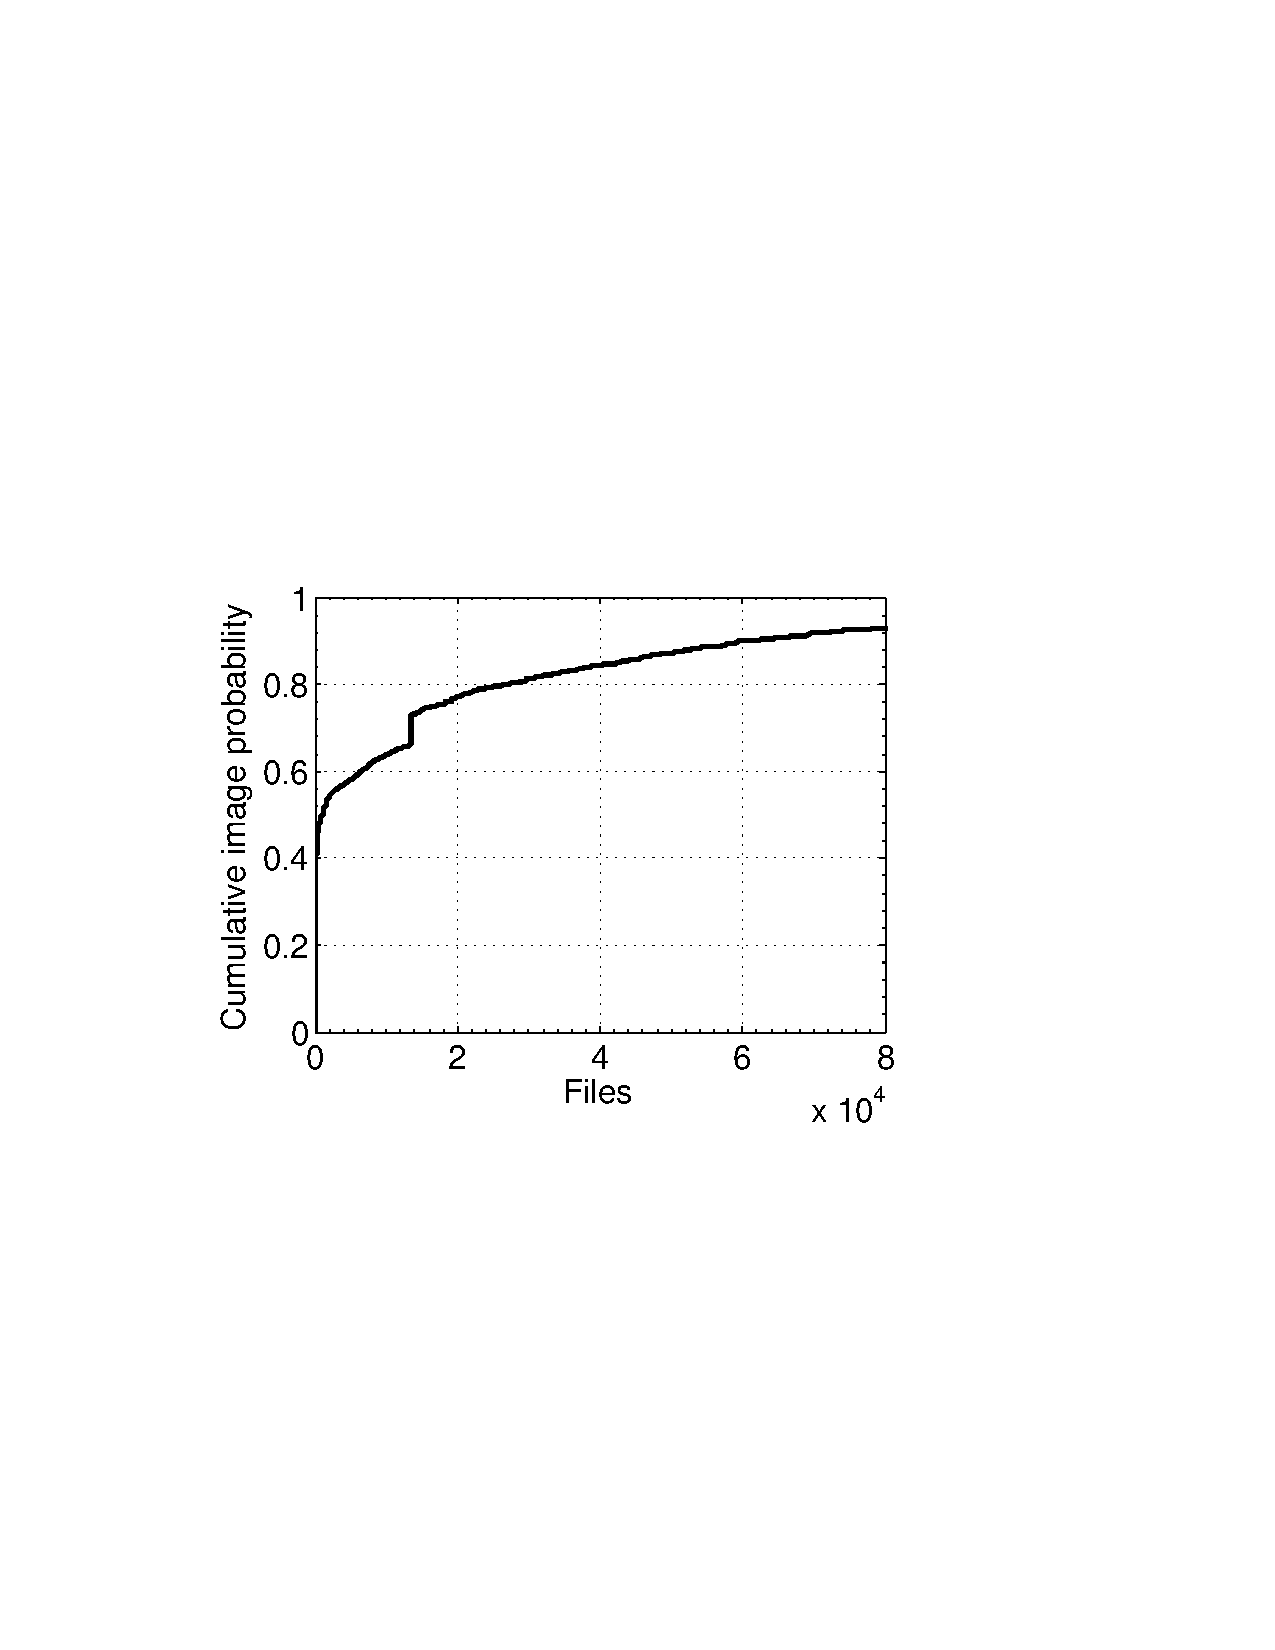
\includegraphics[width=1\textwidth]{graphs/file.pdf}
%		\caption{CDF of images by files}
%		\label{fig-file}
%	\end{minipage}
%\end{figure}

%\begin{figure}[htbp] 
%	\begin{minipage}{0.5\linewidth} 
%		\centering 
%		\includegraphics{circle} 
%		\caption{A Circle} 
%		\label{fig:circle} 
%	\end{minipage}% 
%	\begin{minipage}{0.5\linewidth} 
%		\centering 
%		\includegraphics{rectangle} 
%		\caption{A Rectangle} 
%		\label{fig:rectangle} 
%	\end{minipage} 
%\end{figure}

\subsection{Inter-layer deduplication}

\paragraph{Duplicated files shared among layers}
Although Docker uses COW file system to minimize redundant data inside each image and
 supports the sharing of layers among different images to remove redundant data in Docker registry backend storage system,
 a large amount of duplicated files are observed among layers within different images.  
According to the deduplication analysis on Docker Hub dataset~\cite{dedupanalysis},
only 3.2\% of files are unique, resulting in deduplication ratio of 2x in terms of capacity. 
These large amount of duplicated files %shared among different layers associated with different images
are mainly executables, object codes, libraries, and source codes probably
imported by different image developers using the same package installers or version control systems such as
\texttt{apt},  \texttt{pip} or \texttt{git} to install or get similar dependencies or source codes.
The file-level duplication among different layers cannot be \emph{deduplicated} 
by using layer-level content addressable storage system adopted by current registry.

\paragraph{Layer deduplication}
As containerization frameworks like Docker and Kubernetes keep gaining in popularity,
more applications are encapsulated into images, pushed into registry, and stored on Cloud.
By using \emph{R}-way replication, the amount of layers grows exponentially and will explode in future.
This is not just a requirement of more disks.
It goes beyond just hardware upgrade or even datacenter expansion,
and into large volumes of data management challenges, such as missive and slow data migration during scale-out or scale-up.
 
File-level deduplication can be implemented on registry by first decompressing the compressed layer tarballs and 
removing the duplicated files across different layers.
In this case, 
layer dataset stored on registry can be largely reduced for good data management.
However,  
\texttt{pulling}
a layer from registry requires restoring a layer,
which involves file fetching, layer archiving, and layer compression.
These extra operations incurs a considerable overhead especially for  
\texttt{pulling} layer performance which is crucial for container startups. 
Is it possible to deduplicate layers while maintaining a good layer \texttt{pulling} performance?
We analyze registry workloads and 
optimize the performance by exploring workload patterns and user access patterns.   
%Consider that deduplication incurs a performance overhead and the current Docker registry already stores layers in compressed format to save space and network transfer overhead. We first analyze the space efficiency of a registry that performs decompression and file-level deduplication and compare it to a registry that naively stores compressed layers.

%In Figure~\ref{fig:cacheefficiency}, the x-axis values correspond to the sizes of $5$ samples of registry data of varying sizes with traditional layer compression. For a traditional registry, the compressed layer tarballs will be kept as is.
%While a registry with file-level deduplication will store \emph{deduplicated} layers (i.e., unique files). 
%The y-axis shows how much space a registry with file-level deduplication can save over compressed layer tarballs.
%For the first two samples of the dataset, with size less than $20$~GB, 
%there is no benefit to \emph{deduplicate} layers because the deduplication ratio is very low.
%However, when the dataset size is $200$~GB and over, we can save over $40\%$ more space increasing almost linearly with the size of the layer dataset.
%This verifies the benefit of deduplicating layers as the registry size increases.
%Before describing Sift, we must understand the storage pressure and trends in the access patterns of the Docker registries at the layer and repository level.

\subsection{Predictable User Access}
%\begin{figure*}[t]
%		\begin{minipage}{0.32\linewidth}
%			\centering
%			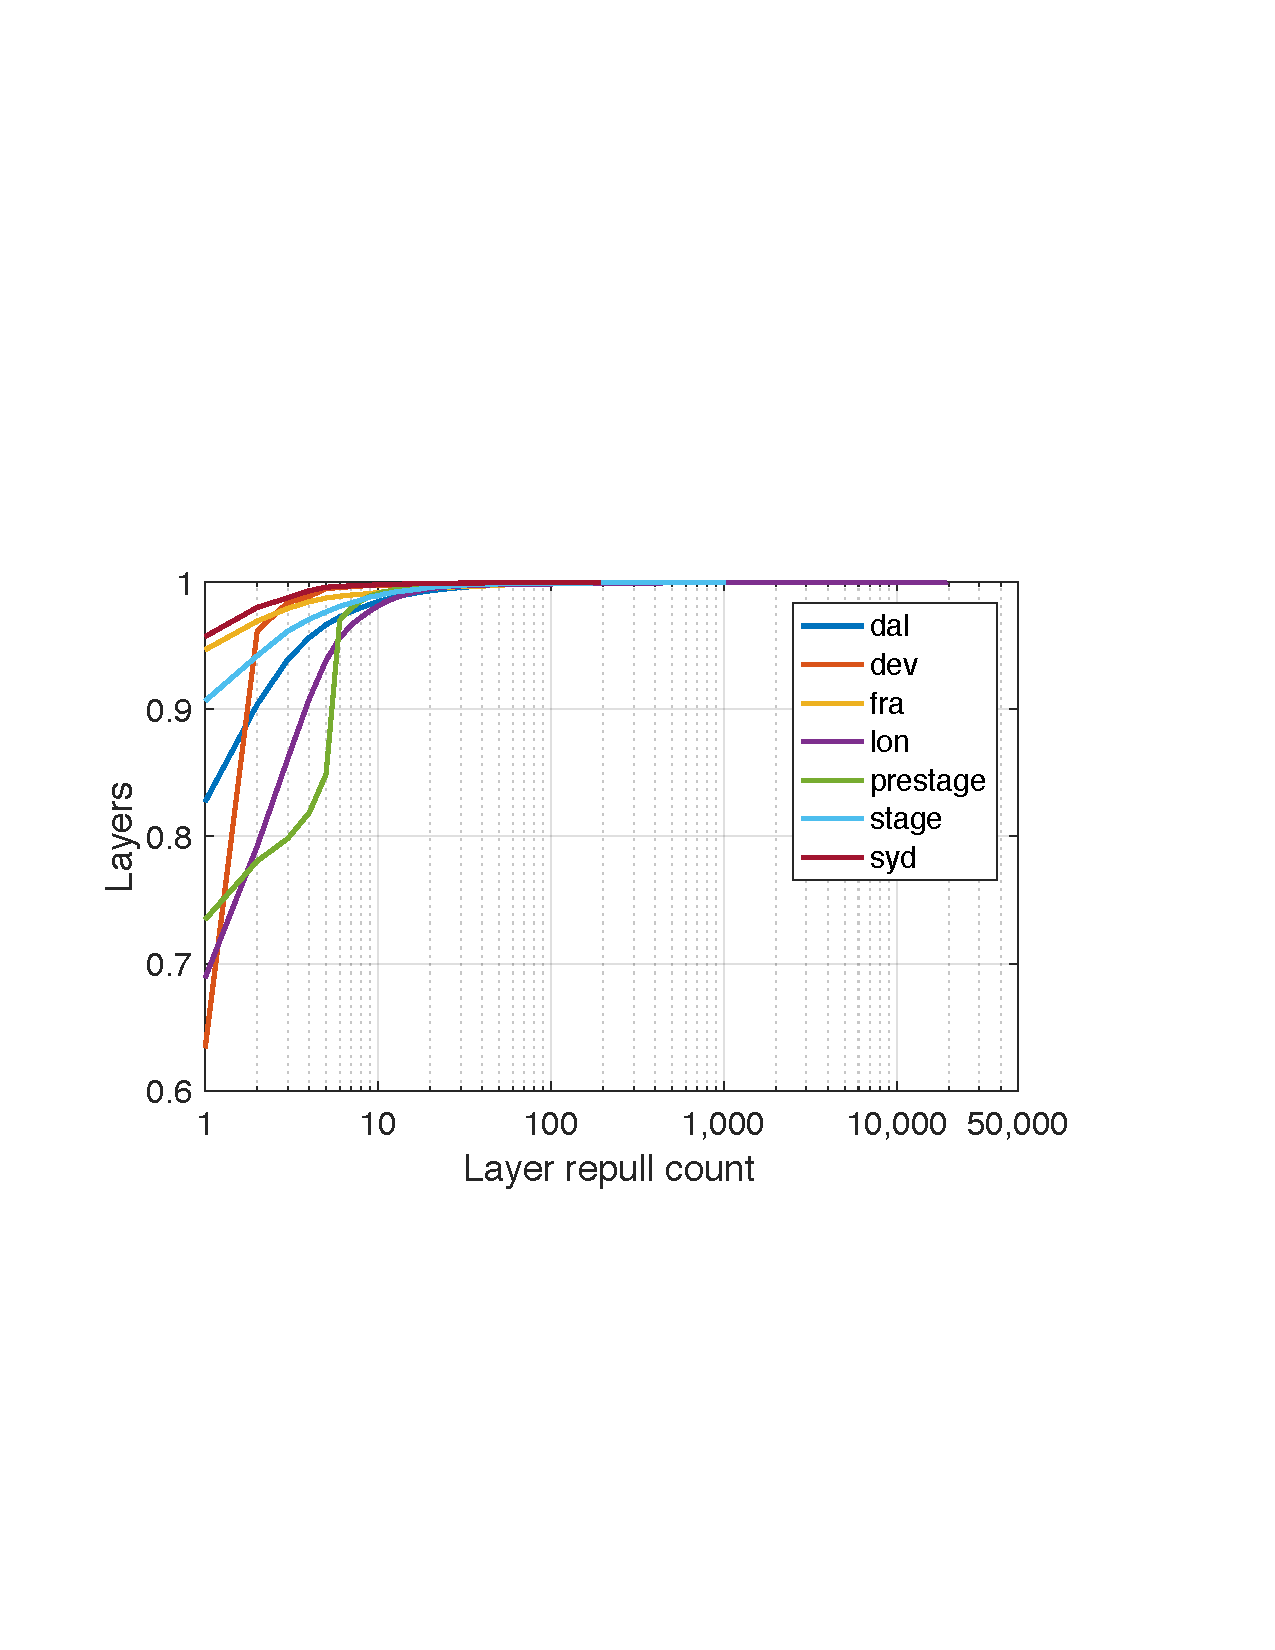
\includegraphics[width=1\textwidth]{graphs/cdf-layer-repull-by-same-client.pdf}
%			%\caption{CDF of layer repull count.}
%		%	\vspace{-3pt}
%			\label{fig:layer-repull-cdf}
%		\end{minipage}
%			\begin{minipage}{0.32\linewidth}
%				\centering
%				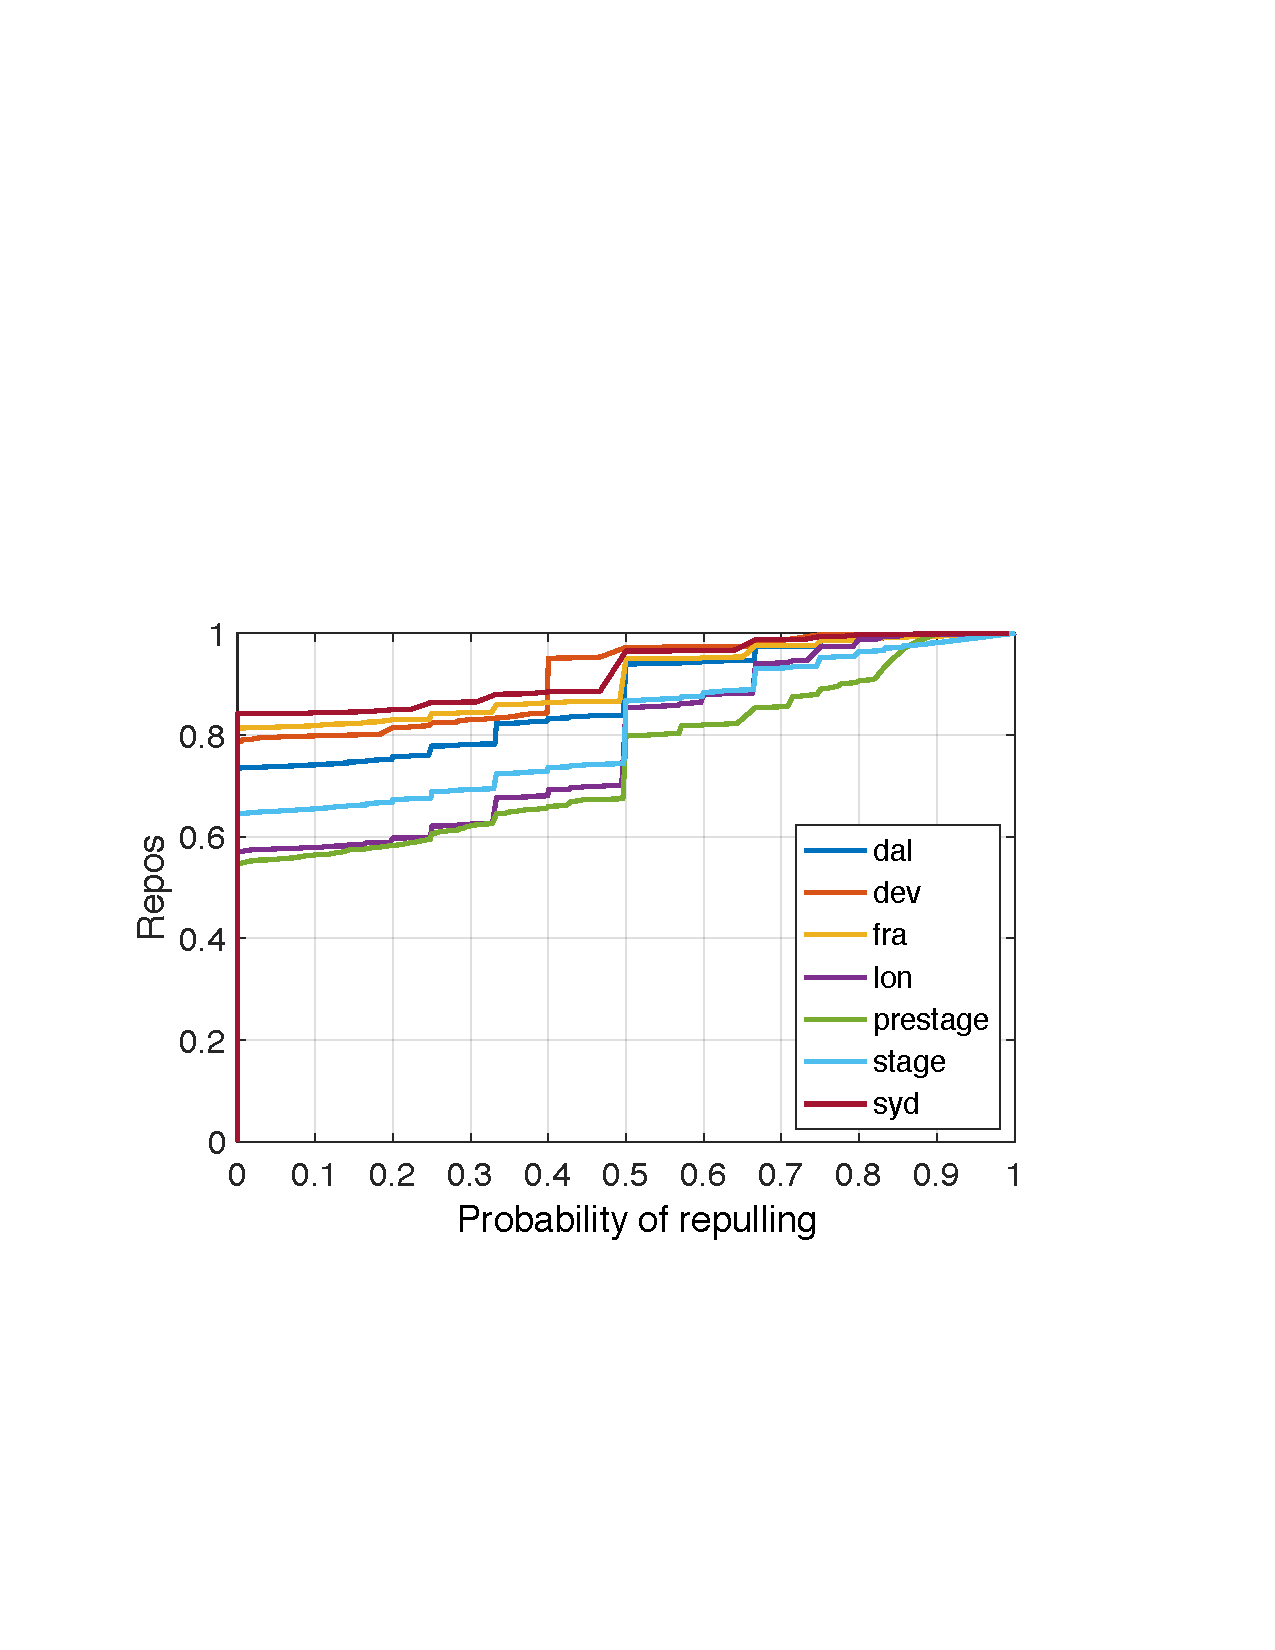
\includegraphics[width=1\textwidth]{graphs/cdf-repo-repull-ratio-by-same-client.pdf}
%				%\caption{PDF of repository repulling probability.}
%				%	\vspace{-3pt}
%				\label{fig:repo-repull-cdf}
%			\end{minipage}
%		\begin{minipage}{0.32\linewidth}
%			\centering
%			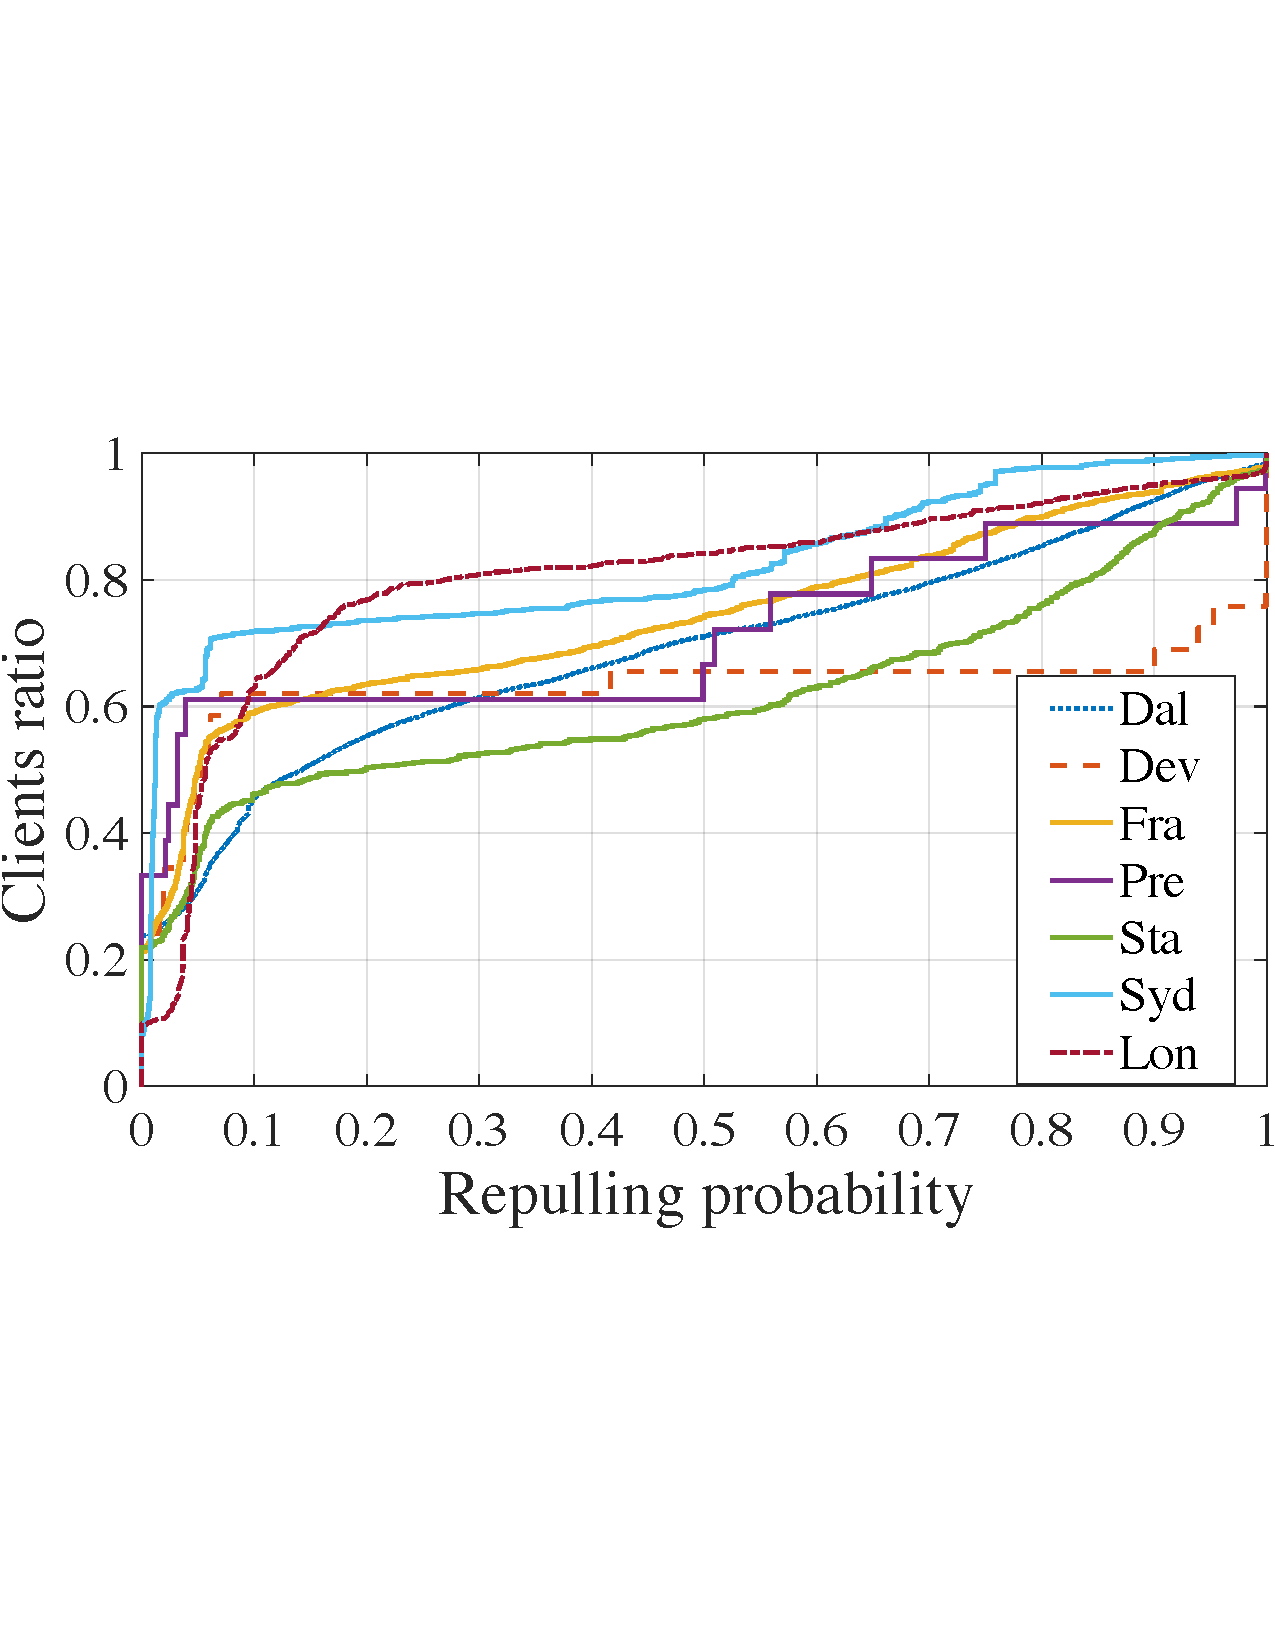
\includegraphics[width=1\textwidth]{graphs/cdf-client-repull-layer-request-ratio.pdf}
%			%
%			%	\vspace{-3pt}
%			\label{fig:client-repull-cdf}
%		\end{minipage}
%	\caption{PDF of client repull count, repository repulling probability, and client repulling probability..}
%\end{figure*}

%\begin{figure}[!t]
%	\centering
%	\subfigure[\texttt{GET} layer request count]{
%		\includegraphics[width=0.22\textwidth]{graphs/cdf-layer-repull-ratio-by-same-client.pdf}
%		\label{fig:layer-repull-cdf}
%	}
%%	\subfigure[Repository repulling probability]{
%%		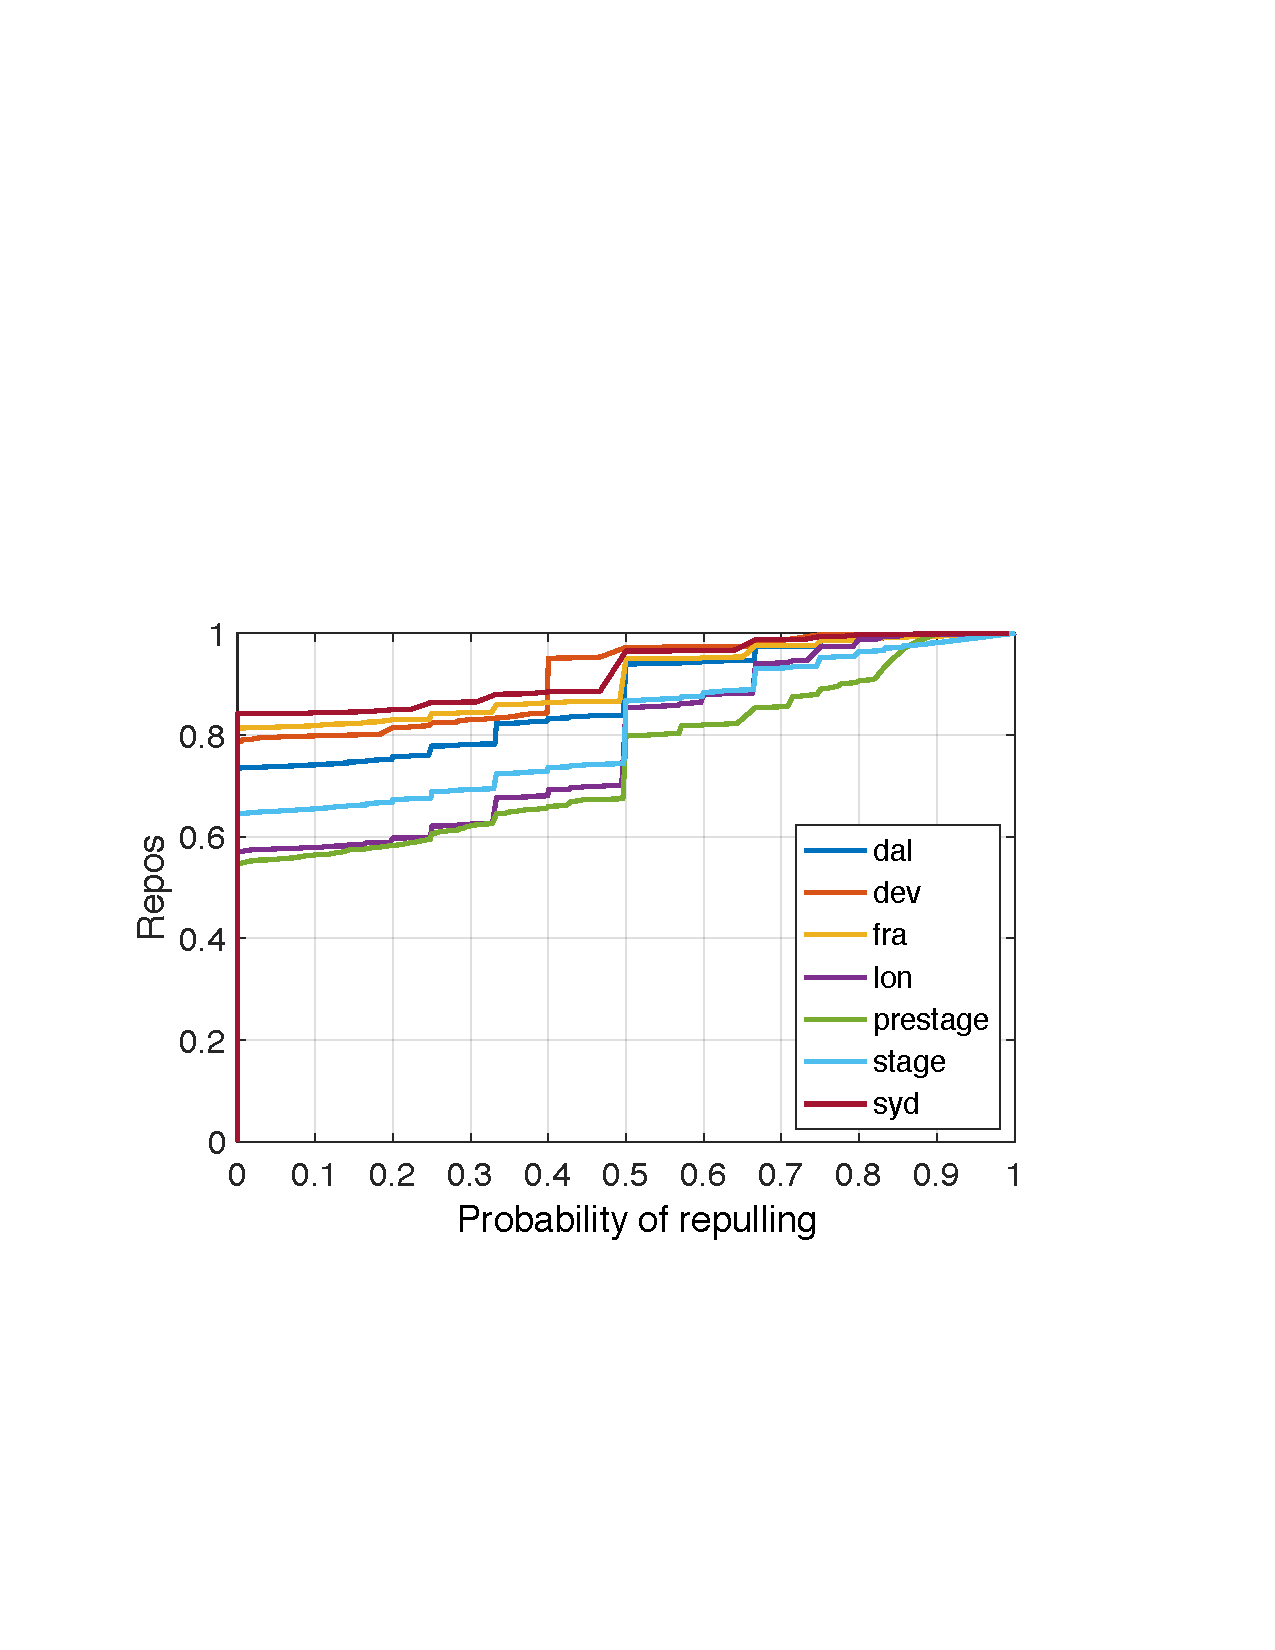
\includegraphics[width=0.2\linewidth]{graphs/cdf-repo-repull-ratio-by-same-client.pdf}
%%		\label{fig:repo-repull-cdf}
%%	}
%	\subfigure[Client repulling probability]{
%	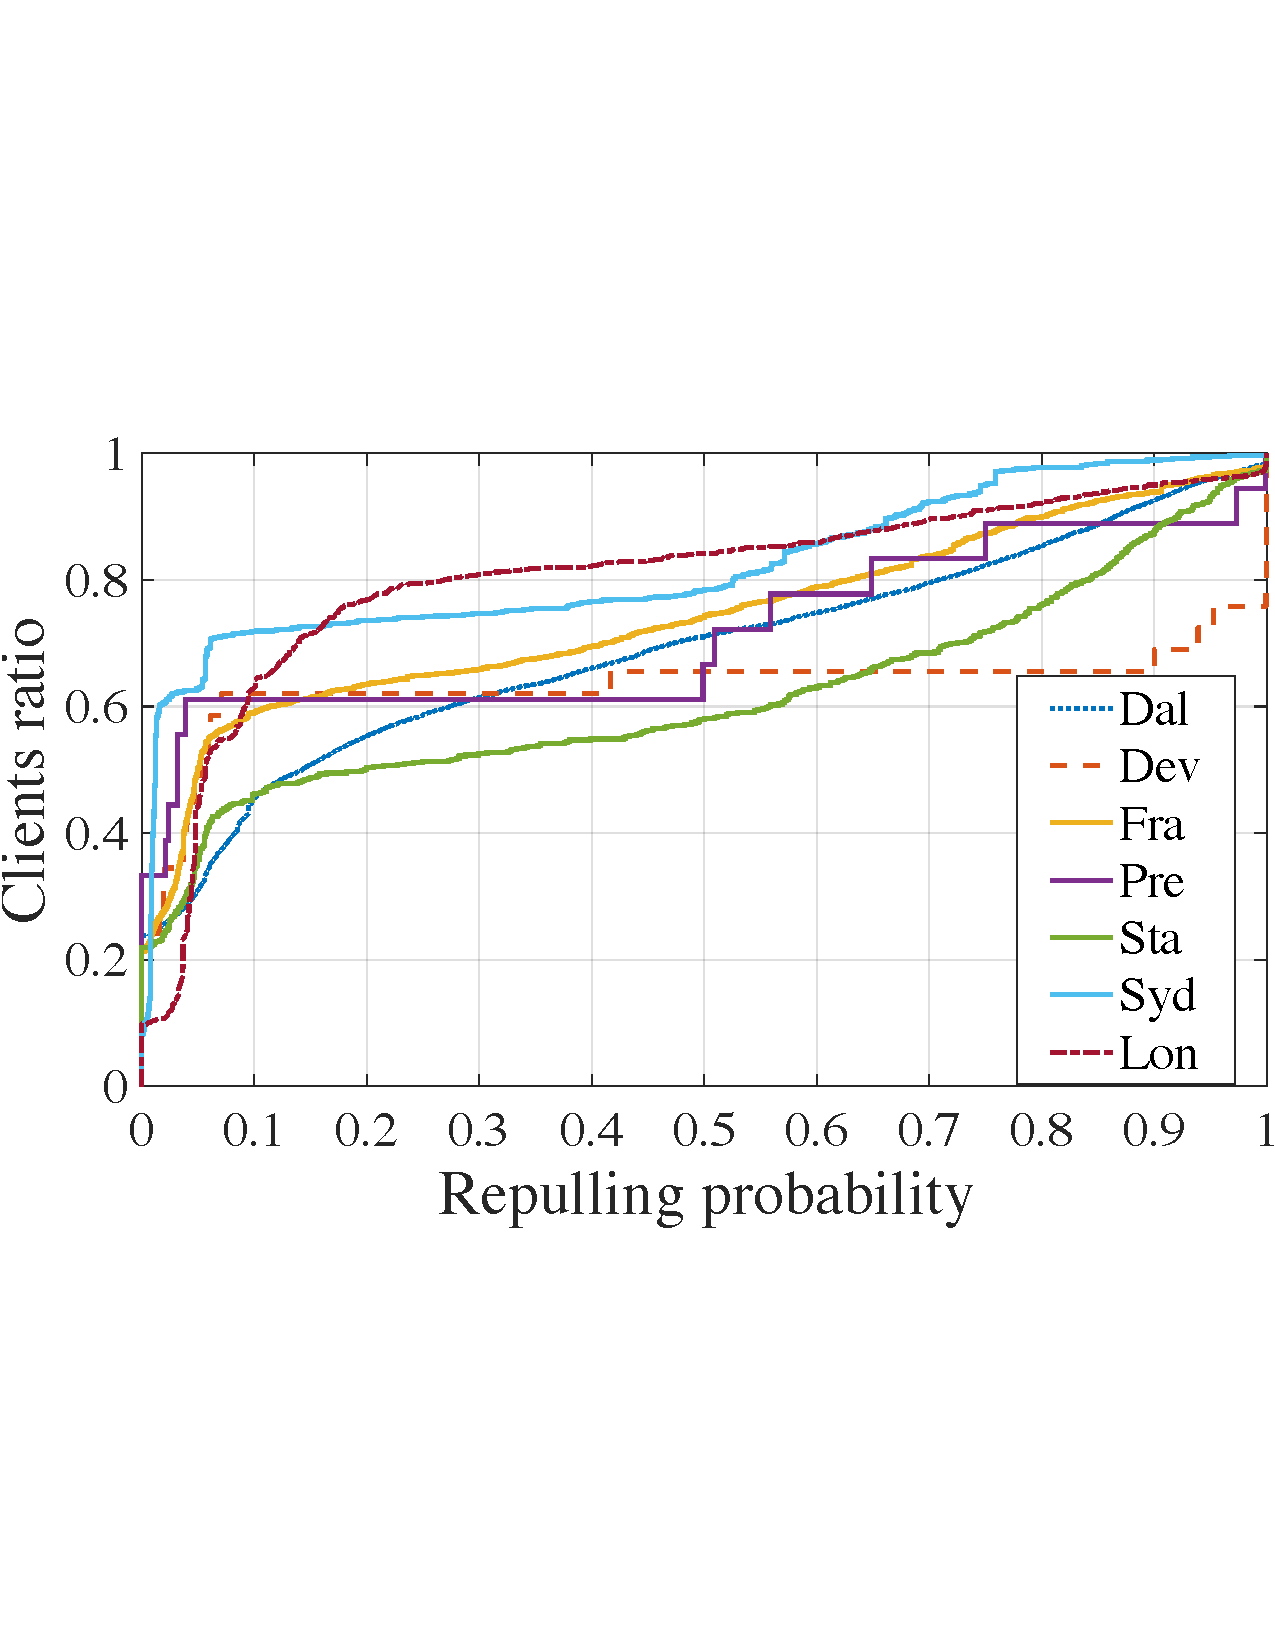
\includegraphics[width=0.2\textwidth]{graphs/cdf-client-repull-layer-request-ratio.pdf}
%   \label{fig:client-repull-cdf}
%}
%	\caption{CDF of \texttt{GET} layer request count and client repulling probability.}
%	\label{fig-repull}
%\end{figure}
%






\begin{figure*}[t]
        \centering
        \begin{minipage}{0.3\textwidth}
                \centering
                \includegraphics[width=0.9\textwidth]{{graphs/cdf-layer-repull-ratio-by-same-client.pdf}
                \caption{CDF of \texttt{GET} layer request count}
                \label{fig:layer-repull-cdf}
        \end{minipage}%
        \begin{minipage}{0.3\textwidth}
                \centering
                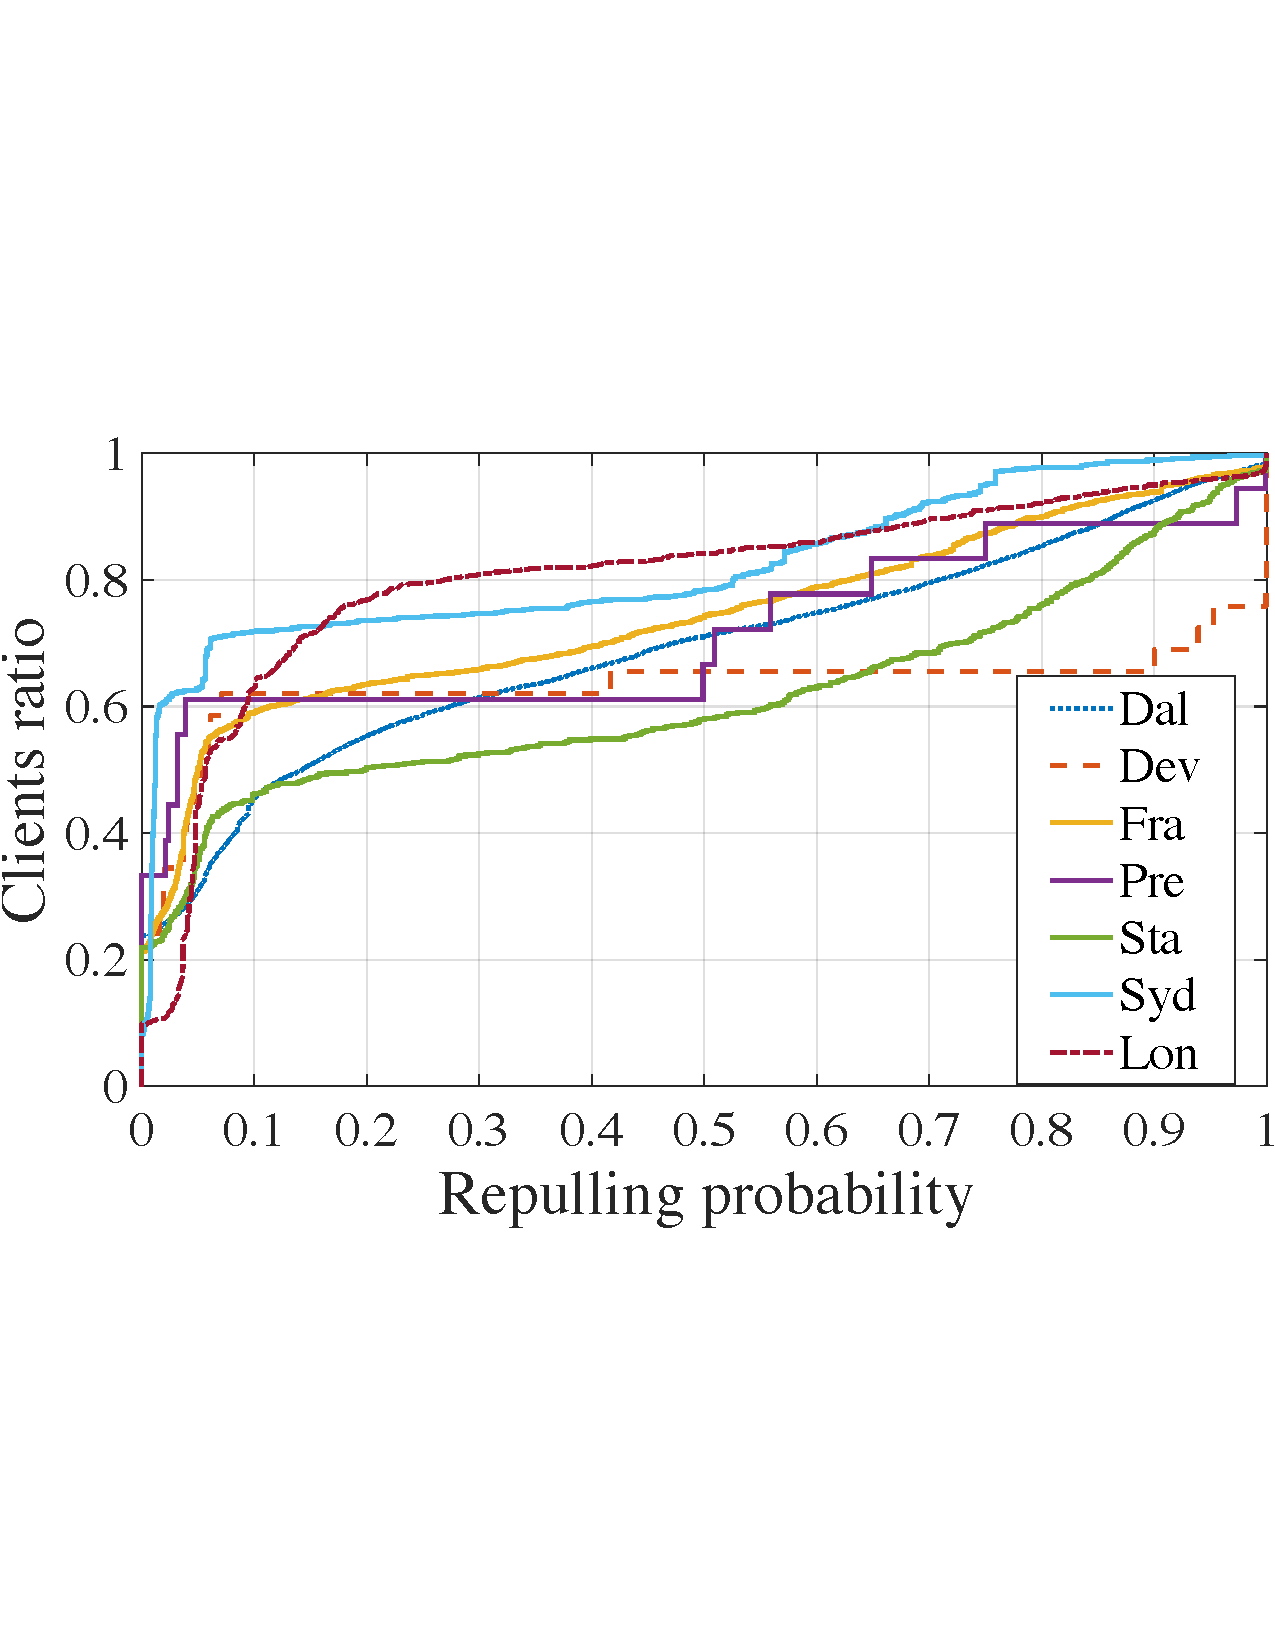
\includegraphics[width=0.9\textwidth]{graphs/cdf-client-repull-layer-request-ratio.pdf}
                \caption{CDF of Client repulling probability}% of LRU cache and preconstruct cache.}
                \label{fig:client-repull-cdf}
        \end{minipage}%
        \begin{minipage}{0.3\textwidth}
        \centering
        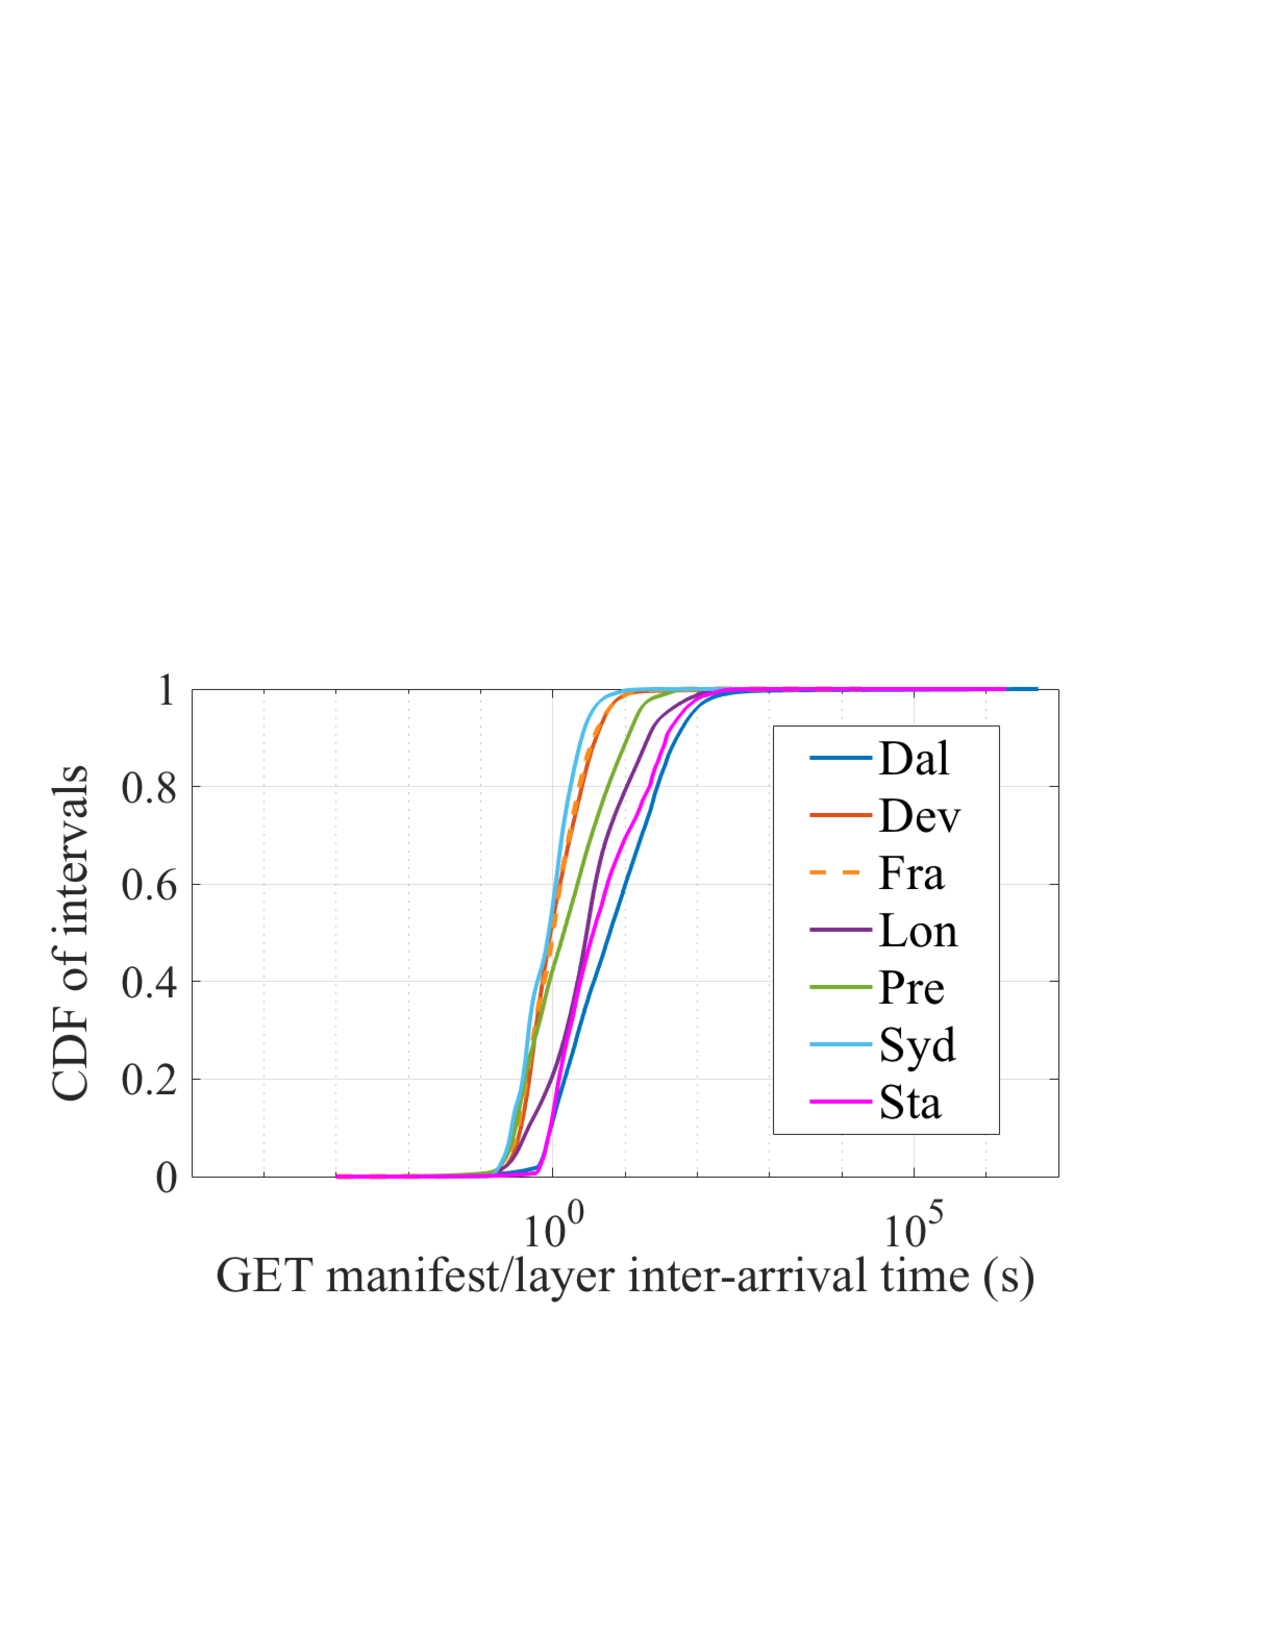
\includegraphics[width=0.9\textwidth]{graphs/GML-intervals.pdf}
        \caption{Intervals between \texttt{GET} manifest request and \texttt{GET} layer request}
        \label{fig:intervals}
   \end{minipage}
\end{figure*}





%\begin{figure}[!t]
%	\centering
%	\subfigure[CDF of compression ratio]{\label{fig_cdf_compression_ratio}
%		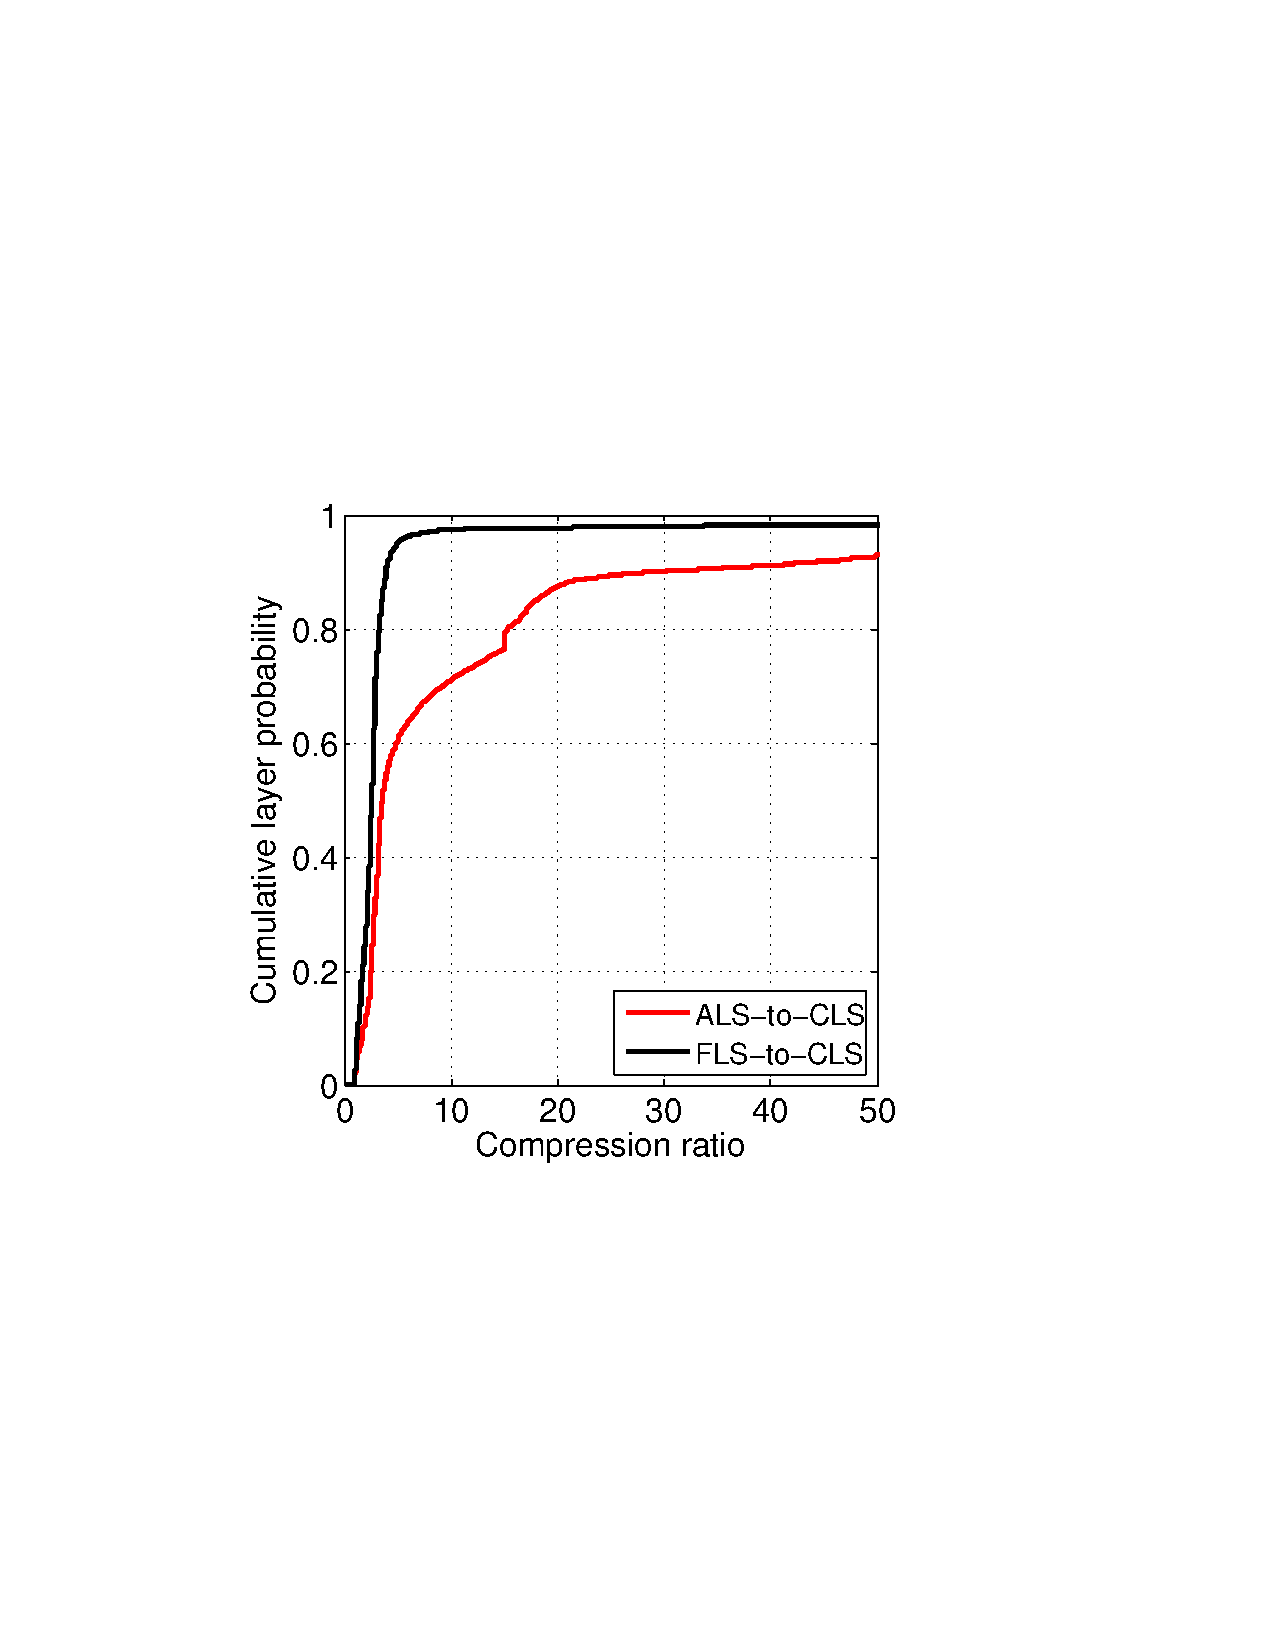
\includegraphics[width=0.23\textwidth]{graphs/cdf_compression_ratio.pdf}
%	}
%	\subfigure[Histogram of comp. ratios]{\label{fig_his_compression_ratio}
%		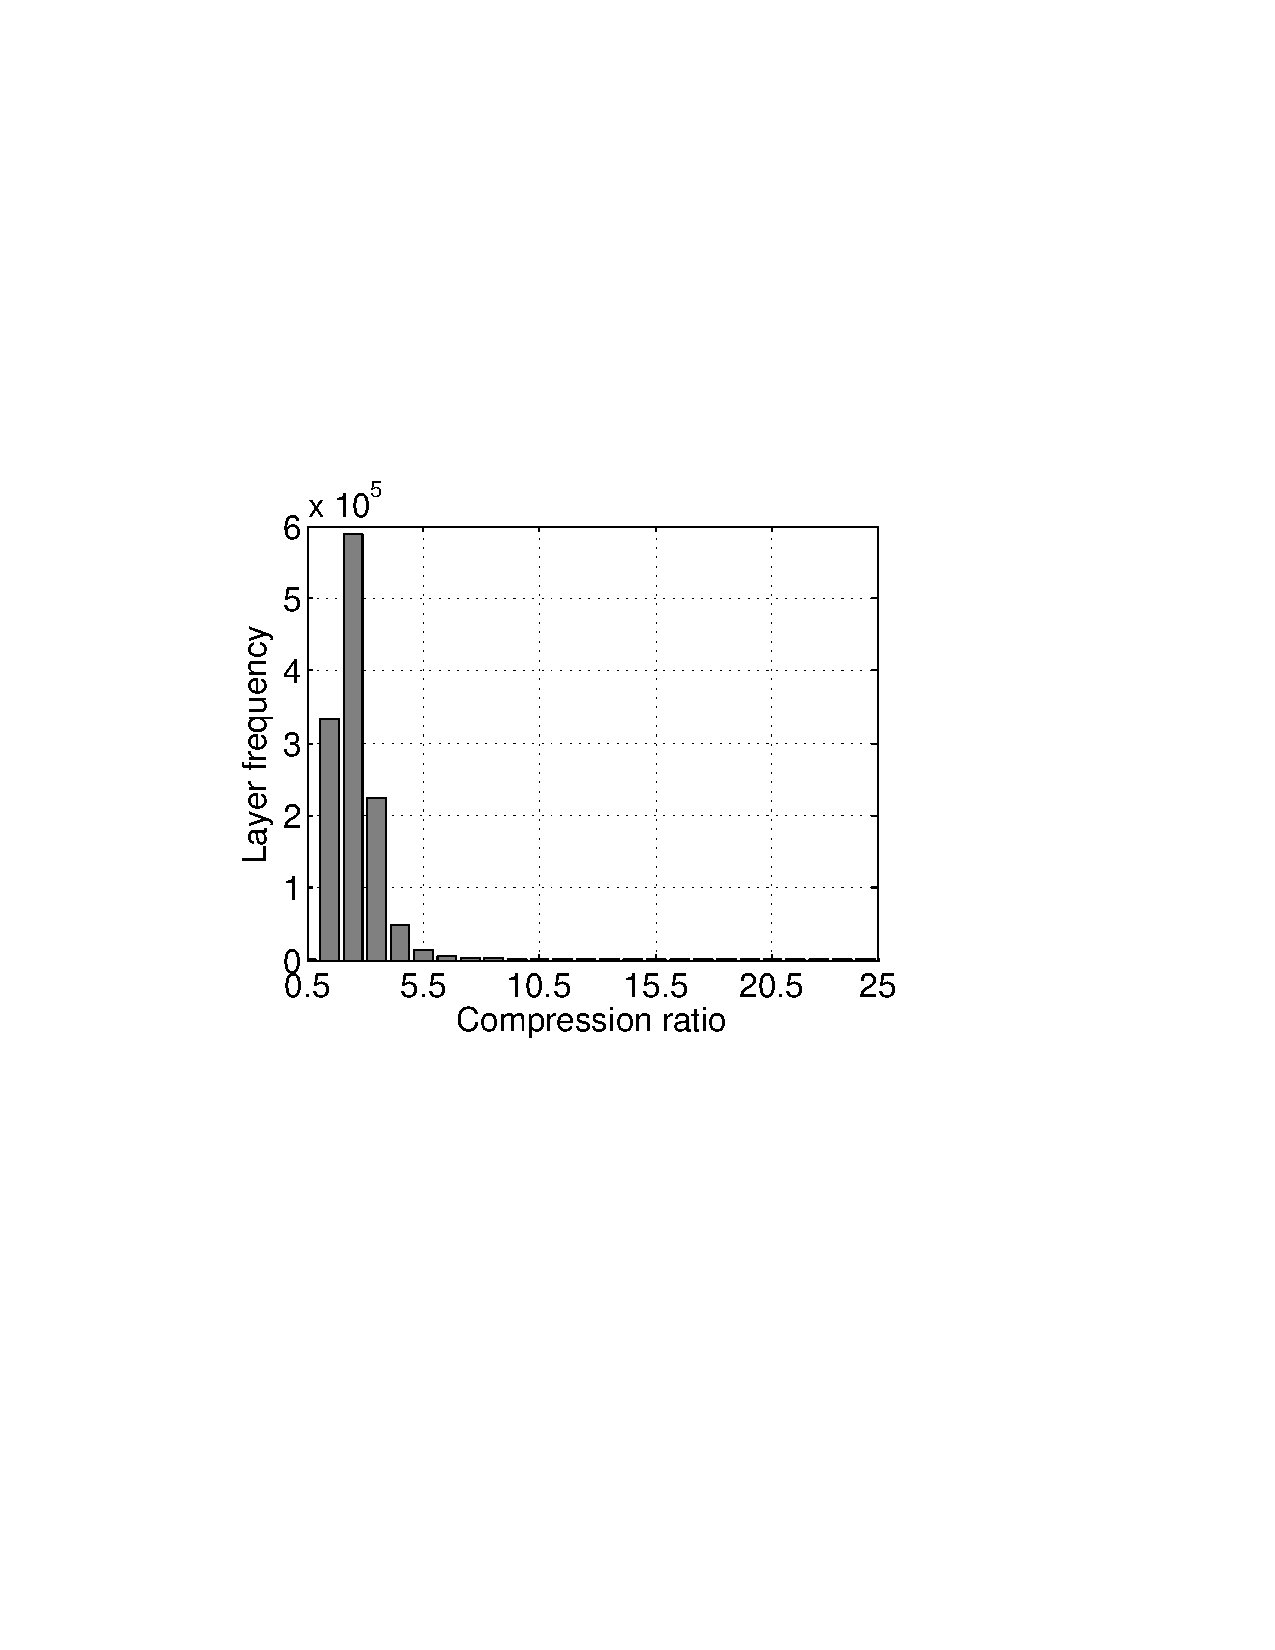
\includegraphics[width=0.223\textwidth]{graphs/his_compression_ratio.pdf}
%	}
%	\caption{Layer compression ratio distribution
%		%\vcomment{Different colors are used in figure (a) and (b) FLS/CLS\nancomment{will address later}}
%	}
%	\label{fig-compression-ratio}
%\end{figure}


%\begin{figure}[t]
%	\centering
%	\begin{minipage}{0.26\textwidth}
%		\centering
%		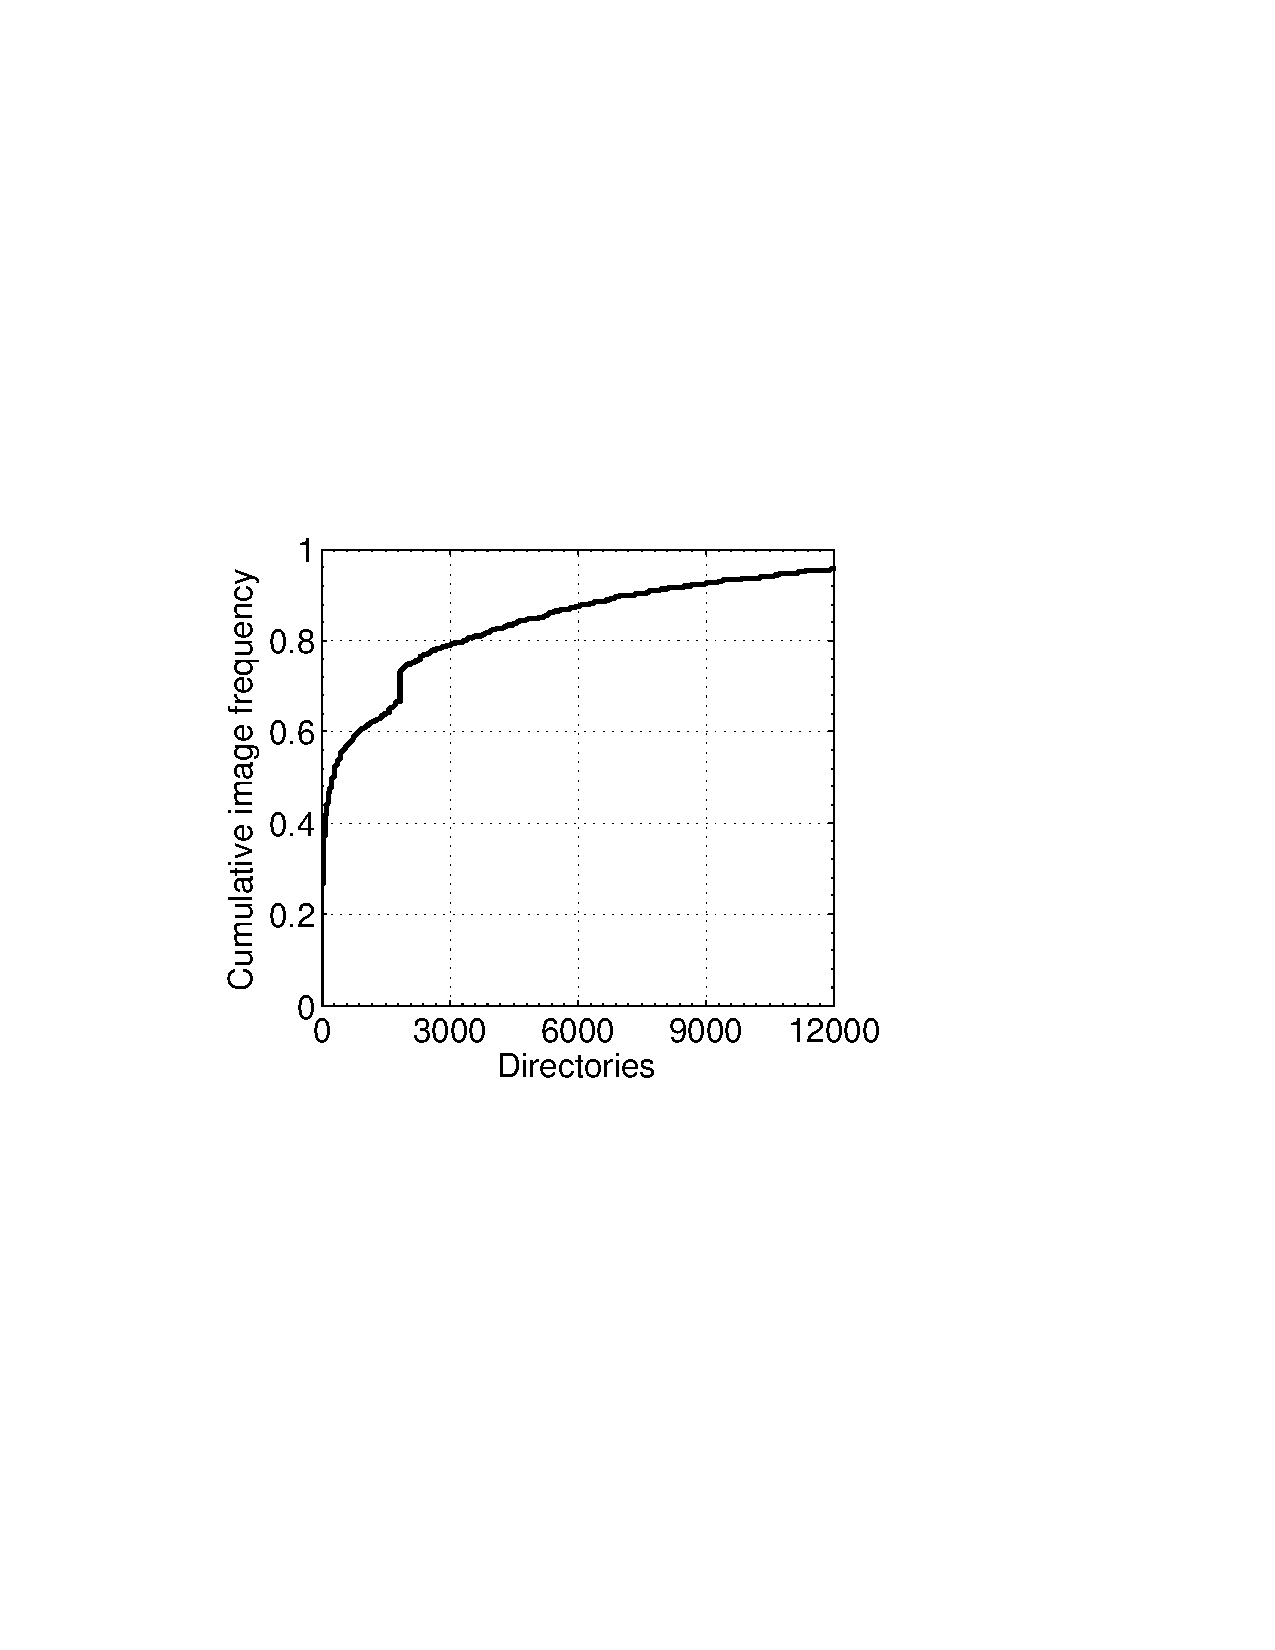
\includegraphics[width=1\textwidth]{graphs/dir.pdf}
%		\caption{CDF of images by\newline directories}
%		\label{fig-dir}
%	\end{minipage}%
%	\begin{minipage}{0.24\textwidth}
%		\centering
%		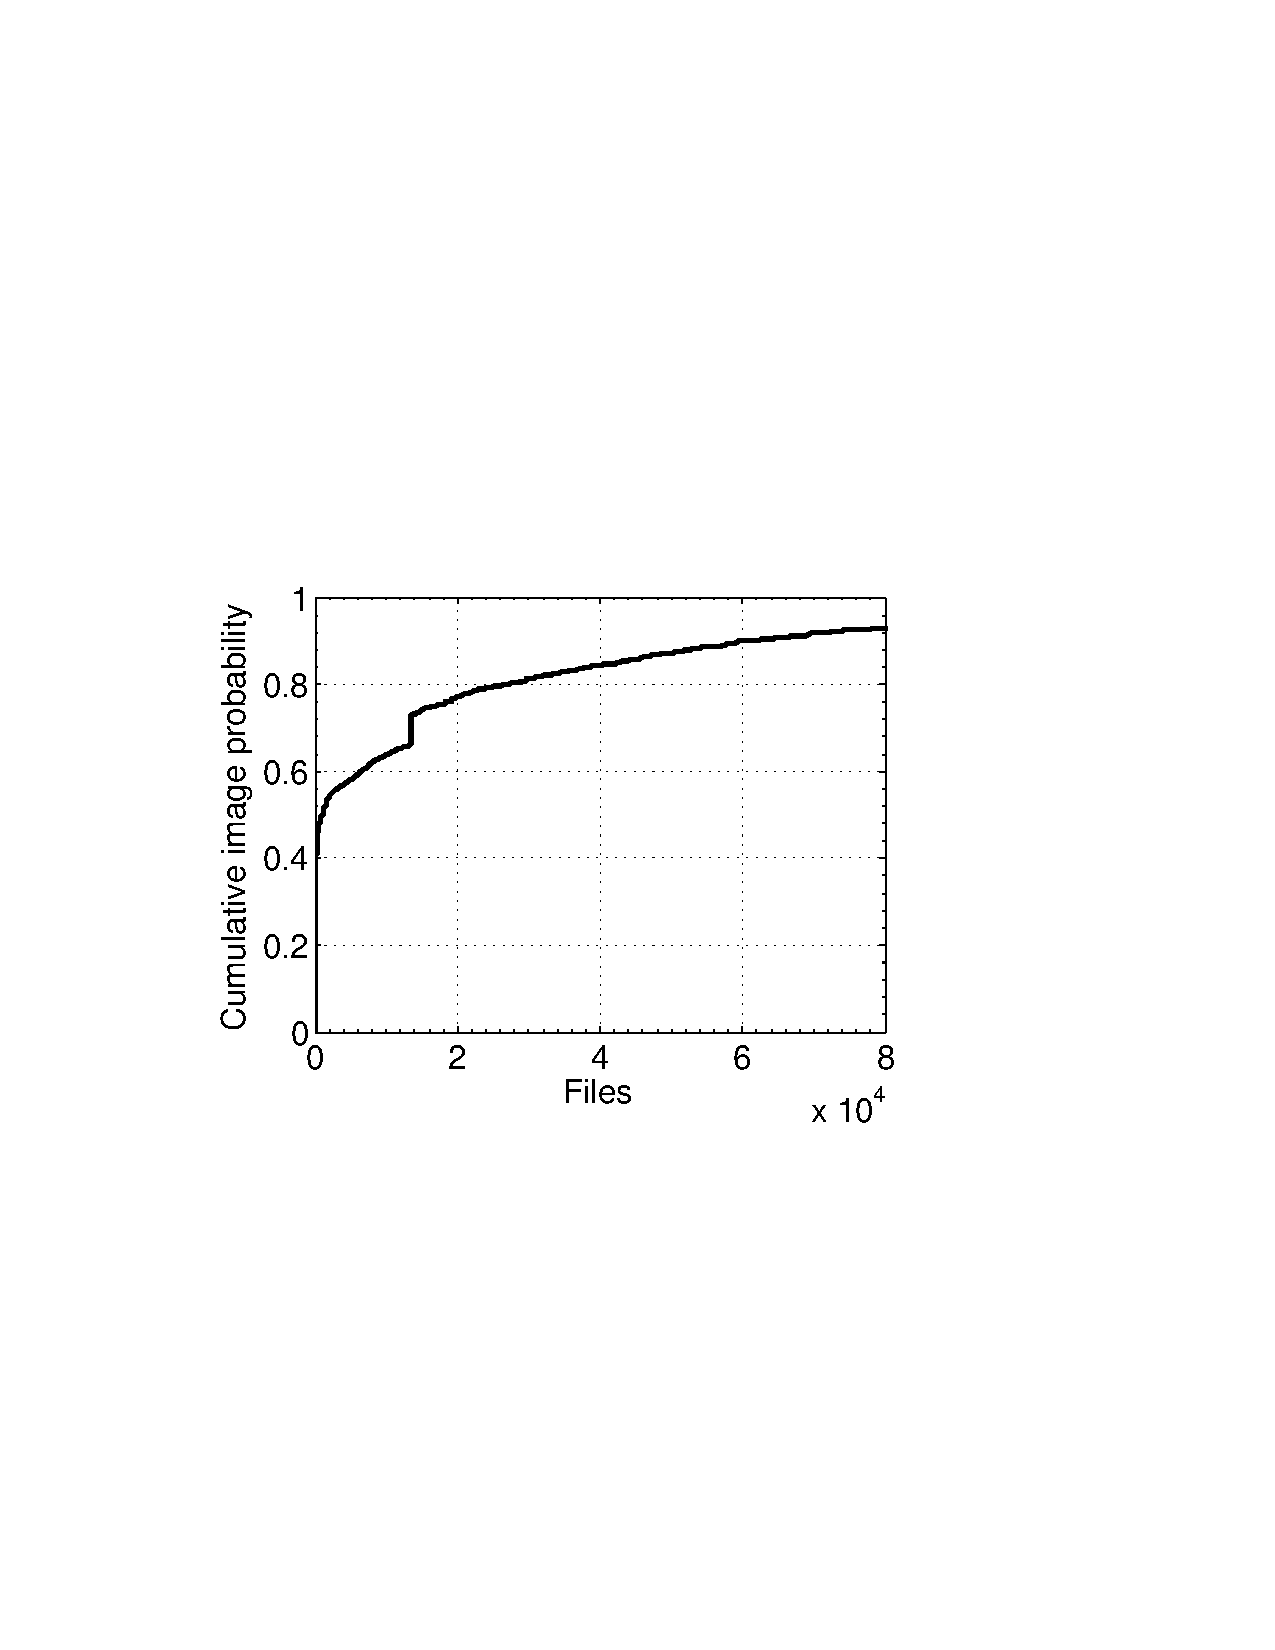
\includegraphics[width=1\textwidth]{graphs/file.pdf}
%		\caption{CDF of images by files}
%		\label{fig-file}
%	\end{minipage}
%\end{figure}

%\begin{figure}[htbp] 
%	\begin{minipage}{0.5\linewidth} 
%		\centering 
%		\includegraphics{circle} 
%		\caption{A Circle} 
%		\label{fig:circle} 
%	\end{minipage}% 
%	\begin{minipage}{0.5\linewidth} 
%		\centering 
%		\includegraphics{rectangle} 
%		\caption{A Rectangle} 
%		\label{fig:rectangle} 
%	\end{minipage} 
%\end{figure}


%<<<<<<< HEAD
\paragraph{User access patterns} 
When a Docker client \texttt{pulles} an image from Docker registry,
it will first \texttt{pull} the \textbf{manifest} of the image, 
which is metadata file of the image and contains a list of layers' digests.
After that, the client parses the manifest, gets a list of layers referenced by the image,
and compares against a \emph{local layer index}.
If a layer doesn't exist in the local layer index,
 the client will \texttt{pull} this layer.
 Thus, we can maintain a \emph{user local layer index} on registry side to keep track of user access history
 and predict which layer will be \texttt{pulled} by the user when the user issues a \texttt{pulling} manifest request.

Typically, if a layer is already stored locally,
then the client will not \texttt{pull} this layer again.
However, for Kubernetes,
users can configure different \emph{pull policies}, 
such as \emph{IfNotPresent (i.e, pulling if not present)} or \emph{Always pulling}.
We observe these two kinds of user behaviors in the real world workloads~\cite{xxx} as follows:
%we observe that few clients pull the same layers multiple time

\paragraph{Pull once VS. Always pull}
Figure~\ref{fig:layer-repull-cdf} shows the CDF of layer \texttt{pull} count by the same clients. 
%Here, \emph{repulling} indicates the act of pulling layers that have been pulled by the user before because they are no longer present on the user side.
Majority of layers are only pulled once by the same clients.
%83\% of the layers are only pulled twice.
For example, only 97\% of layers from \texttt{Syd} are only pulled once by the same clients.
We also observe that few clients \emph{pull} the same layers continuously.
For example, a client from \texttt{Lon} pulls the same layer 19,300 times.
%When different clients \texttt{pull} the same repository, 
%they will fetch different amount of layers from the repository based on the contents of their local layer dataset. 
%The local layers can vary with time due to clearing of the data so the same clients can fetch different amounts of layers at different times.
%Therefore, a \texttt{pull manifest} request doesn't usually result in repulling all the layers in the repository. 
%Here, we define \emph{repulling a repository} as repulling the layers in the repository for the same client.
%Figure~\ref{fig:repo-repull-cdf} shows the CDF of the probability of repository repulling, calculated 
%as the number of \texttt{pull manifest} resulting in repository repulling divided by 
%the total number of \texttt{pull manifest} requests issued for the same repository.
%We see that majority of repositories aren't repulled.
%The percentage of repositories whose repull probability is zero (i.e. are pulled only once by a client) ranges from 57\% for \texttt{Prestage} to 85\% for \texttt{Syd}.
%Only 20\% of repositories from  \texttt{Prestage}, \texttt{Stage}, and 
%\texttt{Syd} have a repulling probability higher than 0.5.
%We also observe that few repositories' repulling probability is 1, indicating repulls everytime by the clients.

We define \emph{repulling} as the act of pulling the same layer more than once by the same user.
% before because they are no longer present on the user side.
Figure~\ref{fig:client-repull-cdf} shows the client repulling probability, calculated as the number of \emph{repulling} layer requests divided by
the number of total \texttt{pull} layer requests issued by the same client.
We see that a significant amount of clients have a low repulling proability.
For example,
71\% of clients from \texttt{syd} have a repulling probability lower than 0.1.
Very few clients have a high repulling probability.
For instance,
only 2\% clients have a repulling probability higher than 0.9 from 
\texttt{Dal}.

We also observe that the slope is steep at both lower and higher probabilities.
But the slope becomes gentle in the middle.
For example, 
the slope at probabilities between 0.1 and 0.9 for \texttt{dev} almost equals to zero.
In this case,
the high repulling probability clients can be classified as always-pull clients, 
and the low repulling probability clients as pull-once clients. 
The few clients in the middle are considered as \emph{erratic}.
%
Thus,
to determine whether a client will \texttt{repull} a layer or not,
we consider the client repulling probability and the layer repull count.
%From the probability distribution of the clients repulling, we can observe that a significant chunk of the clients have very low repulling probability and another chunk of the clients have a very high repulling probability, with few clients in the middle. For simplicity of implementation, the high probability clients can be classified as always repulling clients, and the low probability clients as never repulling (i.e. they pull only once). The few clients in the middle are considered as \emph{erratic} and no classification is made for them.



\subsection{Layer preconstruction}
%%%\begin{figure*}[t]
%		\begin{minipage}{0.32\linewidth}
%			\centering
%			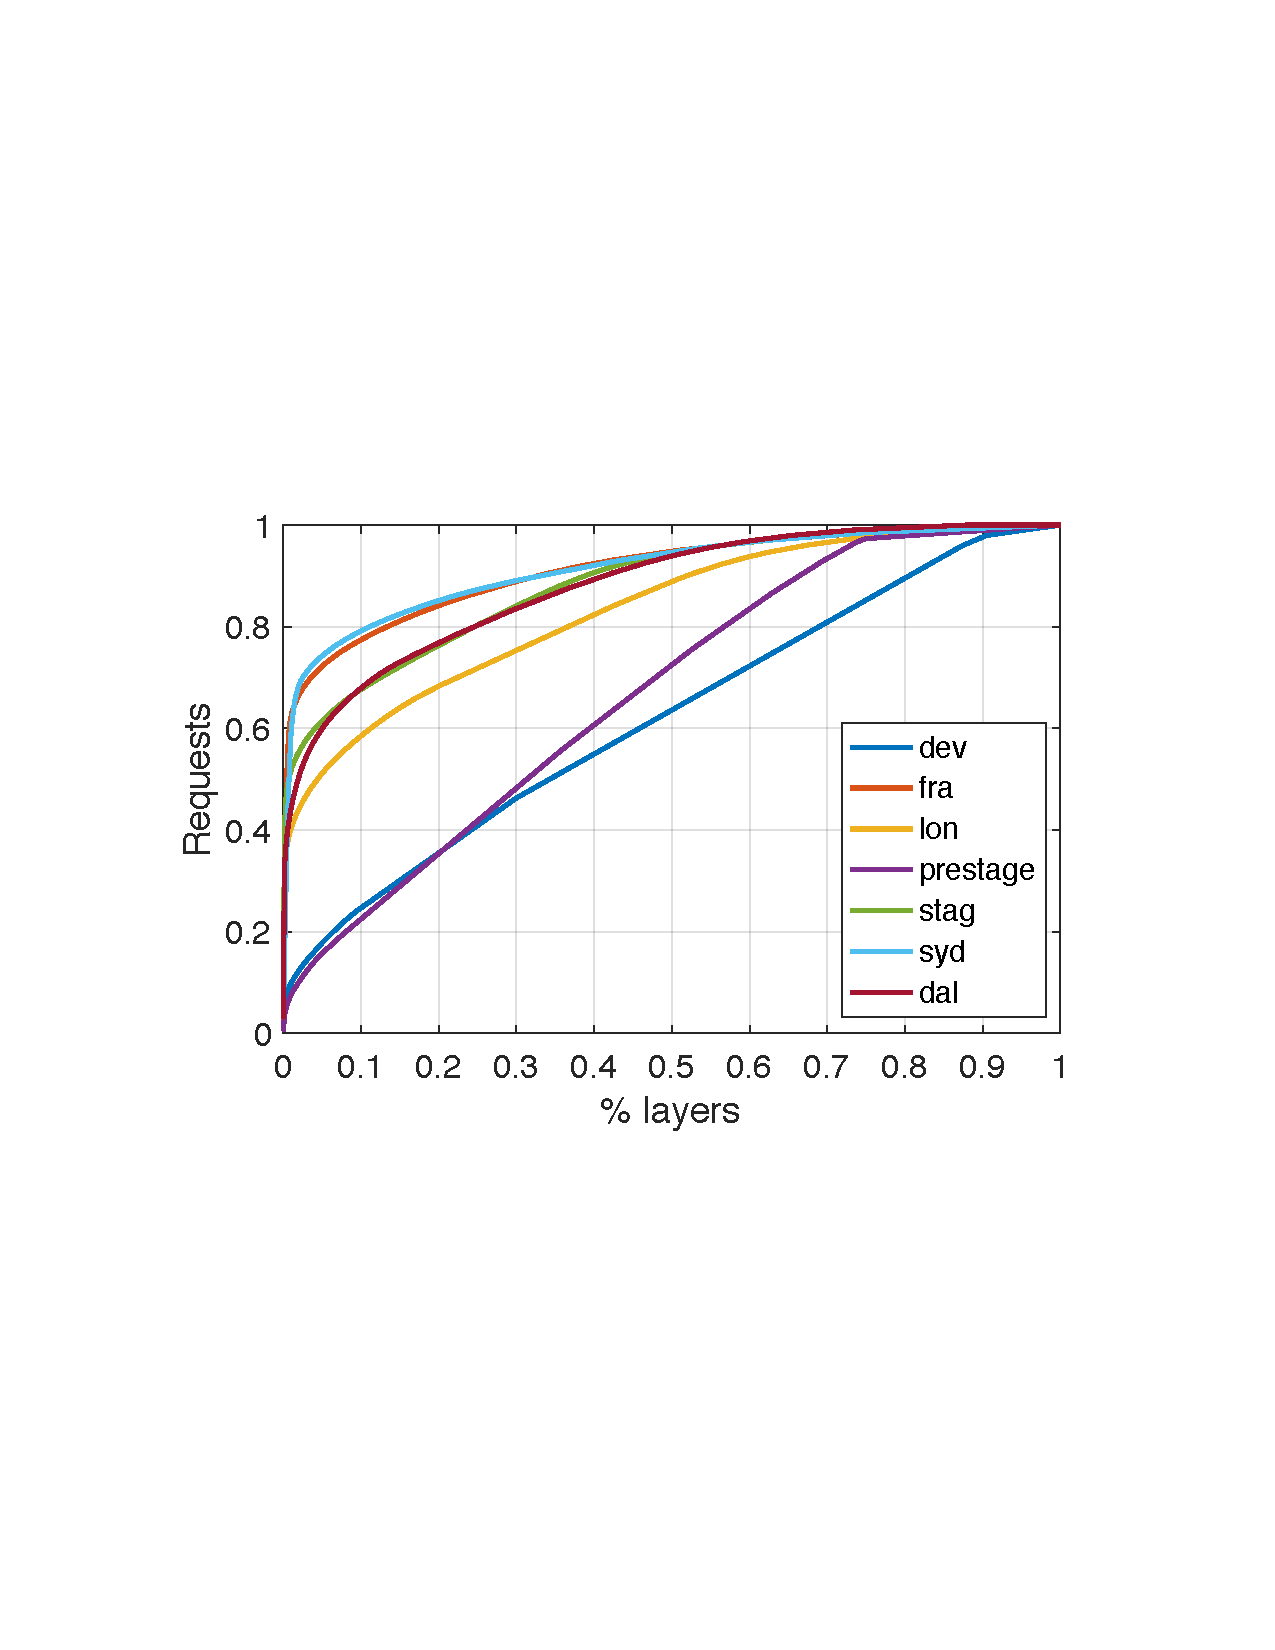
\includegraphics[width=1\textwidth]{graphs/layer_skewness.pdf}
%			%\caption{CDF of layer  count.}
%		%	\vspace{-3pt}
%			\label{fig:layer-skenwess}
%		\end{minipage}
%			\begin{minipage}{0.32\linewidth}
%				\centering
%				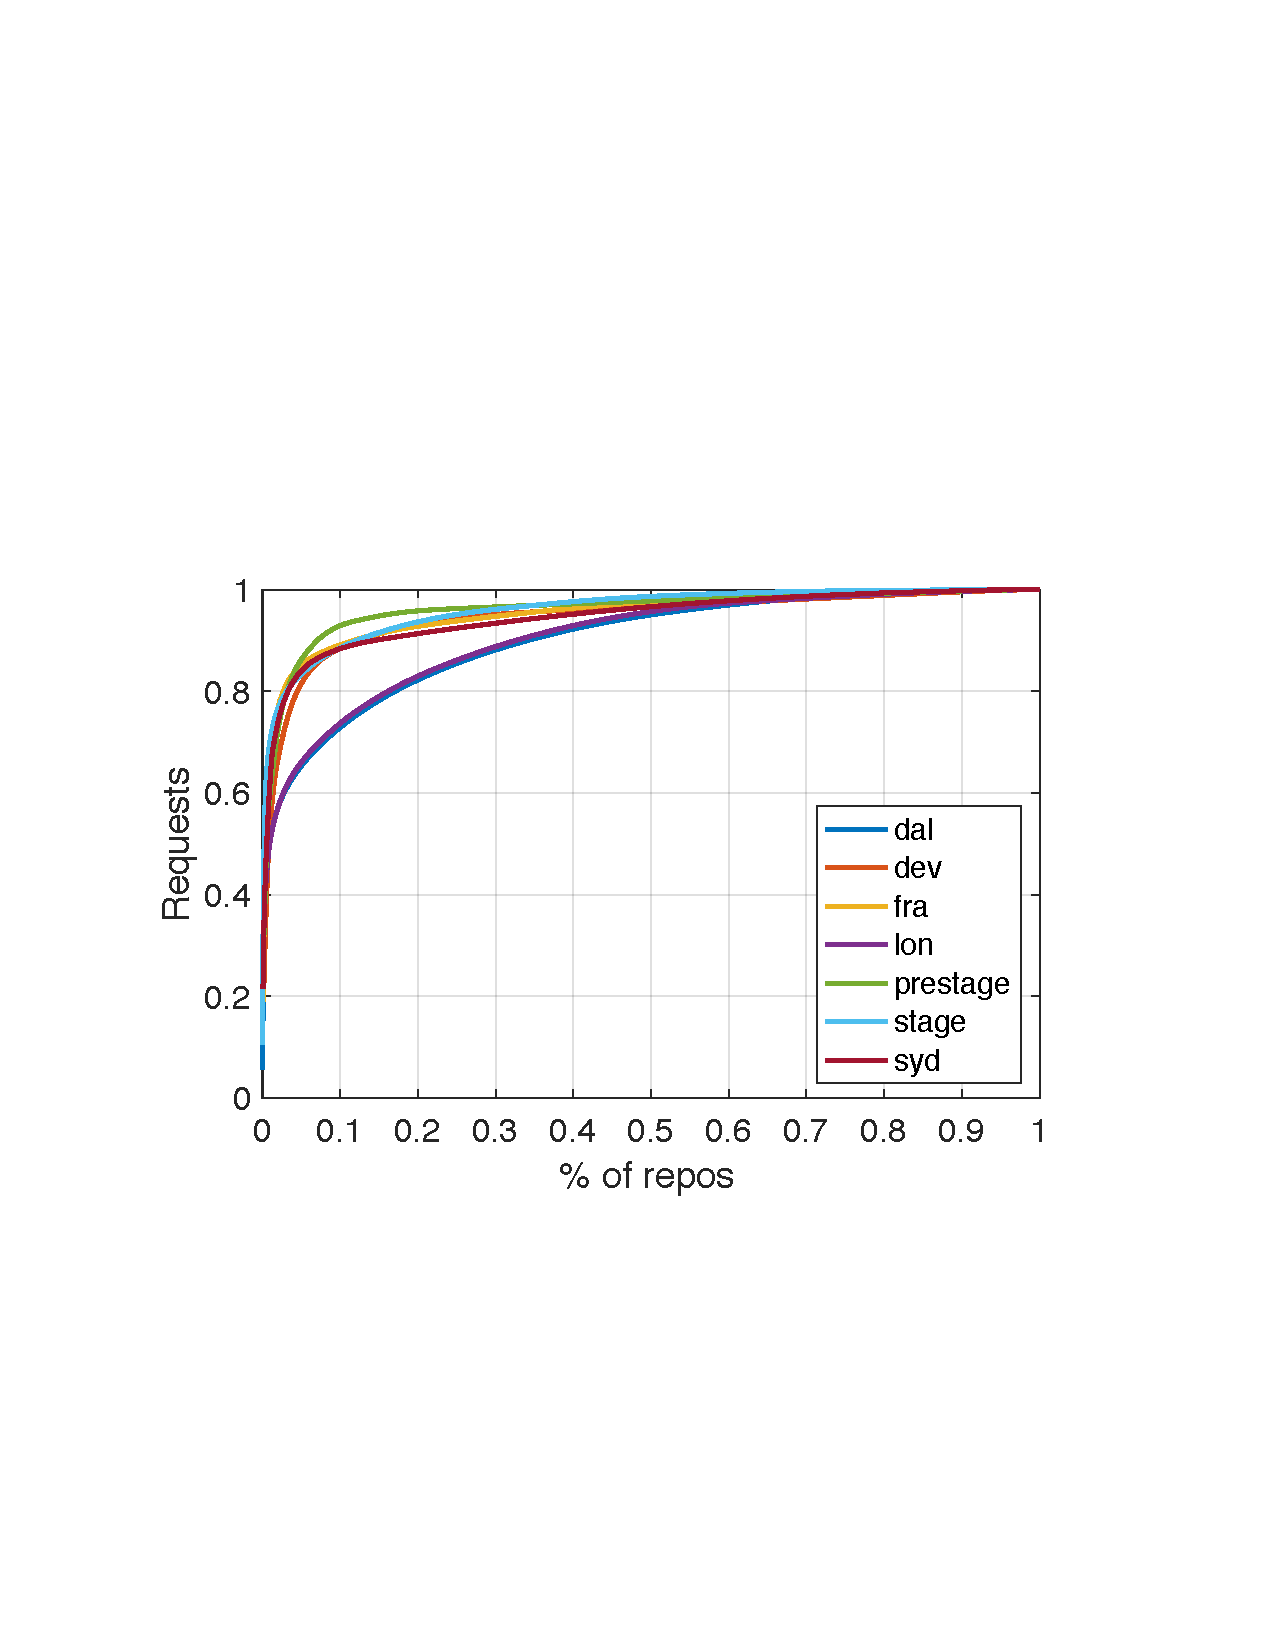
\includegraphics[width=1\textwidth]{graphs/repo-skewness.pdf}
%				%\caption{PDF of repository repulling probability.}
%				%	\vspace{-3pt}
%				\label{fig:repo-skewness}
%			\end{minipage}
%		\hfill
%		\begin{minipage}{0.32\linewidth}
%			\centering
%			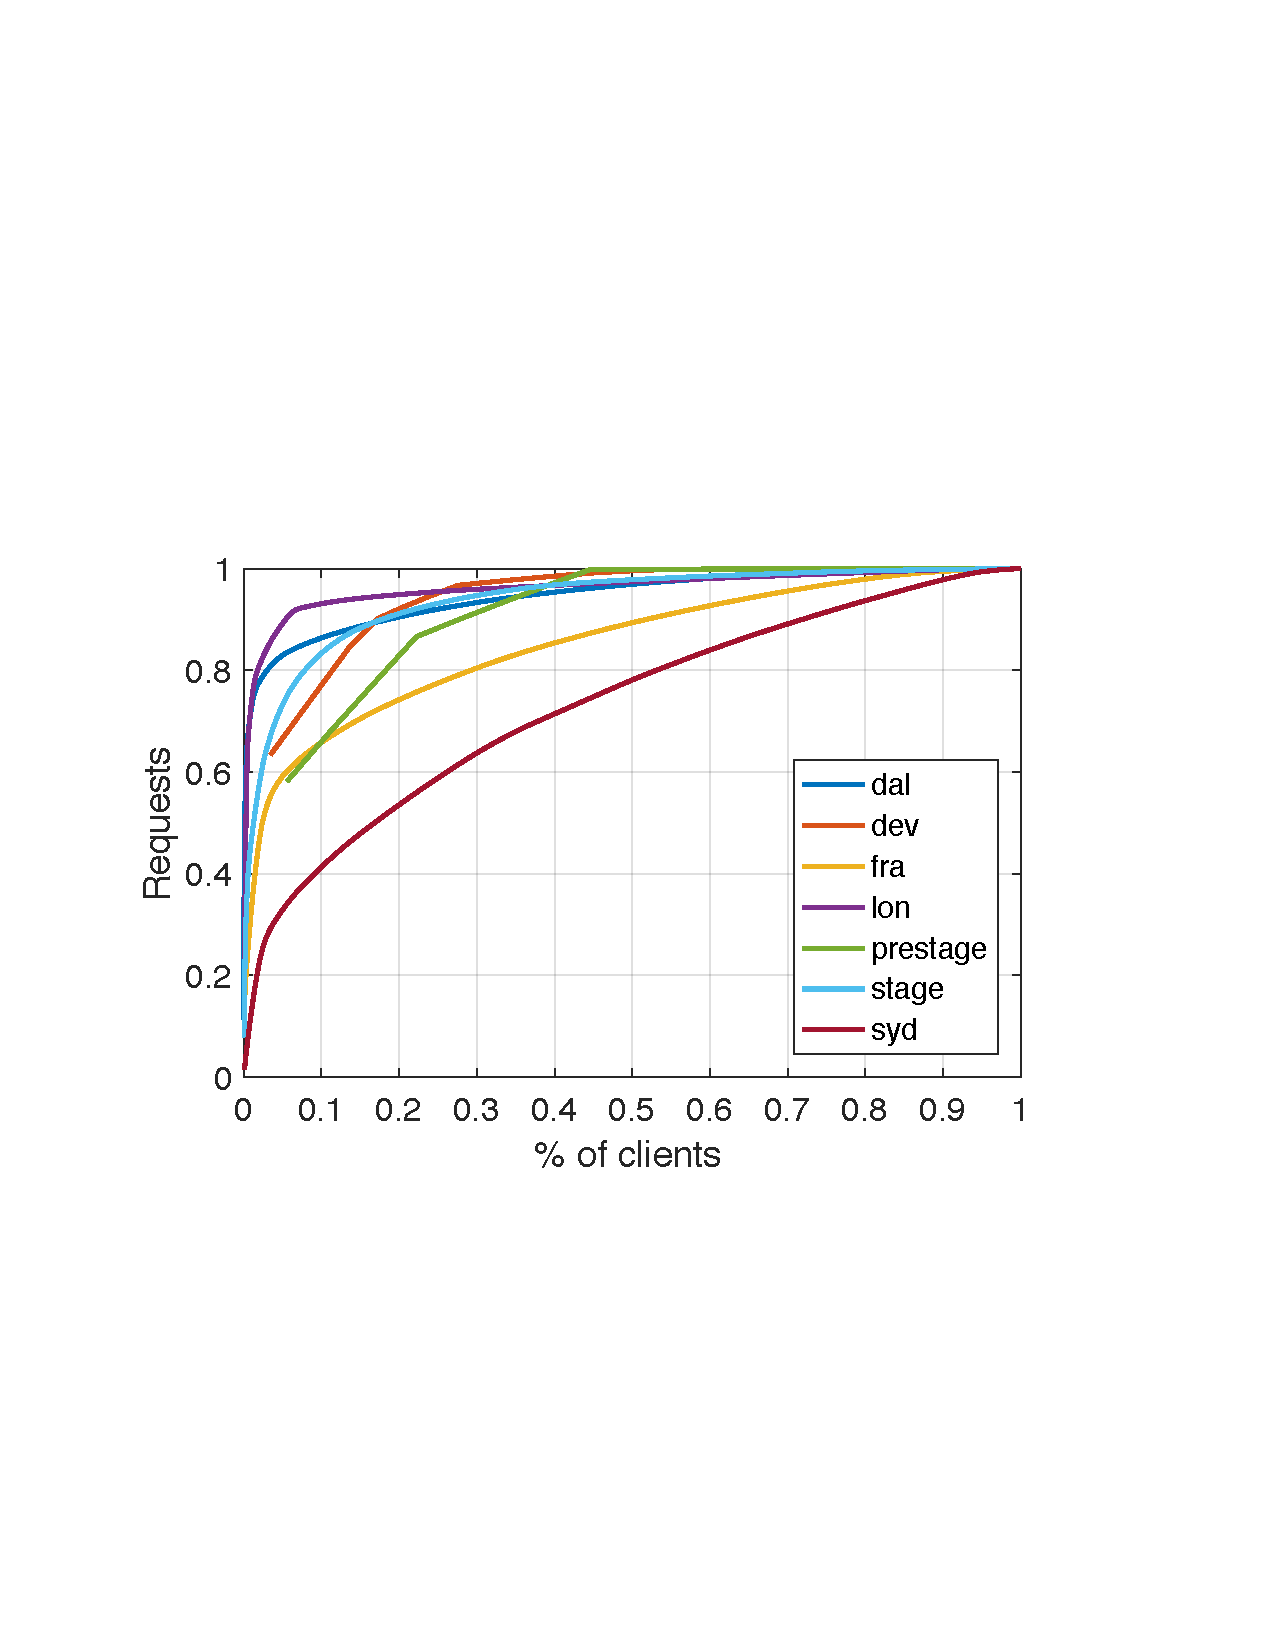
\includegraphics[width=1\textwidth]{graphs/client-skewness.pdf}
%			%\caption{PDF of client repulling probability.}
%			%	\vspace{-3pt}
%			\label{fig:client-skewness}
%			
%		\end{minipage}
%\caption{PDF of probability for layers, repositories, and clients.}
%%	\label{}
%\end{figure*}

\begin{figure*}[!t]
	\centering
	\subfigure[Layer repull count]{
		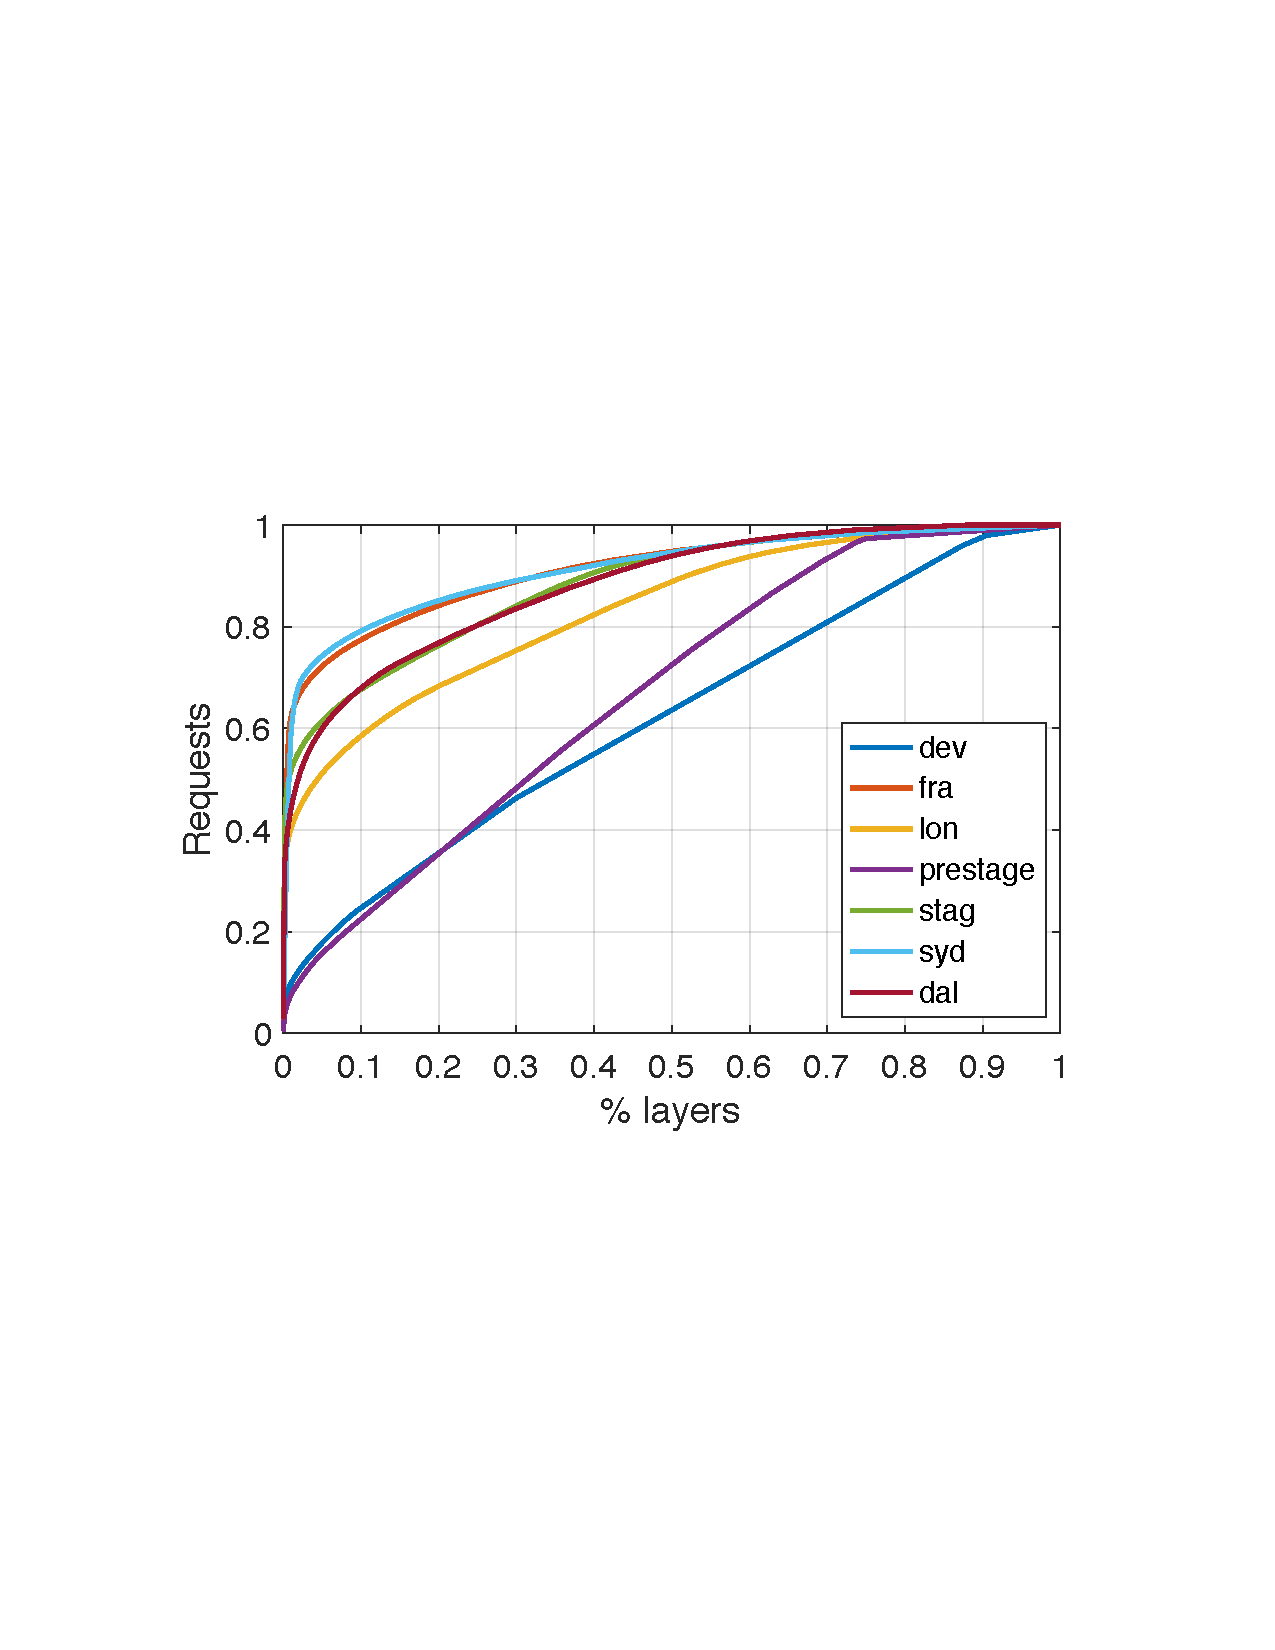
\includegraphics[width=0.2\linewidth]{graphs/layer_skewness.pdf}
		\label{fig:layer-skenwess}
	}
	\subfigure[Repository repulling probability]{
		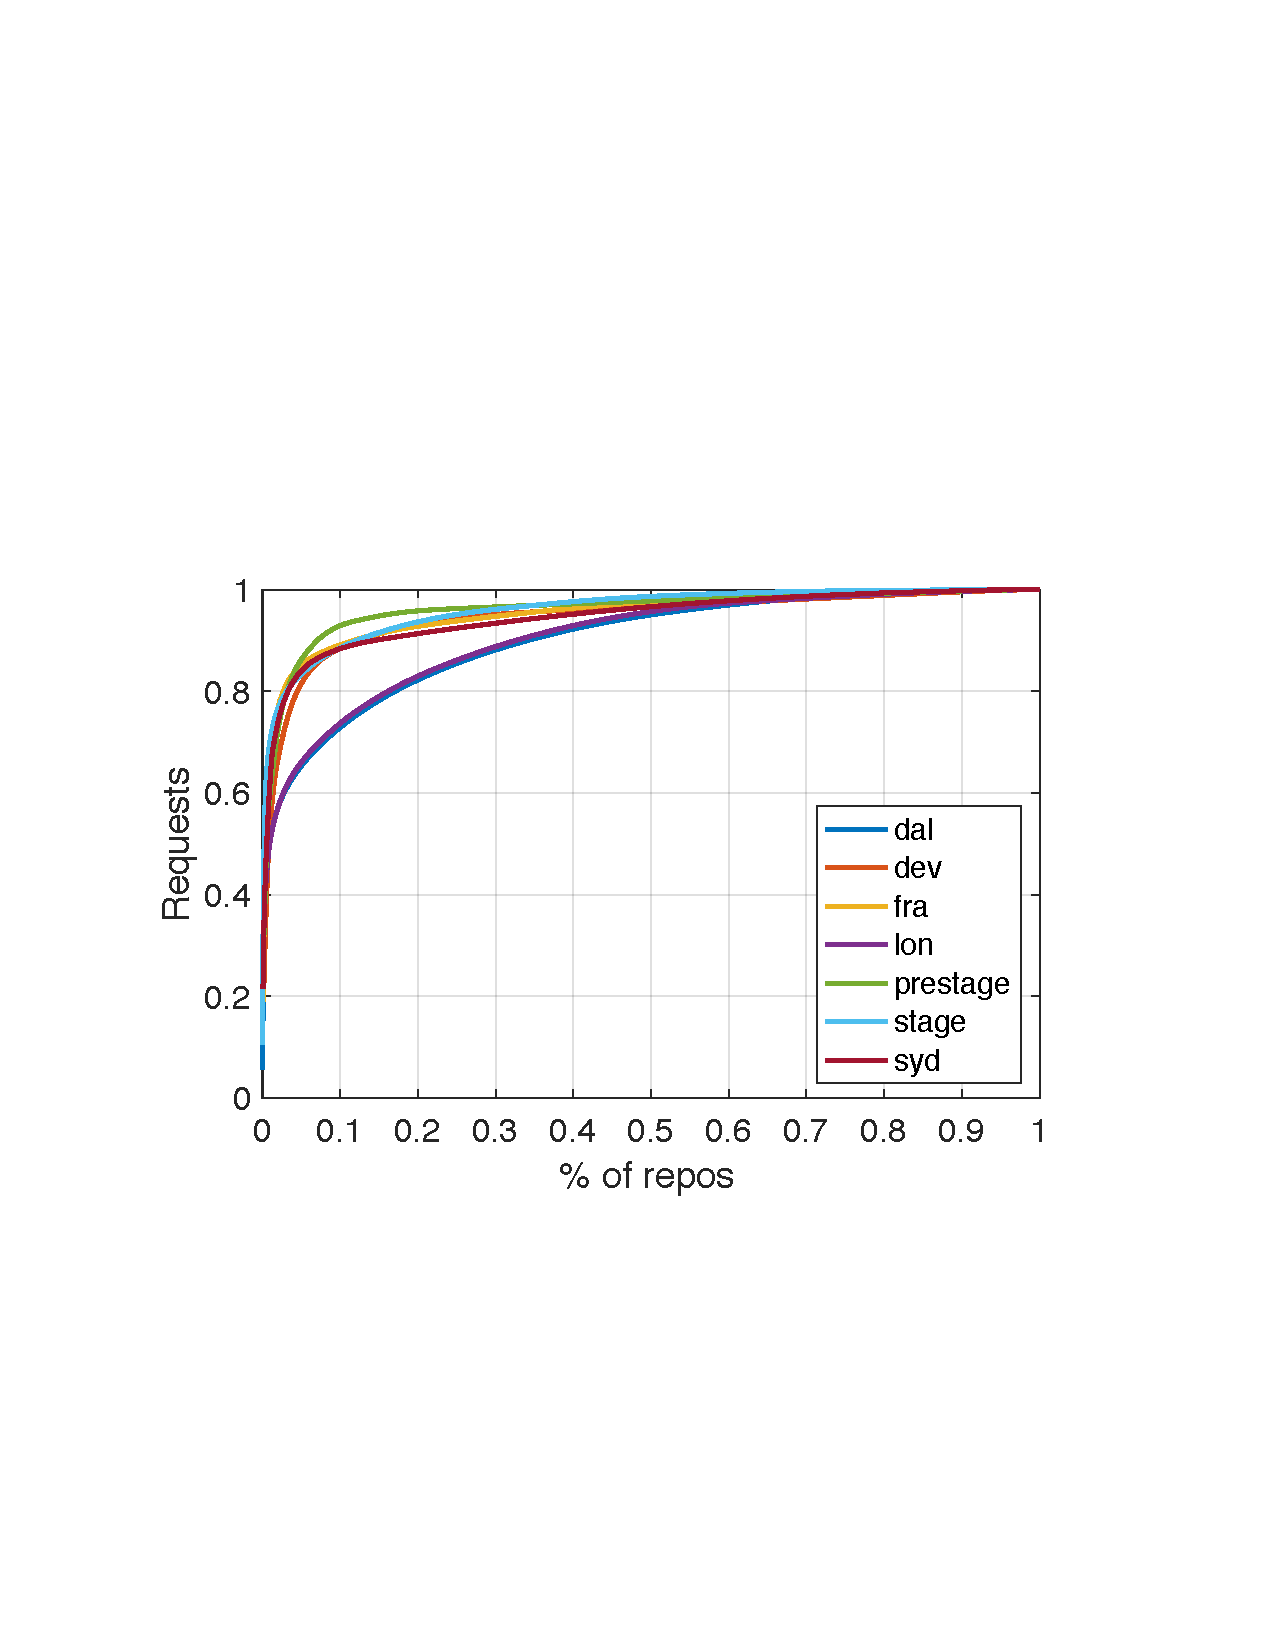
\includegraphics[width=0.2\linewidth]{graphs/repo-skewness.pdf}
		\label{fig:repo-skewness}
	}
	\subfigure[Client repulling probability]{
		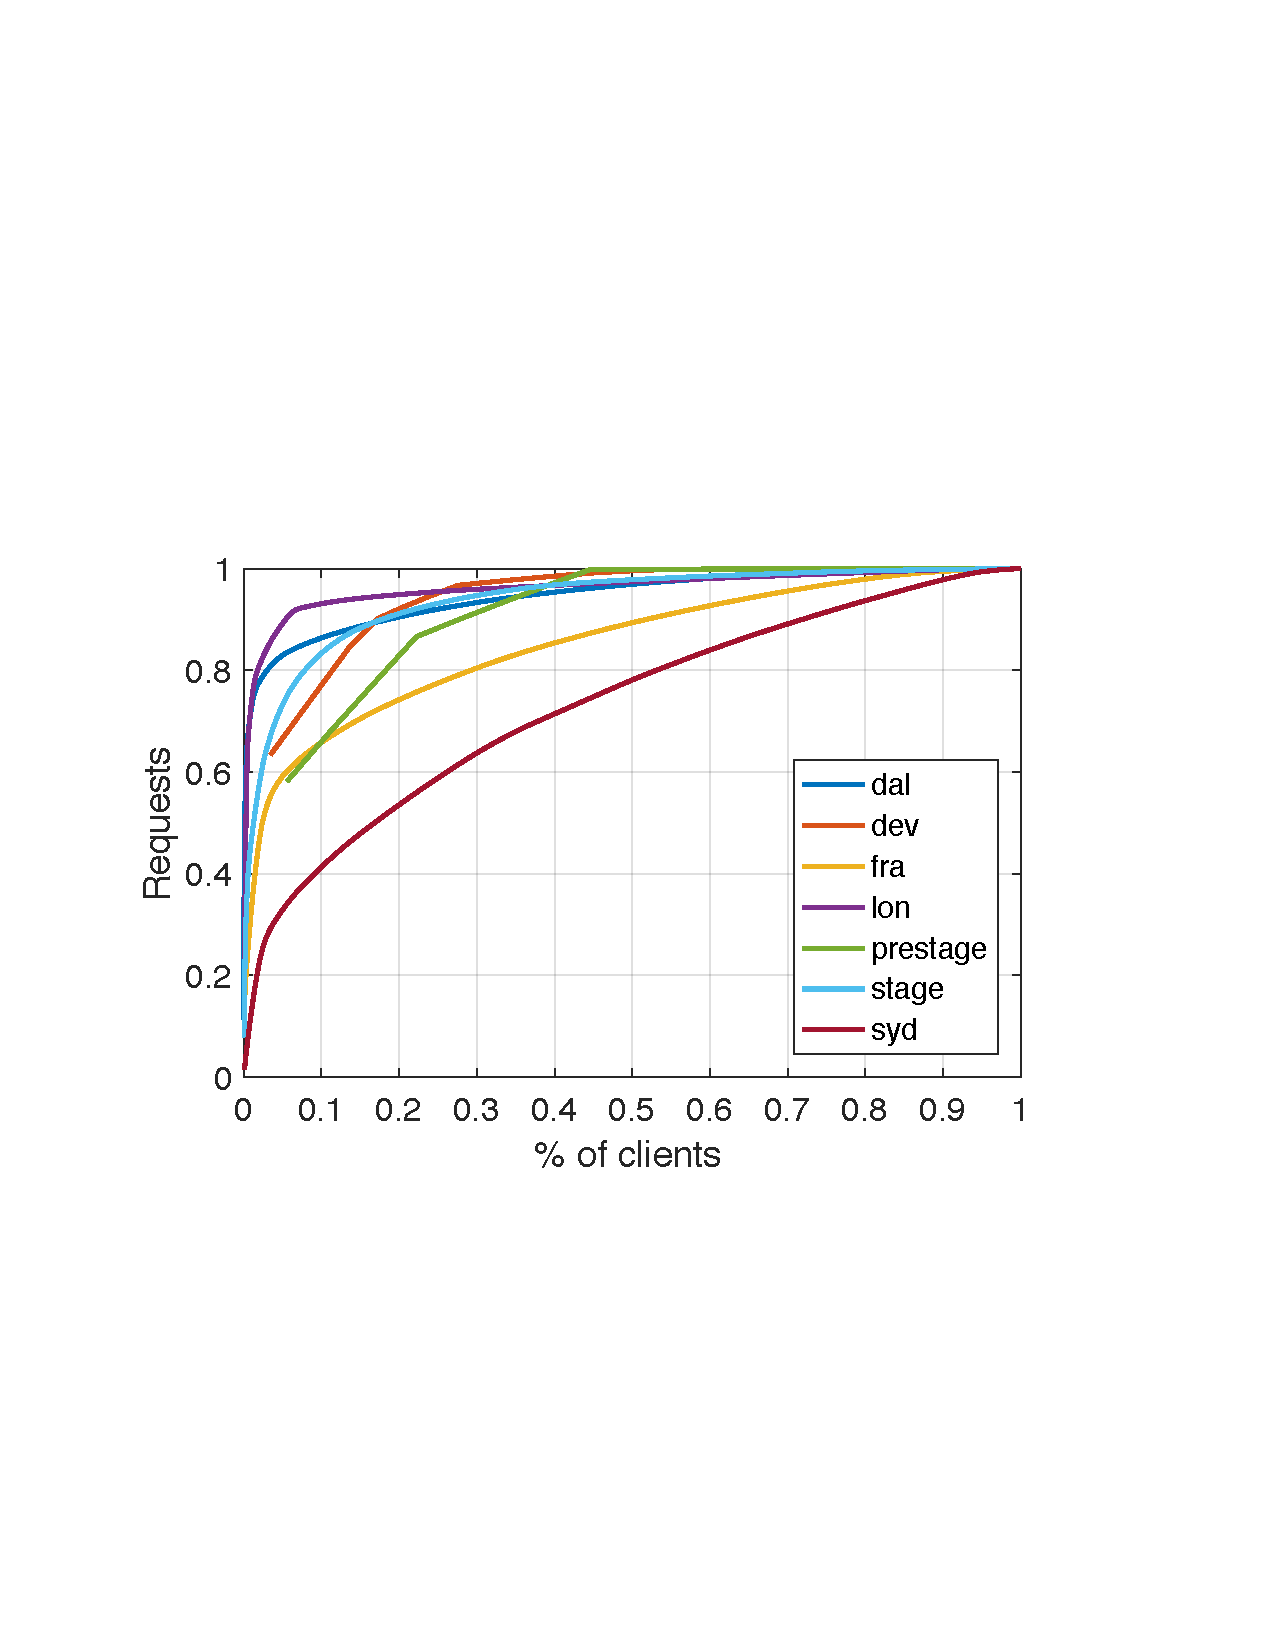
\includegraphics[width=0.2\linewidth]{graphs/client-skewness.pdf}
 	\label{fig:client-skewness}
	}
\caption{PDF of probability for layers, repositories, and clients.}
	\label{fig-skewness}
\end{figure*}
%=======
%\paragraph{User access patterns.} 
%
%\paragraph{Pull once VS. Always pull.}
%\HA{I think we should start the paragraph by stating that we are profiling users based on their behavior in repulling a repository and why}
%Figure~\ref{fig:layer-repull-cdf} shows the CDF of layer repull count. Here, \emph{repulling} indicates the act of pulling a layer that was previously pulled by the user because it is no longer present on the user's side.
%The majority of repulled layers are infrequently repulled.
%$83$\% of the repulled layers are only repulled twice.
%For example, only $3$\% of the layers from \texttt{Syd} are repulled more than twice.
%
%When different clients \texttt{pull} the same repository, 
%each client will only fetch, from the repository, the layers that are not present in their local layer dataset. Layers present locally on each client side vary with time as clients clear layer data. This makes clients pull different layers at different times.
%%they will fetch different amount of layers from the repository based on the contents of their local layer dataset. The local layers can vary with time due to clearing of the data so the same clients can fetch different amounts of layers at different times.
%Hence, a \texttt{pull manifest} request doesn't usually result in repulling all the layers in the repository. 
%Here, we define \emph{repulling a repository} as repulling the layers in the repository by the same client.
%Figure~\ref{fig:repo-repull-cdf} shows the CDF of the probability of repulling a repository, calculated by dividing the number of \texttt{pull manifest} requests resulting in repository repulls, by 
%the total number of \texttt{pull manifest} requests issued for the same repository.
%We see that the majority of repositories are not repulled.
%The percentage of repositories whose repull probability is zero (\ie are pulled only once by a client) ranges from $57$\% for \texttt{Prestage} to $85$\% for \texttt{Syd}.
%Only $20$\% of repositories from  \texttt{Prestage}, \texttt{Stage}, and 
%\texttt{Syd} have a repulling probability higher than $0.5$.
%We also observe that few repositories' repulling probability is $1$, indicating repulls everytime by the clients.
%
%Figure~\ref{fig:client-repull-cdf} shows the client repulling probability, calculated by dividing the number of \emph{repull} layer requests from a client, by
%the total number of \texttt{pull} layer requests issued by the same client.
%$60$\% of clients from \texttt{Prestage}, \texttt{Dev}, \texttt{Lon}, and \texttt{Fra} have a repulling probability lower than $0.1$.
%$2$\%-$12$\% of clients have a repulling probability higher than $0.9$ from workloads:
%\texttt{Dal}, \texttt{Dev}, \texttt{Fra}, \texttt{Prestage},
%\texttt{Stage}, \texttt{Syd}, and \texttt{Lon}.
%
%From the probability distribution of the clients repulling, we can observe that a significant chunk of the clients %are rarely repulling a repository
% have a very low repulling probability and another chunk of the clients have a very high repulling probability, with few clients in the middle. For simplicity of implementation, the high probability clients can be classified as always repulling clients, and the low probability clients as never repulling (i.e. they pull only once). The few clients in the middle are considered erratic  and no classification is made for them.
%
%
%
%\subsection{Temporal Access Patterns}
%%\begin{figure*}[t]
%		\begin{minipage}{0.32\linewidth}
%			\centering
%			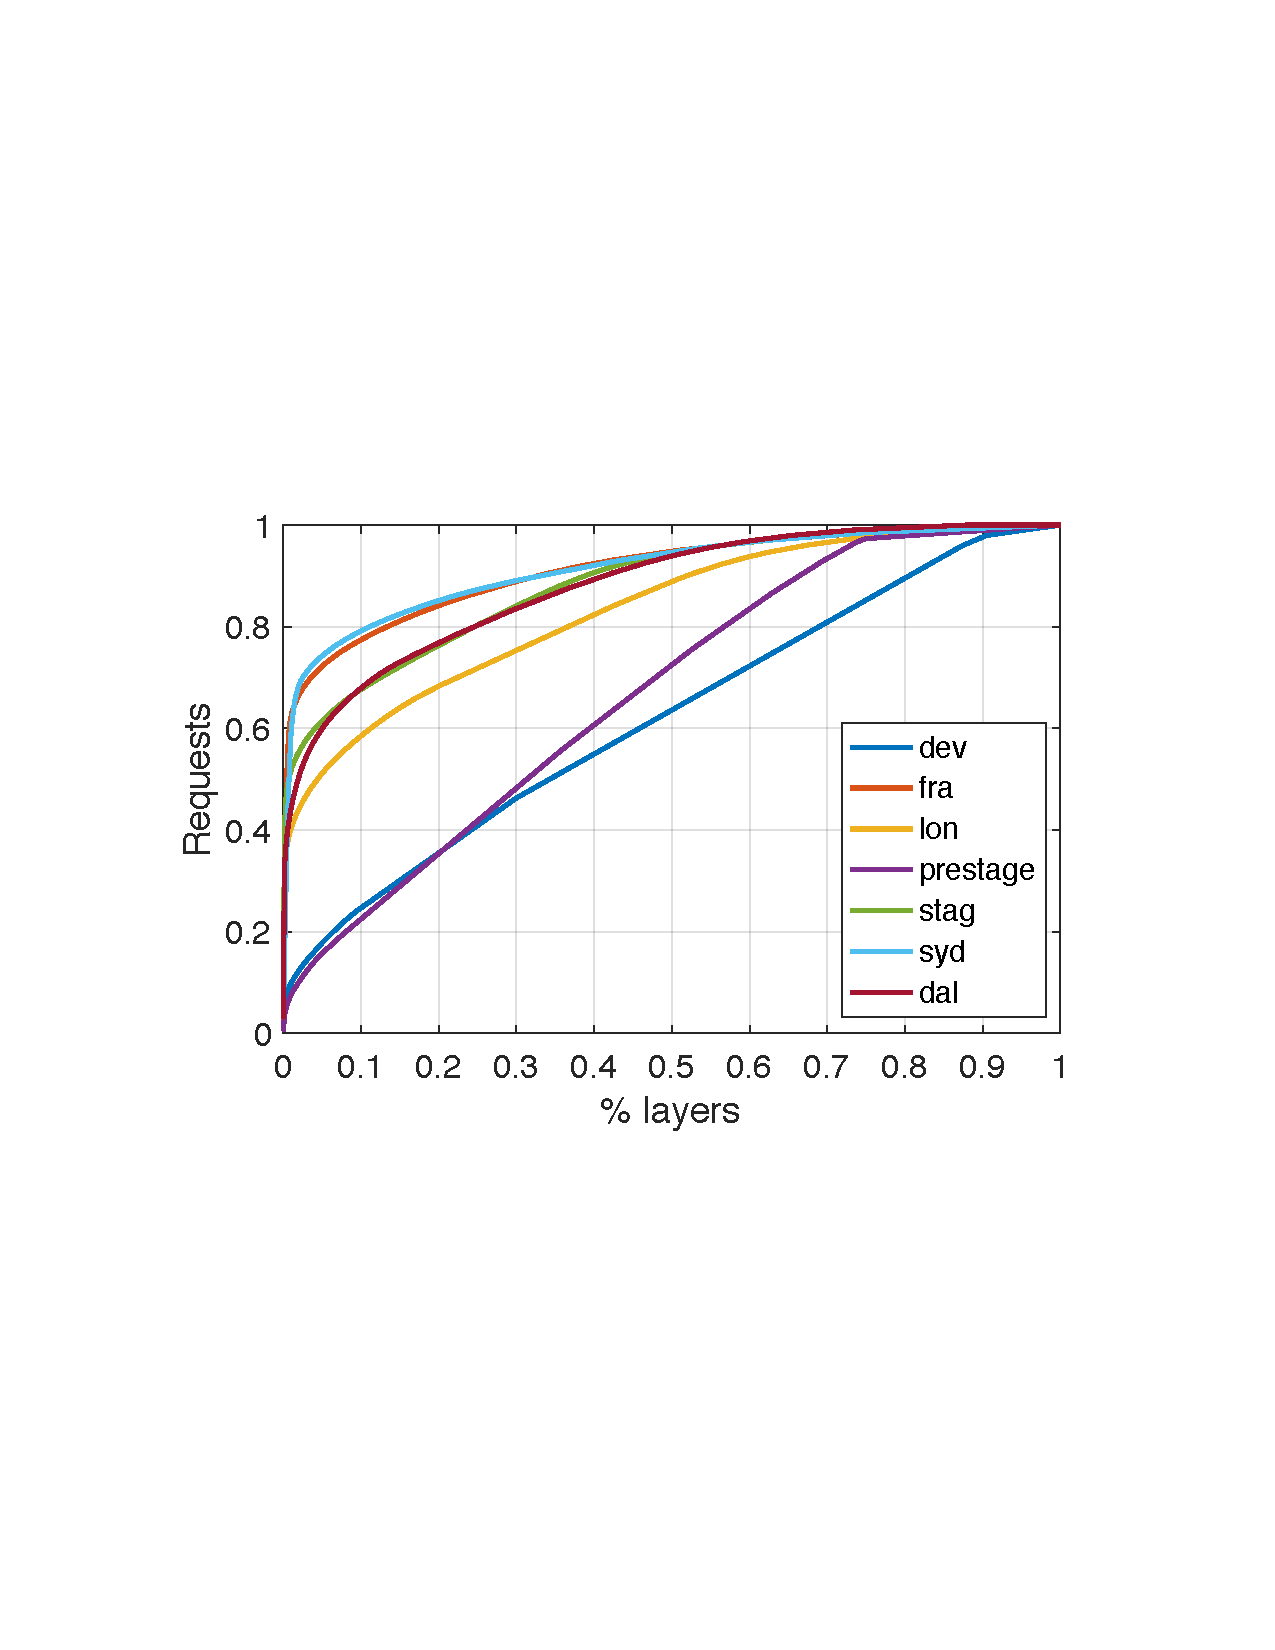
\includegraphics[width=1\textwidth]{graphs/layer_skewness.pdf}
%			%\caption{CDF of layer  count.}
%		%	\vspace{-3pt}
%			\label{fig:layer-skenwess}
%		\end{minipage}
%			\begin{minipage}{0.32\linewidth}
%				\centering
%				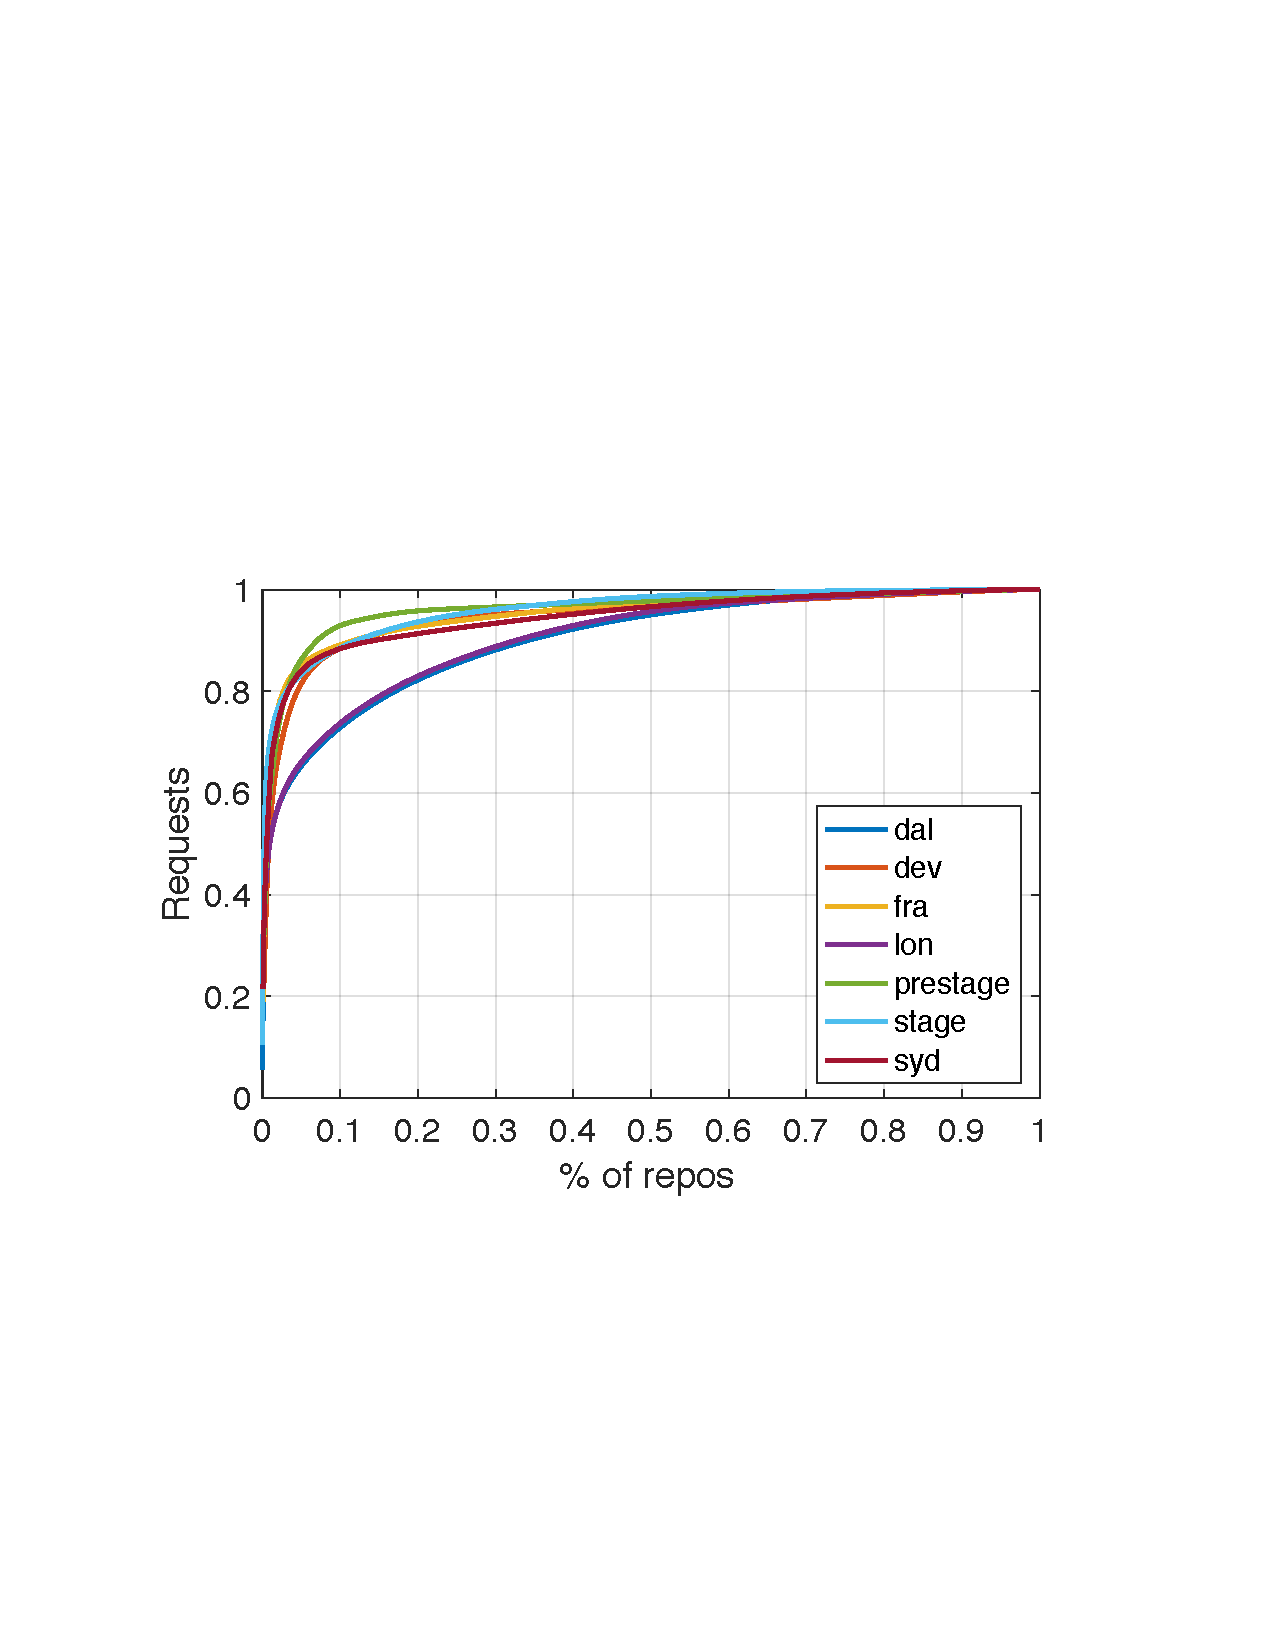
\includegraphics[width=1\textwidth]{graphs/repo-skewness.pdf}
%				%\caption{PDF of repository repulling probability.}
%				%	\vspace{-3pt}
%				\label{fig:repo-skewness}
%			\end{minipage}
%		\hfill
%		\begin{minipage}{0.32\linewidth}
%			\centering
%			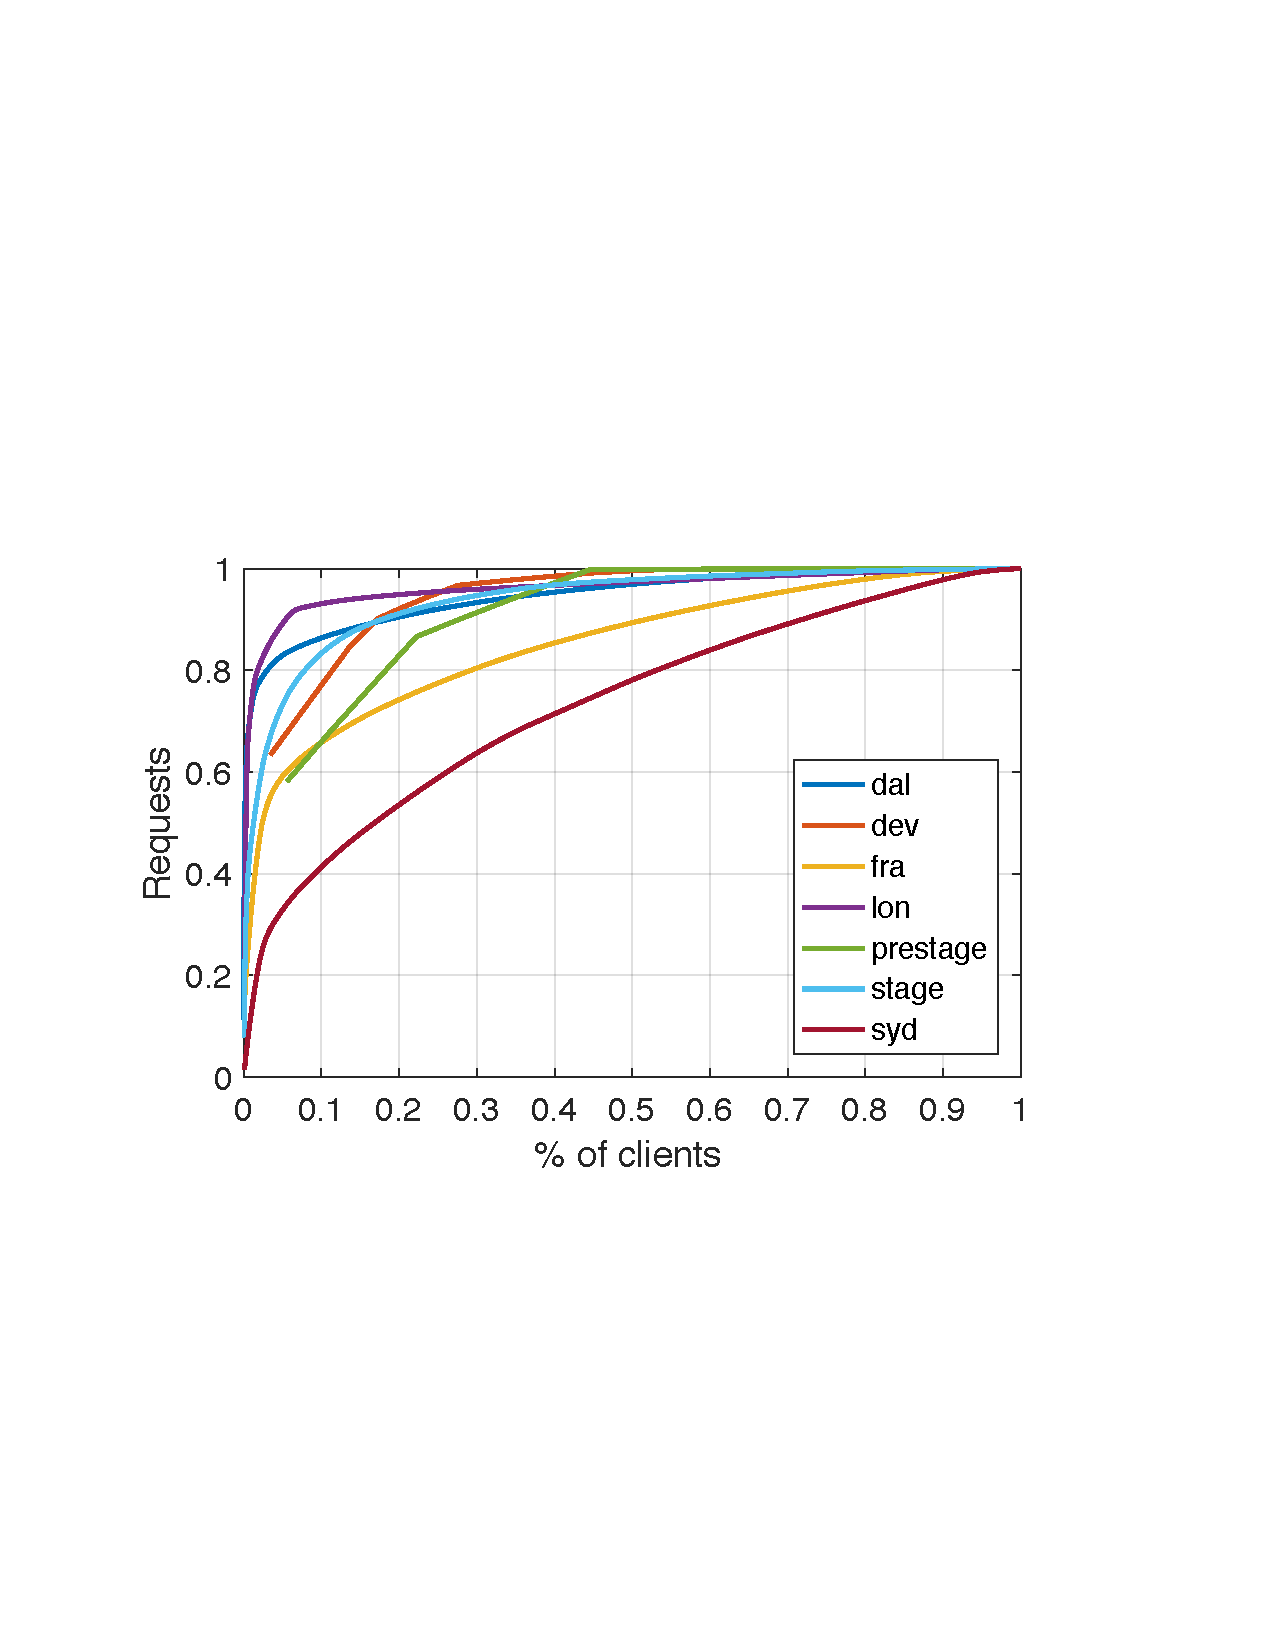
\includegraphics[width=1\textwidth]{graphs/client-skewness.pdf}
%			%\caption{PDF of client repulling probability.}
%			%	\vspace{-3pt}
%			\label{fig:client-skewness}
%			
%		\end{minipage}
%\caption{PDF of probability for layers, repositories, and clients.}
%%	\label{}
%\end{figure*}

\begin{figure*}[!t]
	\centering
	\subfigure[Layer repull count]{
		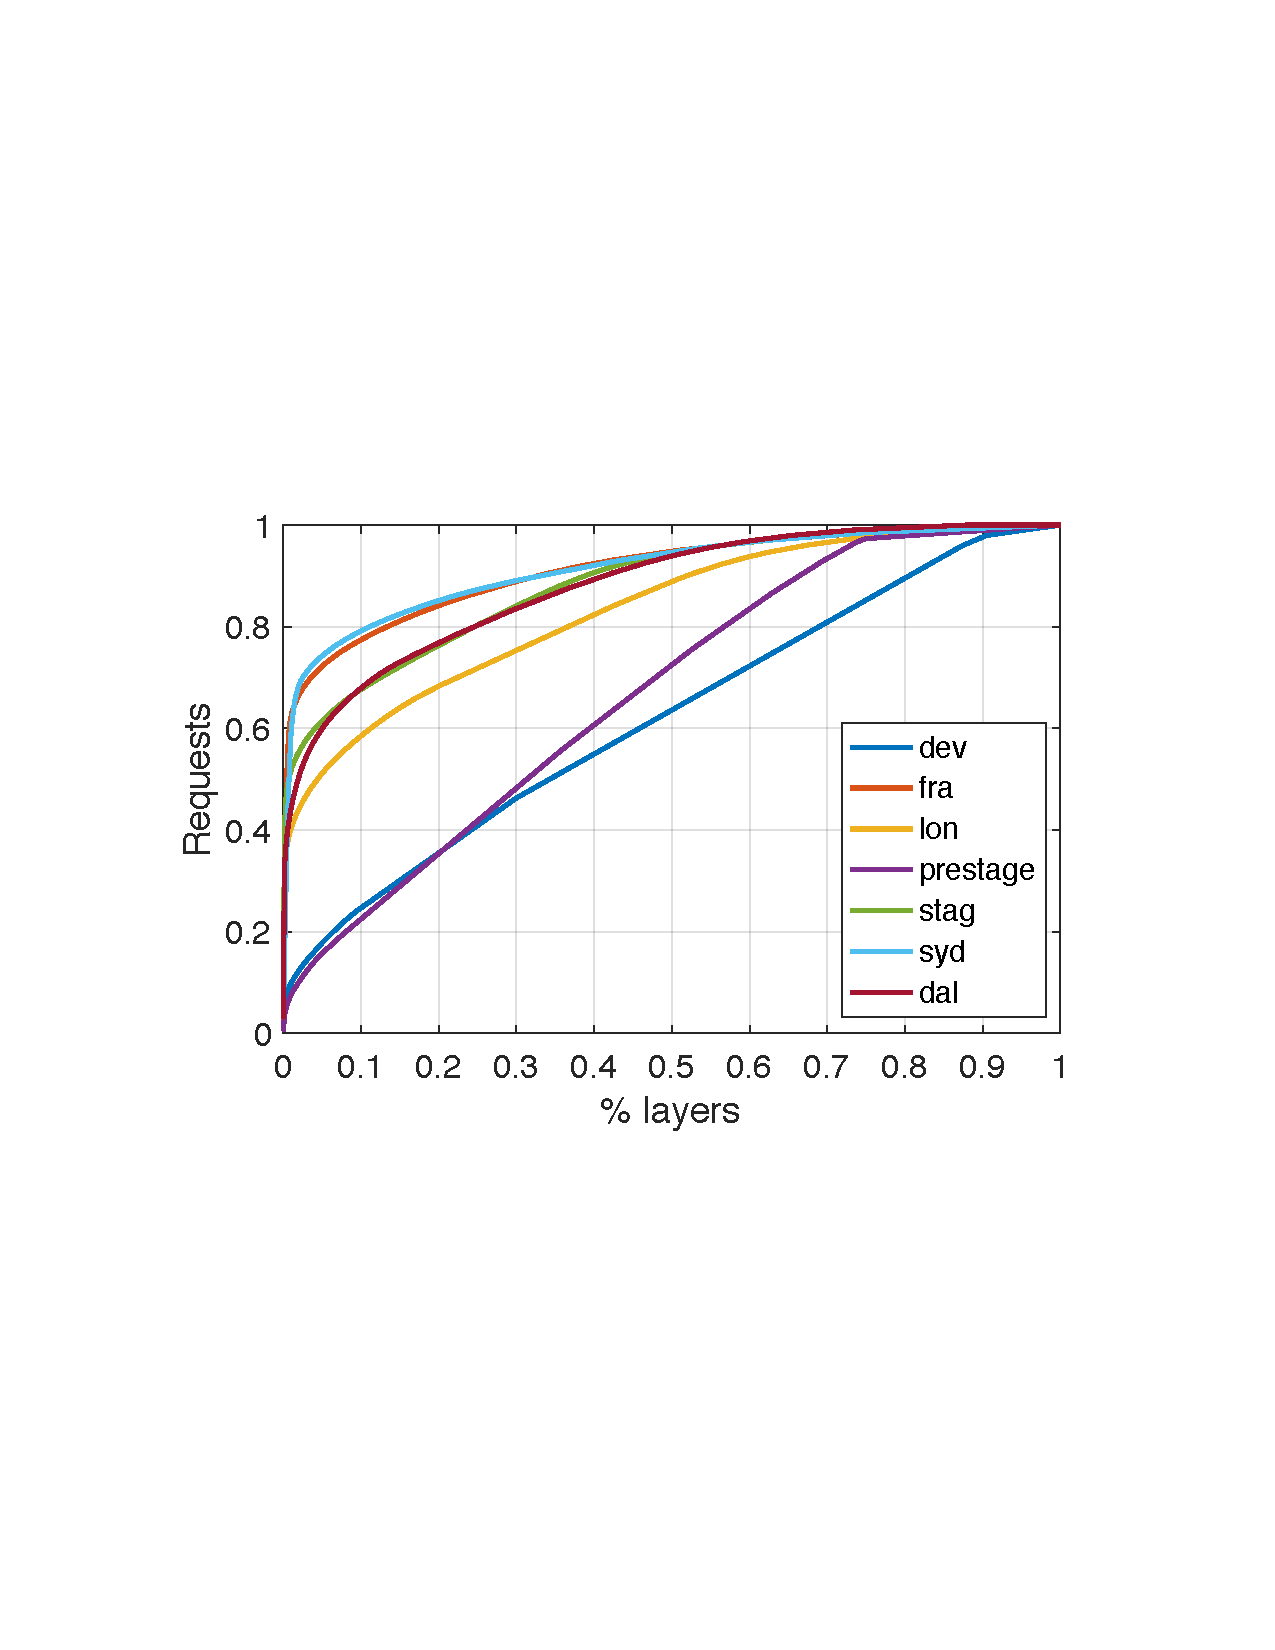
\includegraphics[width=0.2\linewidth]{graphs/layer_skewness.pdf}
		\label{fig:layer-skenwess}
	}
	\subfigure[Repository repulling probability]{
		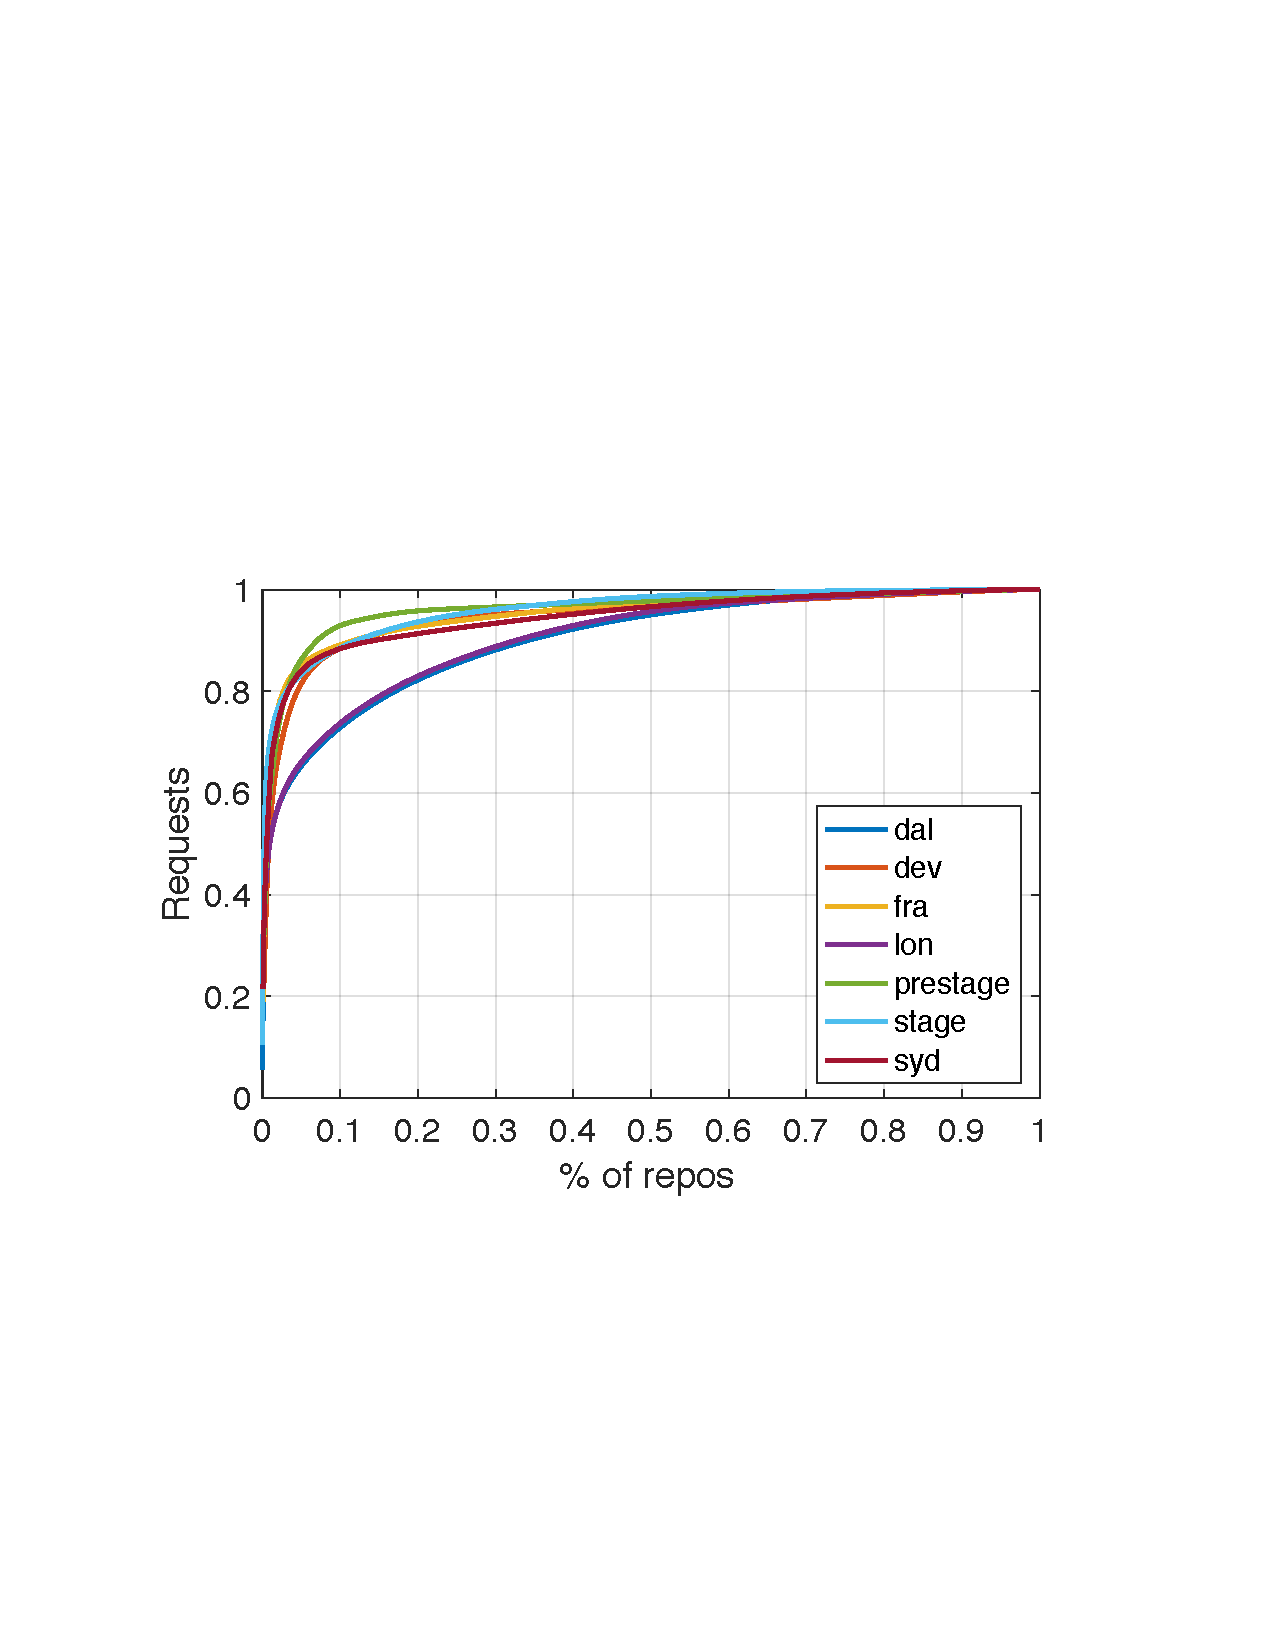
\includegraphics[width=0.2\linewidth]{graphs/repo-skewness.pdf}
		\label{fig:repo-skewness}
	}
	\subfigure[Client repulling probability]{
		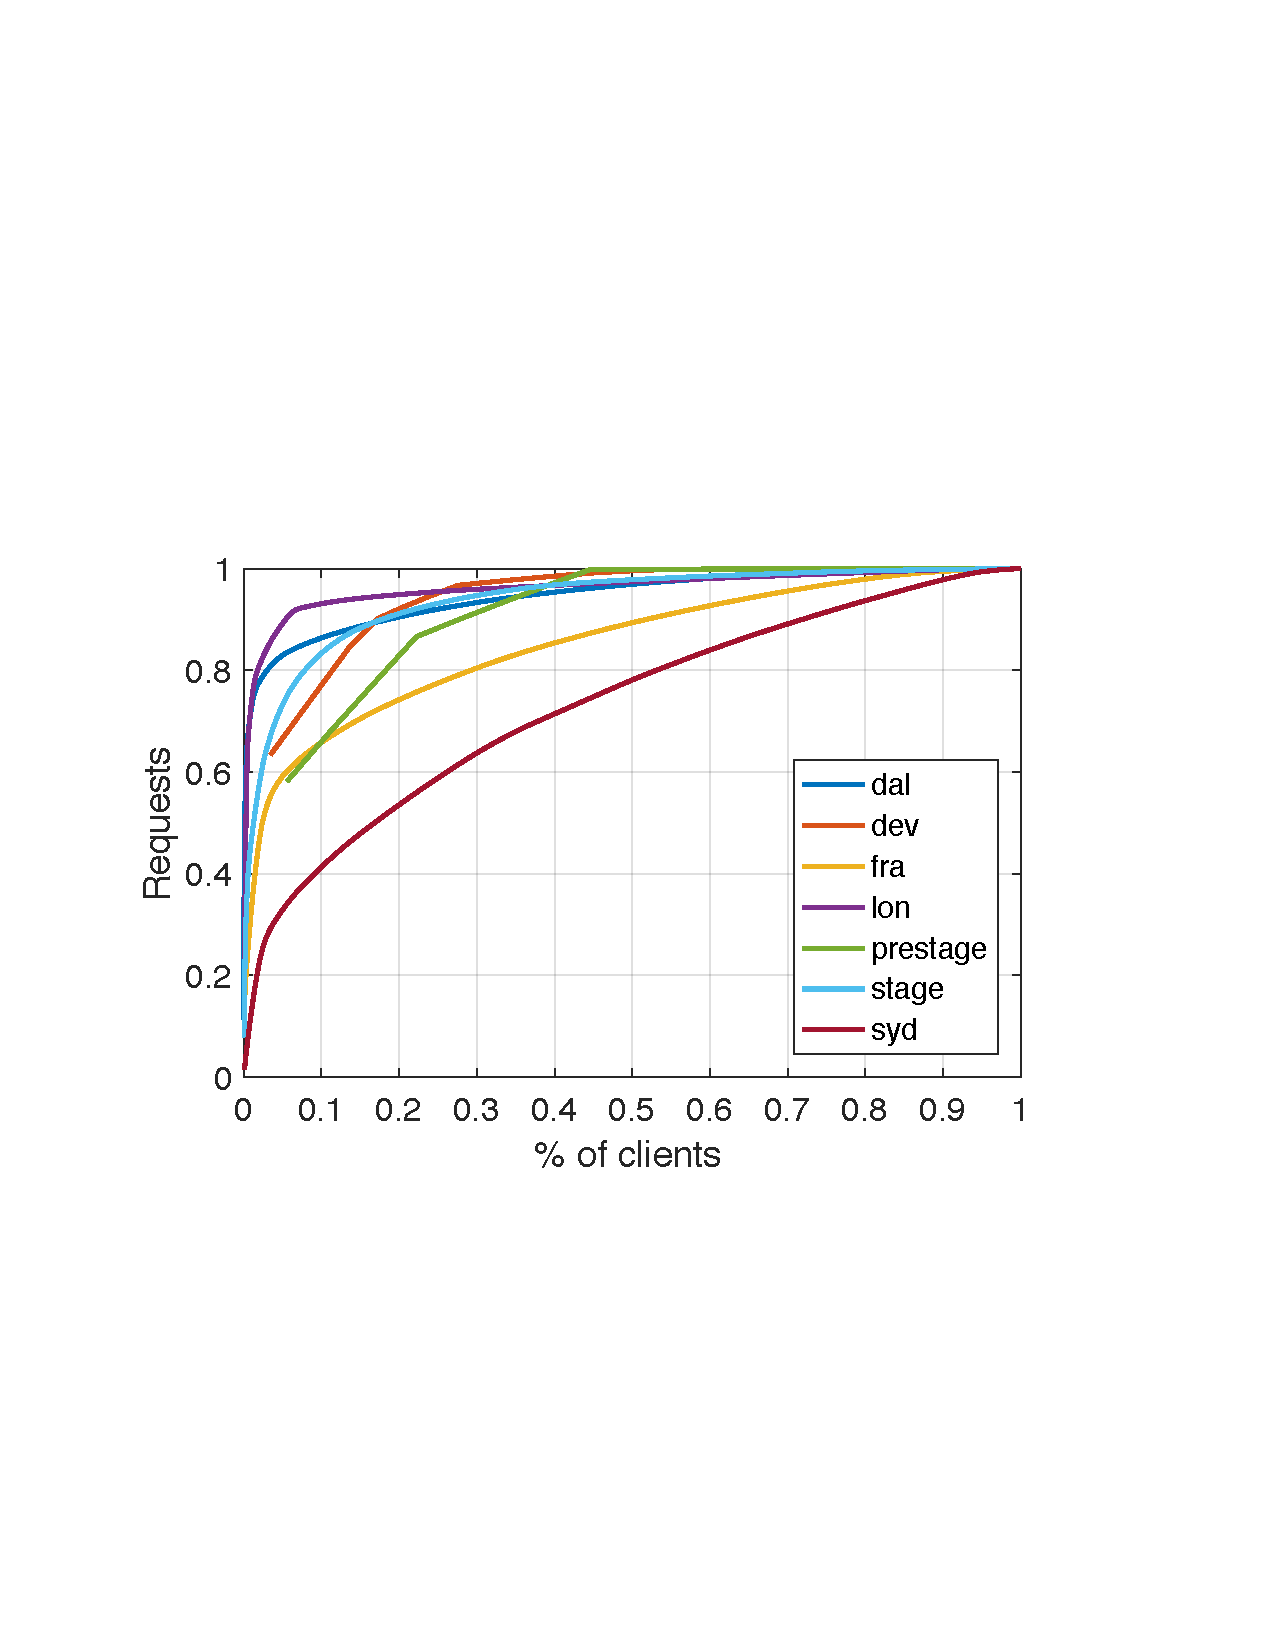
\includegraphics[width=0.2\linewidth]{graphs/client-skewness.pdf}
 	\label{fig:client-skewness}
	}
\caption{PDF of probability for layers, repositories, and clients.}
	\label{fig-skewness}
\end{figure*}
%>>>>>>> 94daa3df1d5d977ac11fd9da2aea7b4eed340be2
%\begin{figure*}[t]
%		\begin{minipage}{0.32\linewidth}
%			\centering
%			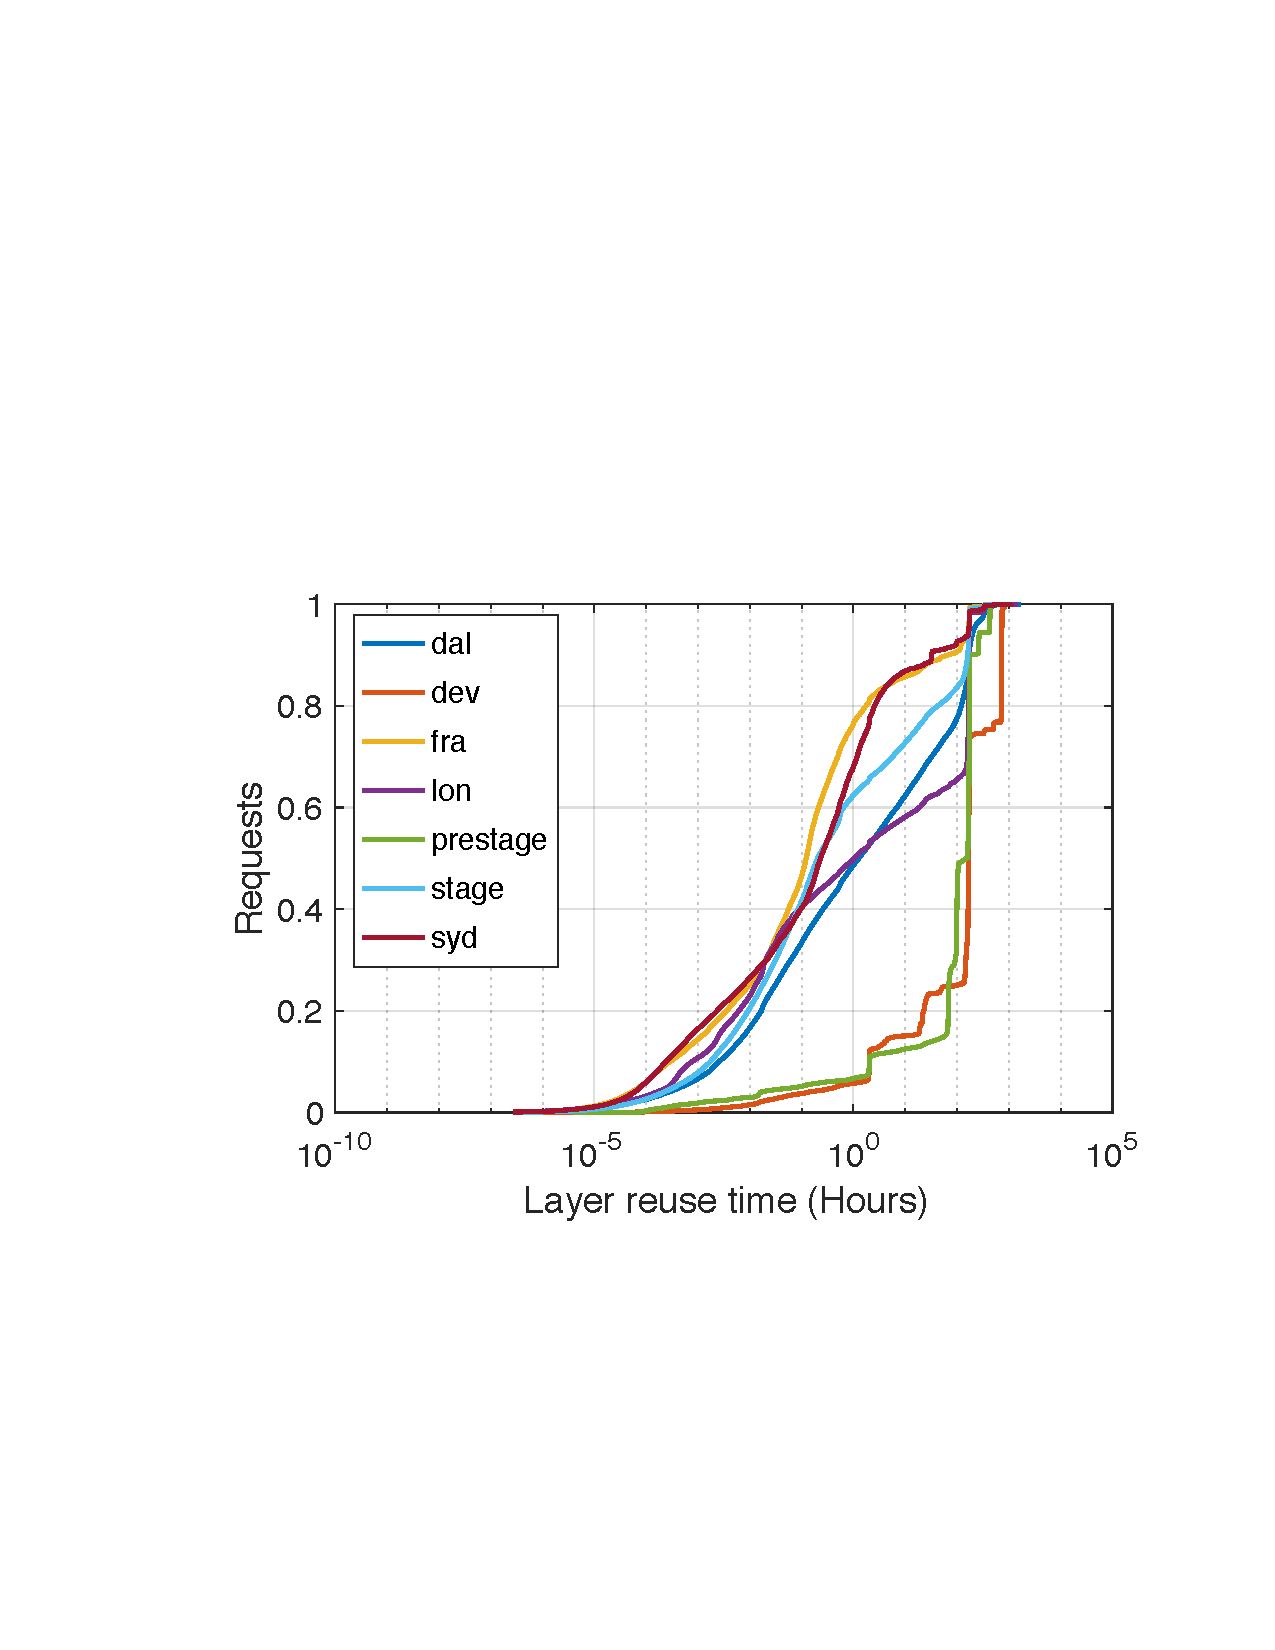
\includegraphics[width=1\textwidth]{graphs/layer-reusetime.pdf}
%		%	\caption{CDF of layer reuse time.}
%		%	\vspace{-3pt}
%			\label{fig:layer-reuse}
%		\end{minipage}
%			\begin{minipage}{0.32\linewidth}
%				\centering
%				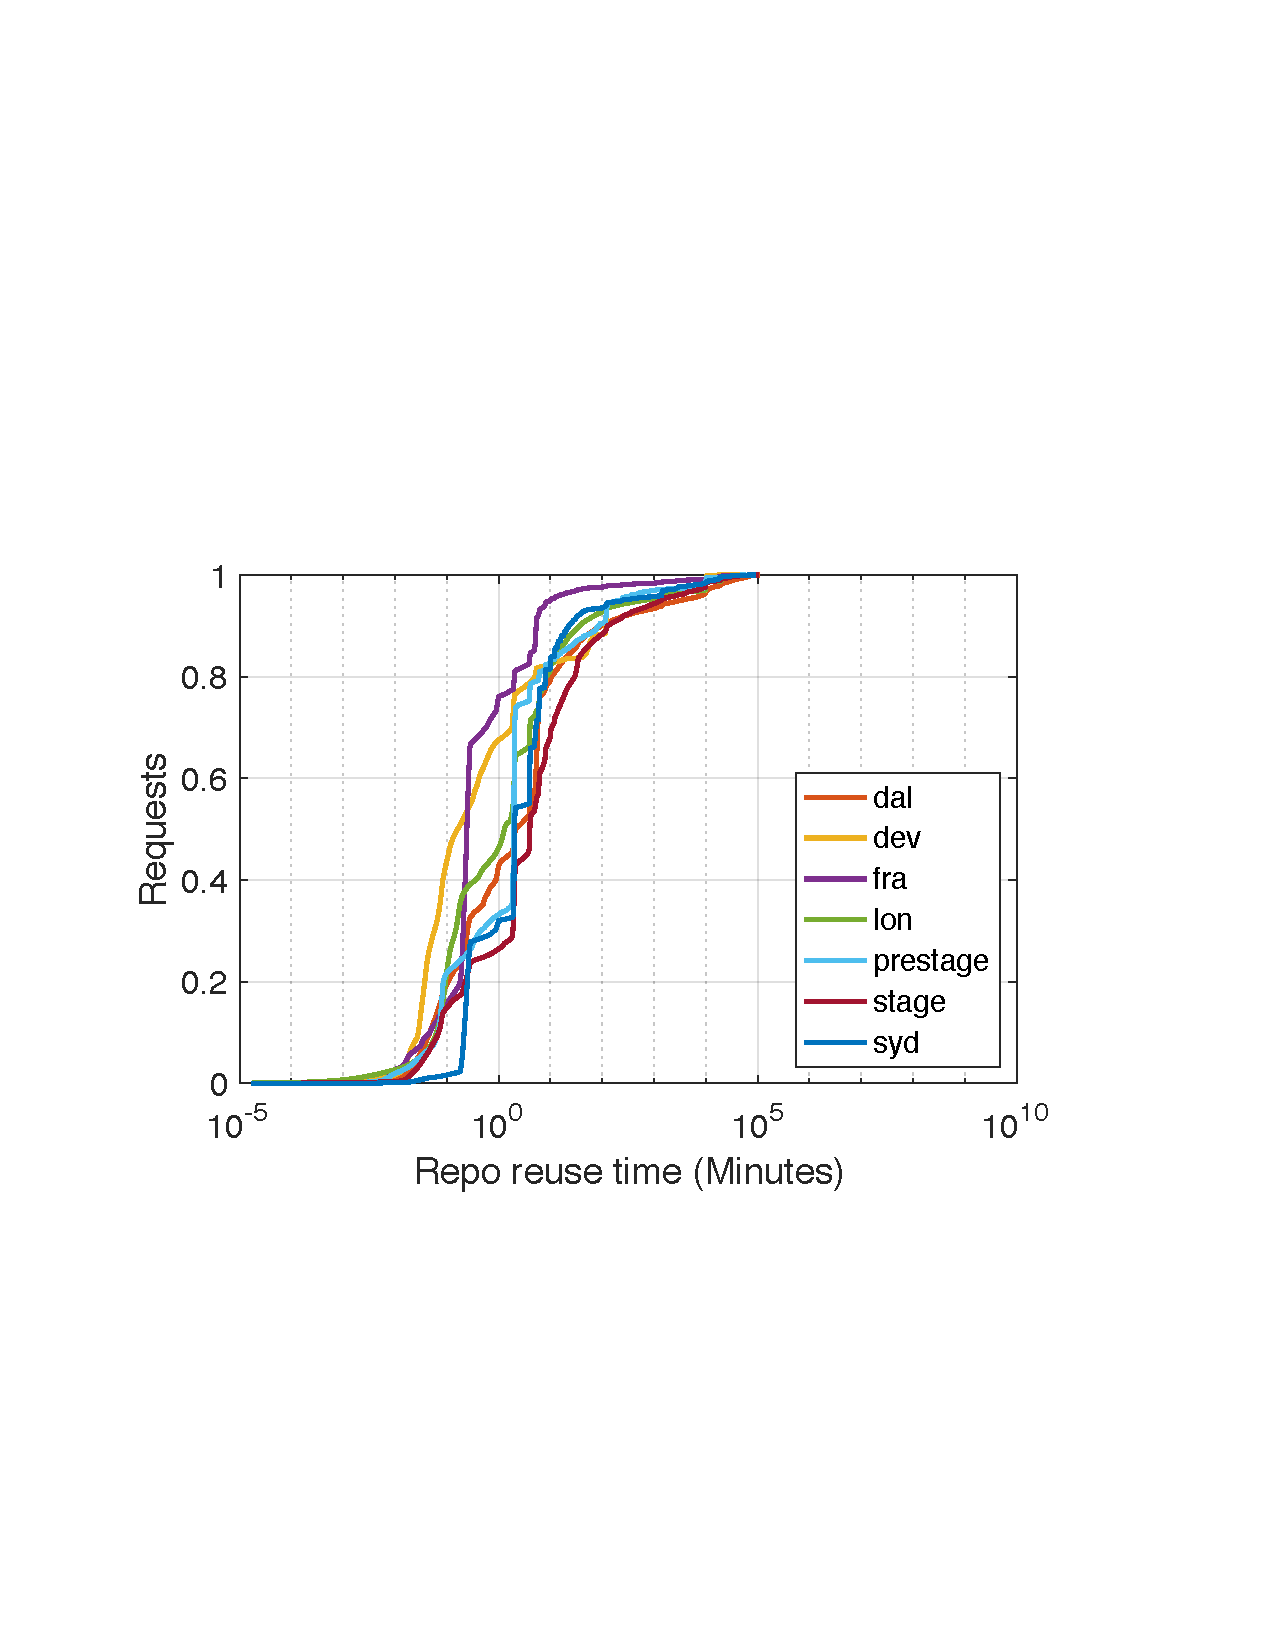
\includegraphics[width=1\textwidth]{graphs/repo-reusetime.pdf}
%			%	\caption{PDF of repository reuse time.}
%				%	\vspace{-3pt}
%				\label{fig:repo-reuse}
%			\end{minipage}
%		\begin{minipage}{0.32\linewidth}
%			\centering
%			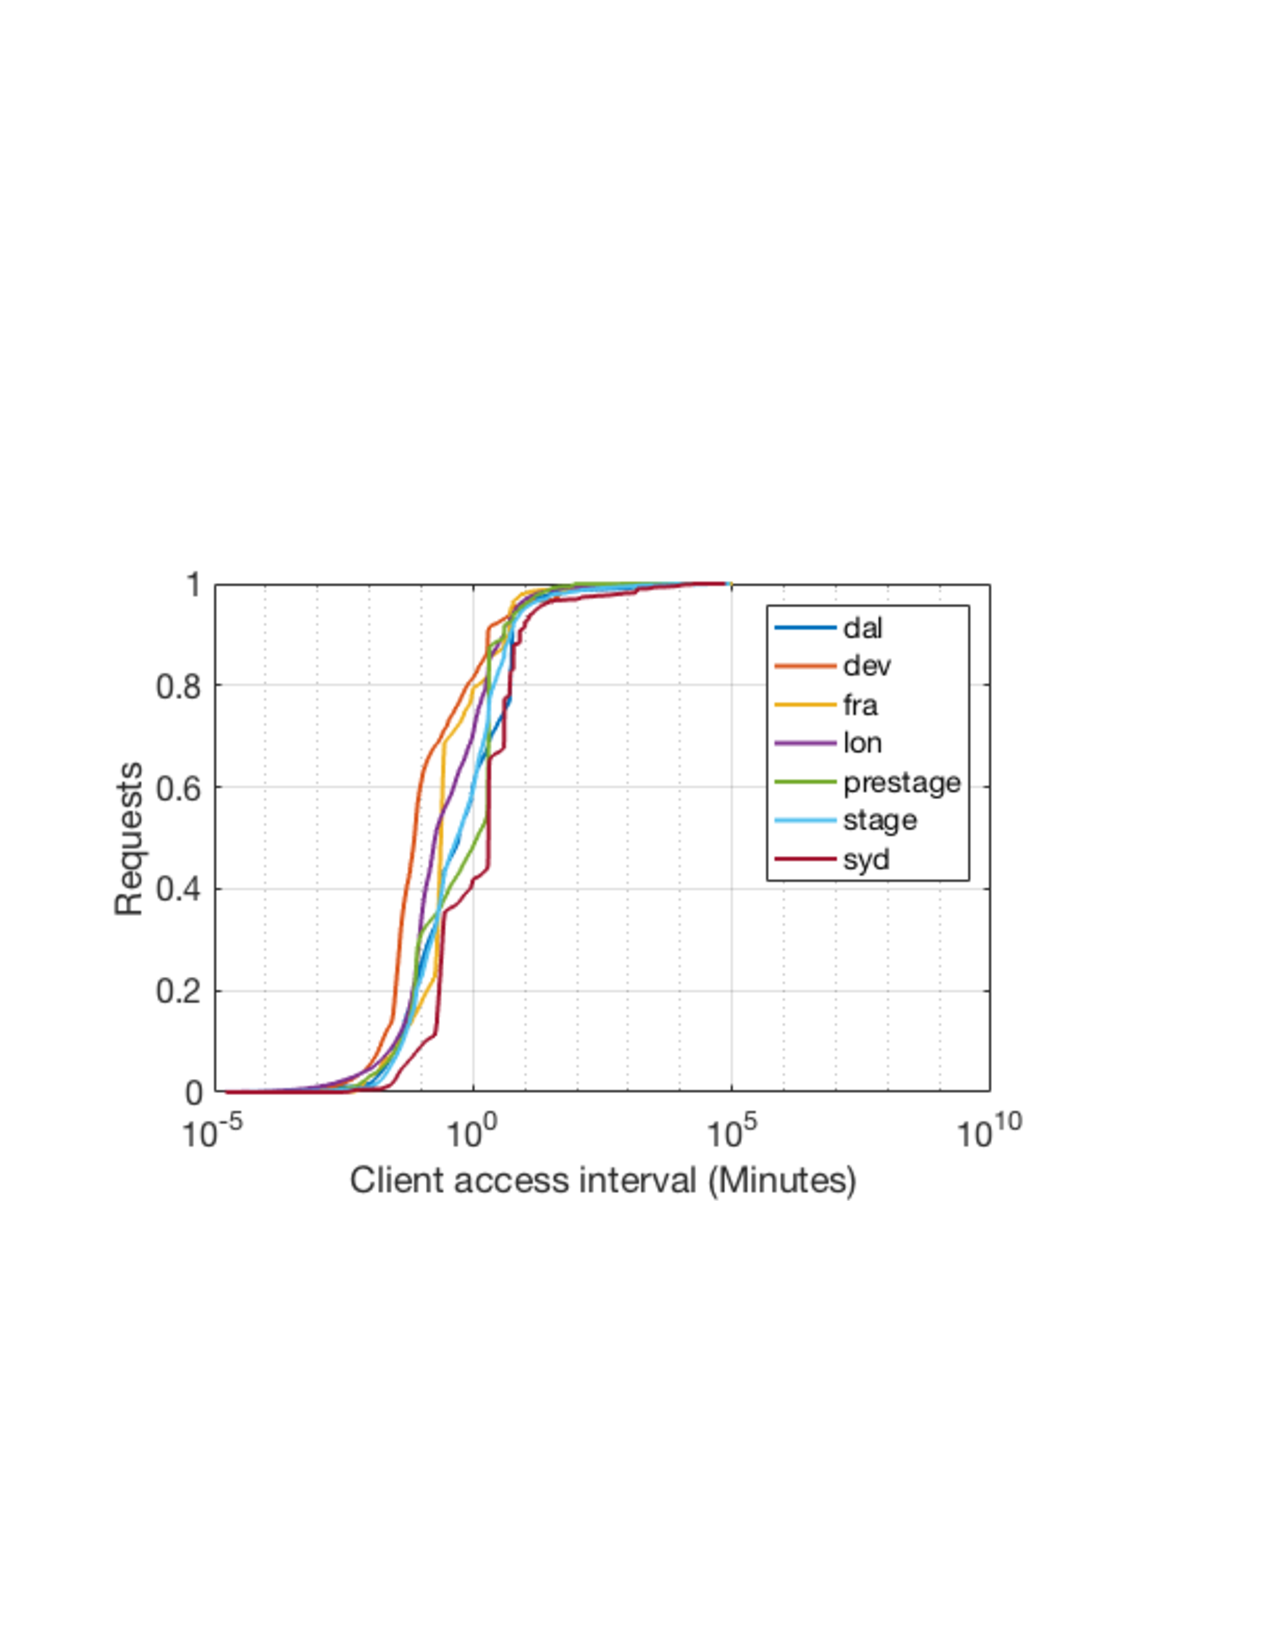
\includegraphics[width=1\textwidth]{graphs/user-intervals.pdf}
%			%\caption{PDF of client access intervals.}
%			%	\vspace{-3pt}
%			\label{fig:user-interval}
%		\end{minipage}
%	\caption{CDF of reusetime for layers, repositories and clients' access intervals.}
%	\label{fig:layer-reuse}
%\end{figure*}
\begin{figure}[t]
	\centering
	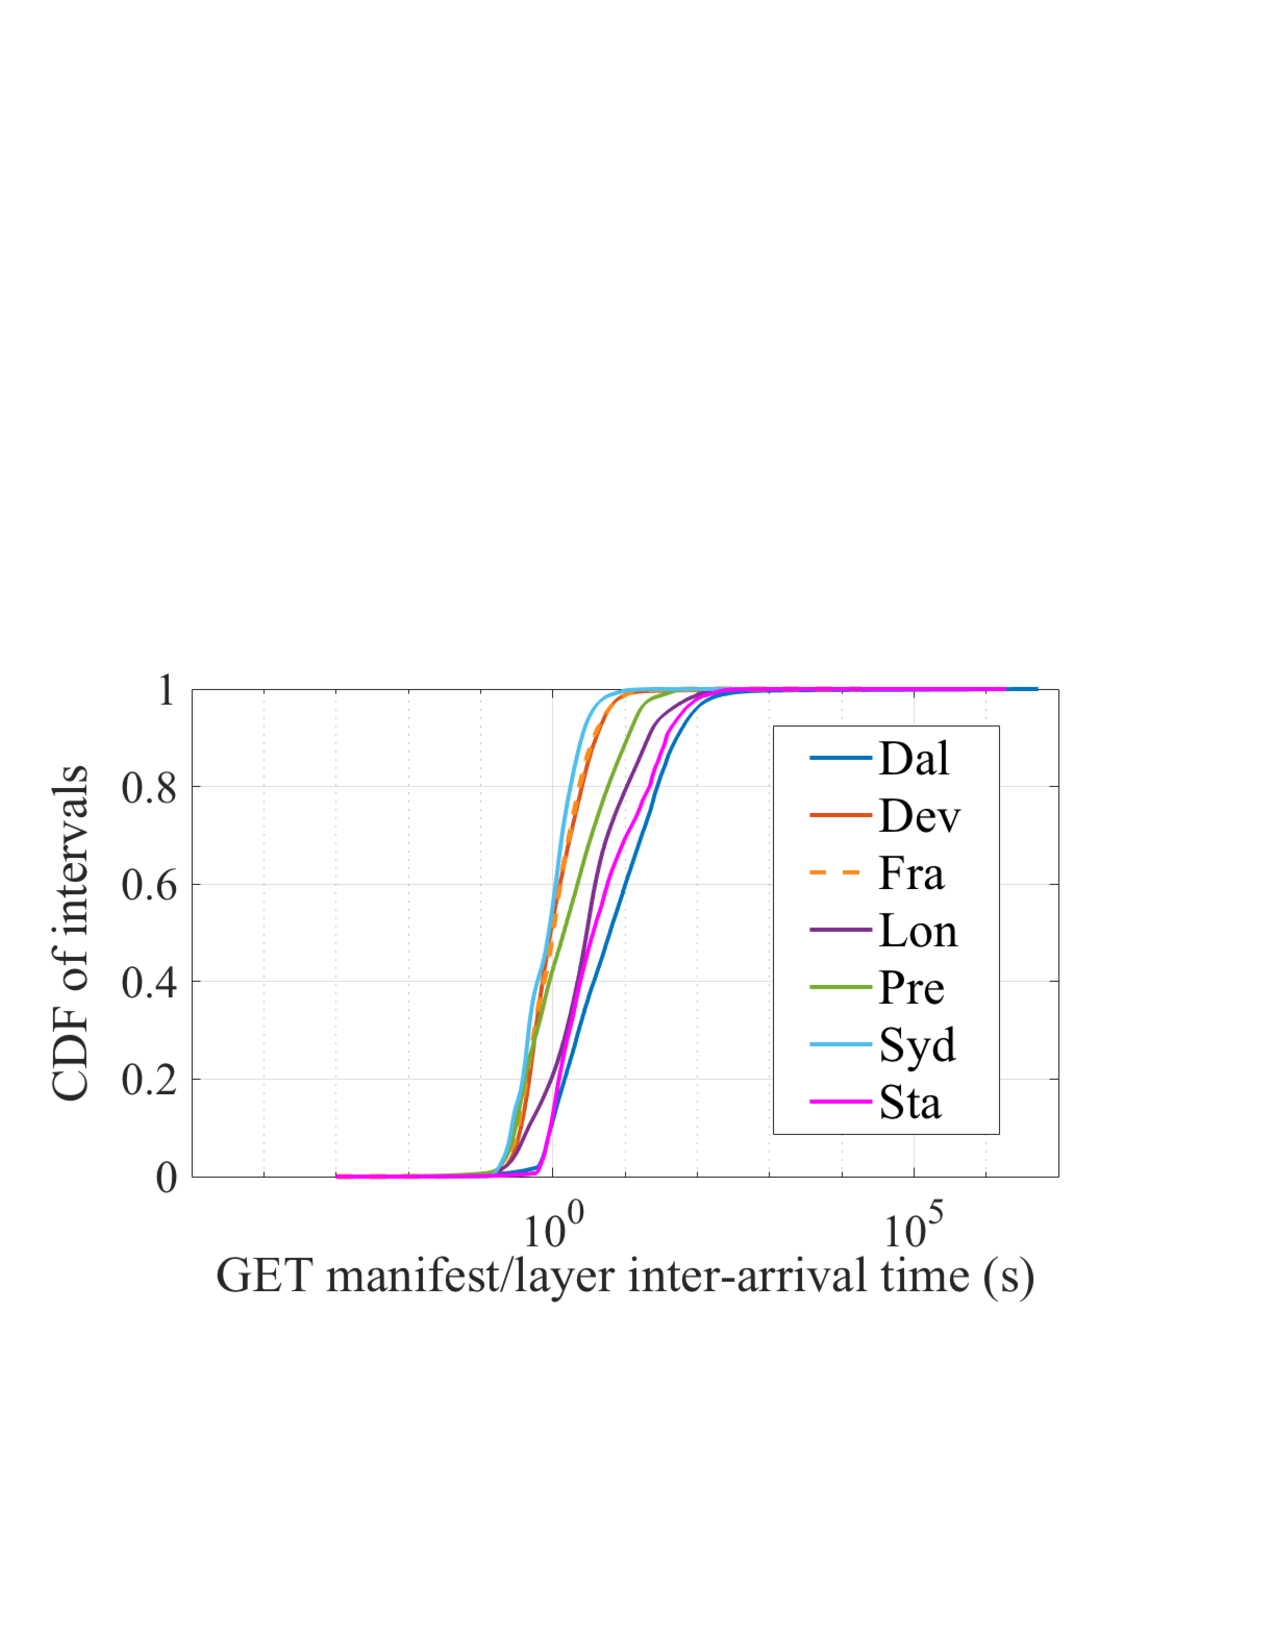
\includegraphics[width=0.3\textwidth]{graphs/GML-intervals.pdf}
	\caption{Intervals between \texttt{pull} manifest request and \texttt{pull} layer request}
	%	\vspace{-3pt}
	\label{fig:intervals}
	
\end{figure}
%\begin{figure*}[!t]
%	\centering
%	\subfigure[Layer repull count]{
%		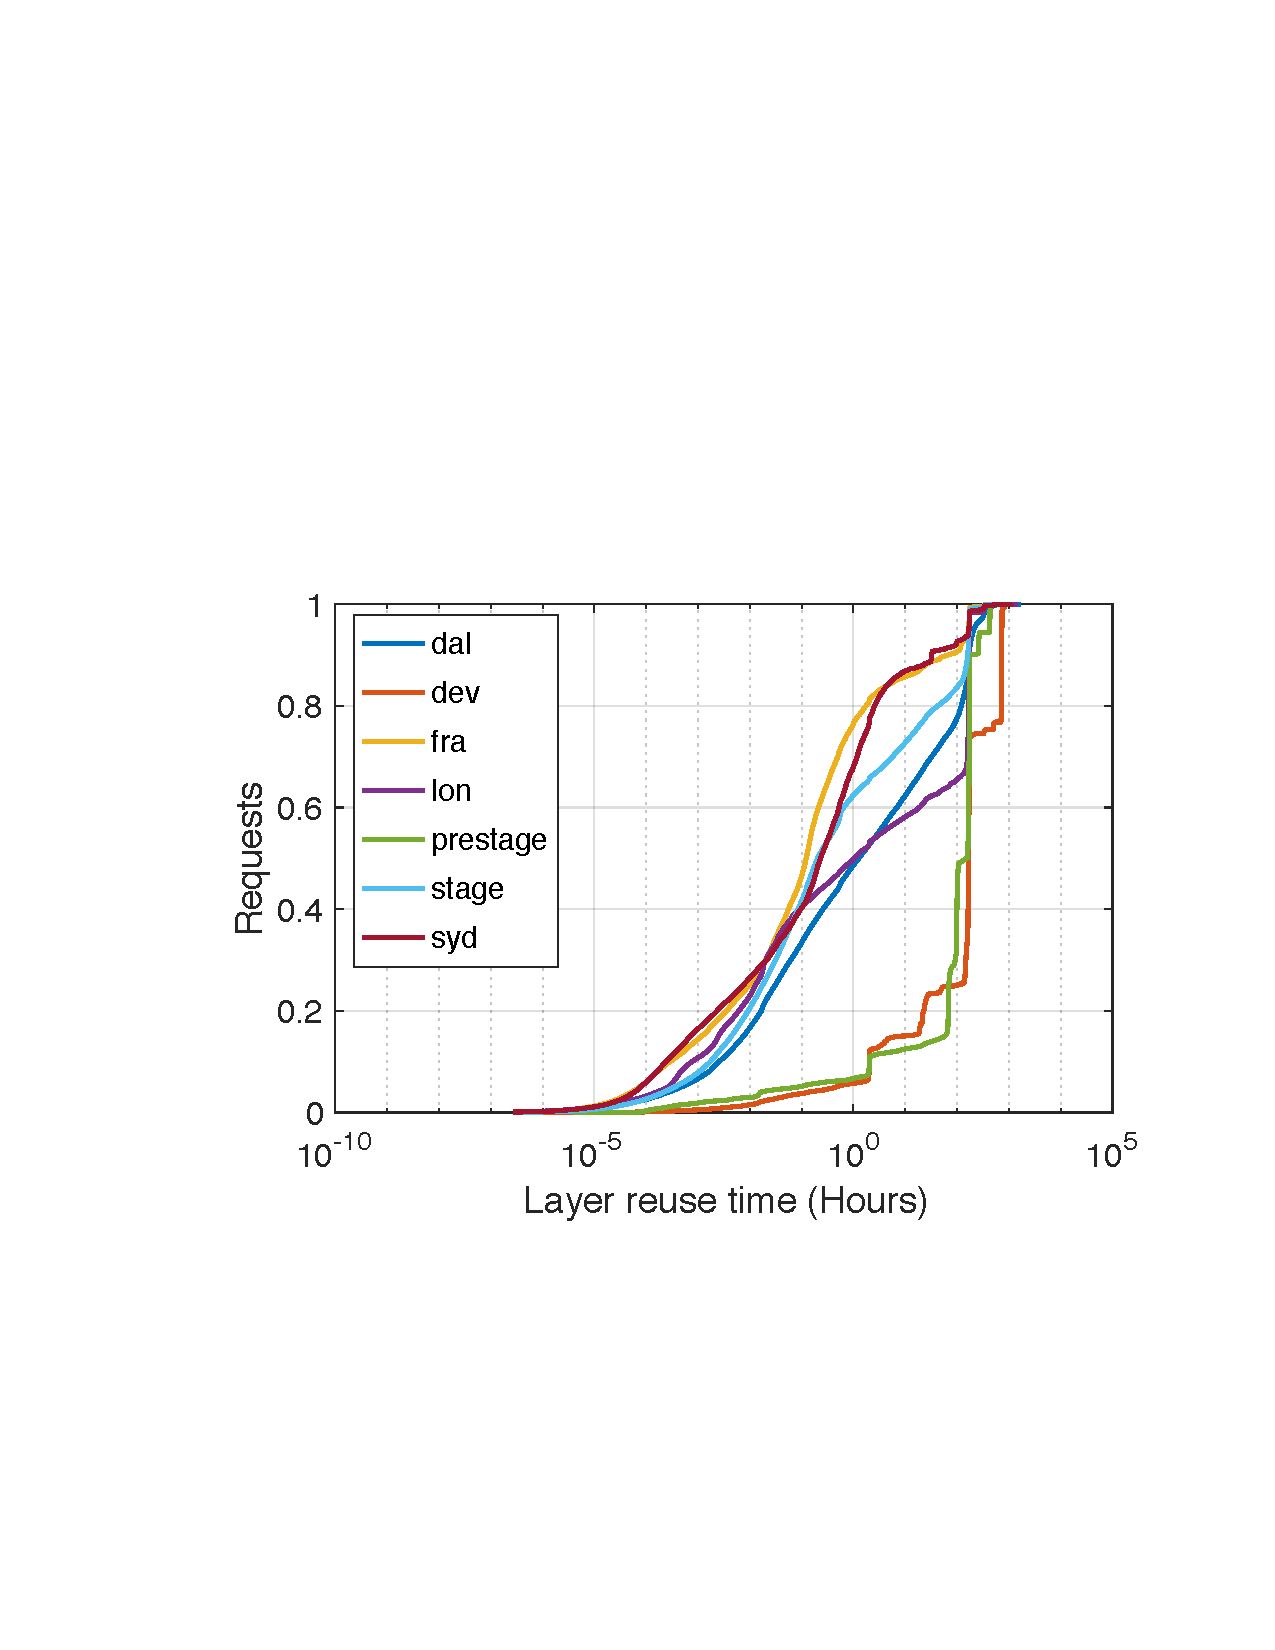
\includegraphics[width=0.2\linewidth]{graphs/layer-reusetime.pdf}
%			\label{fig:layer-reuse}
%	}
%	\subfigure[Repository repulling probability]{
%		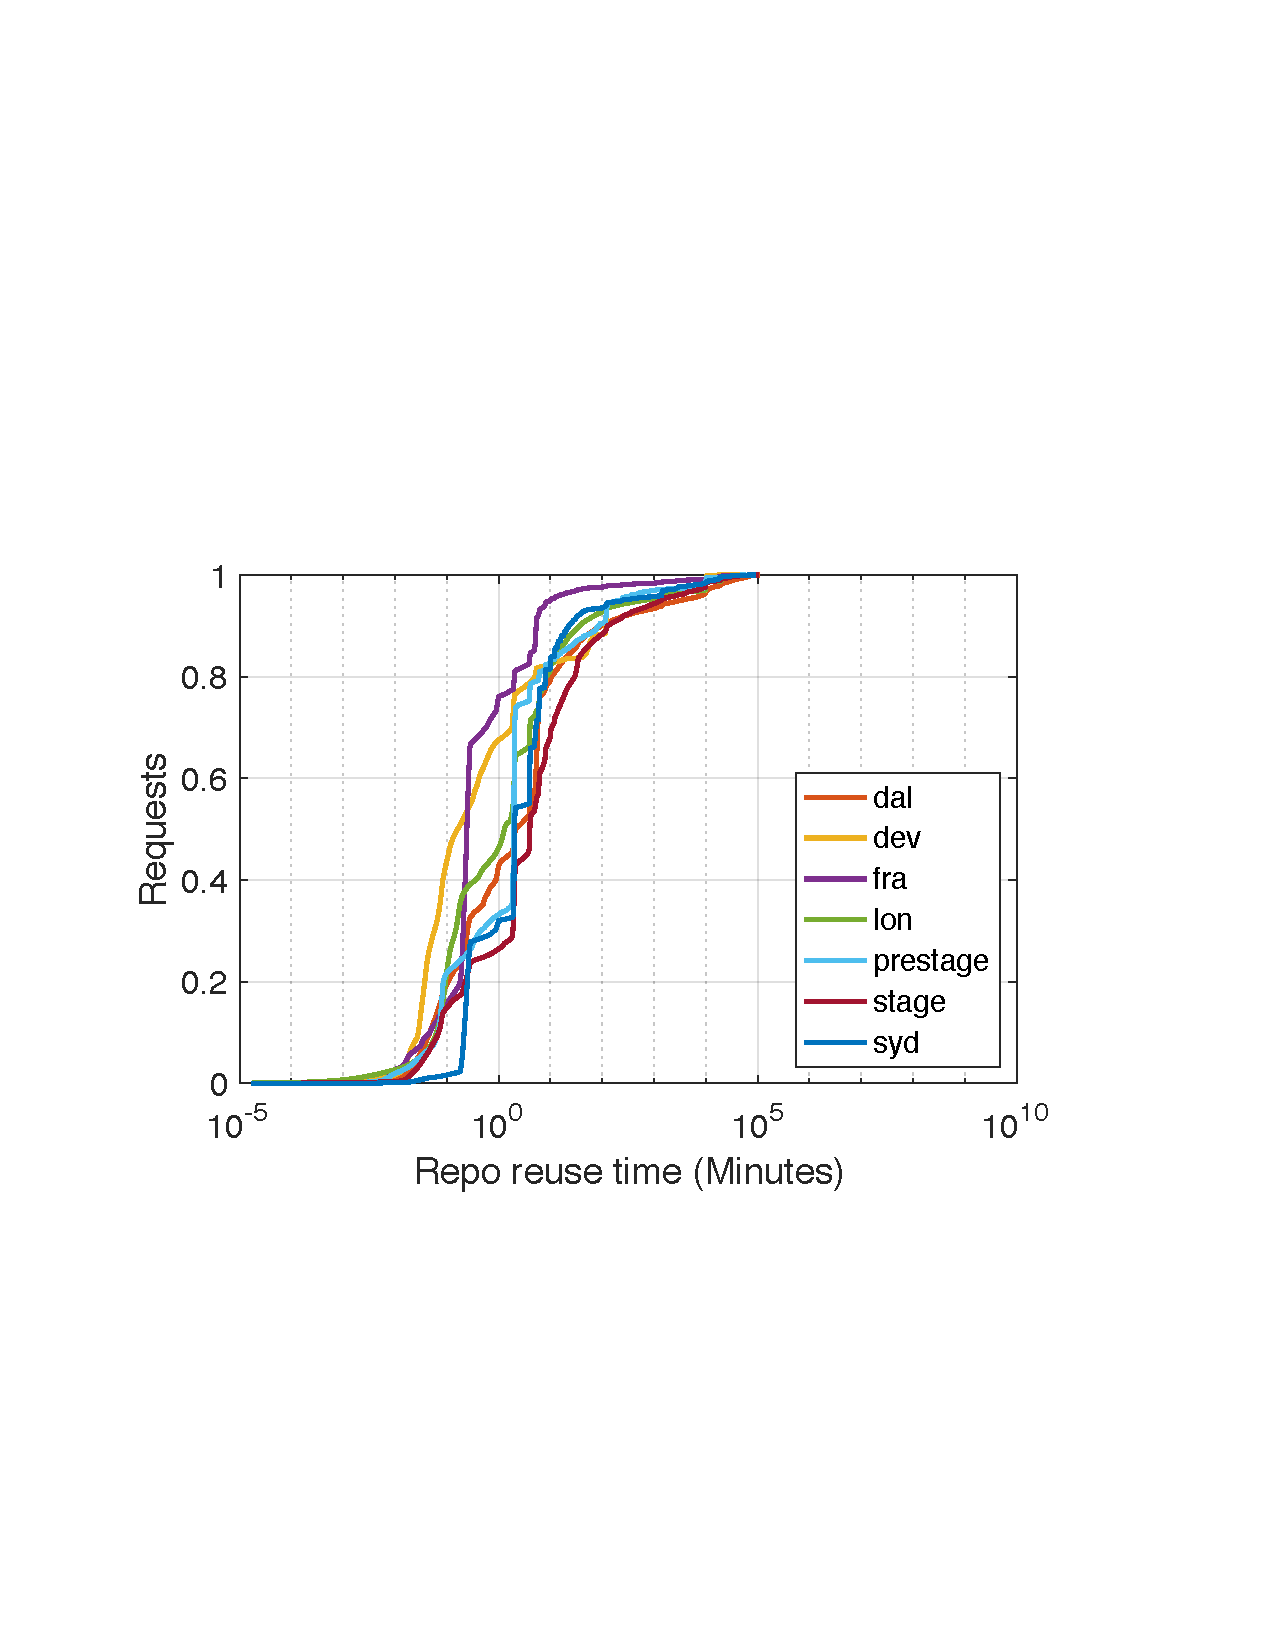
\includegraphics[width=0.2\linewidth]{graphs/repo-reusetime.pdf}
%				\label{fig:repo-reuse}
%	}
%	\subfigure[Client repulling probability]{
%		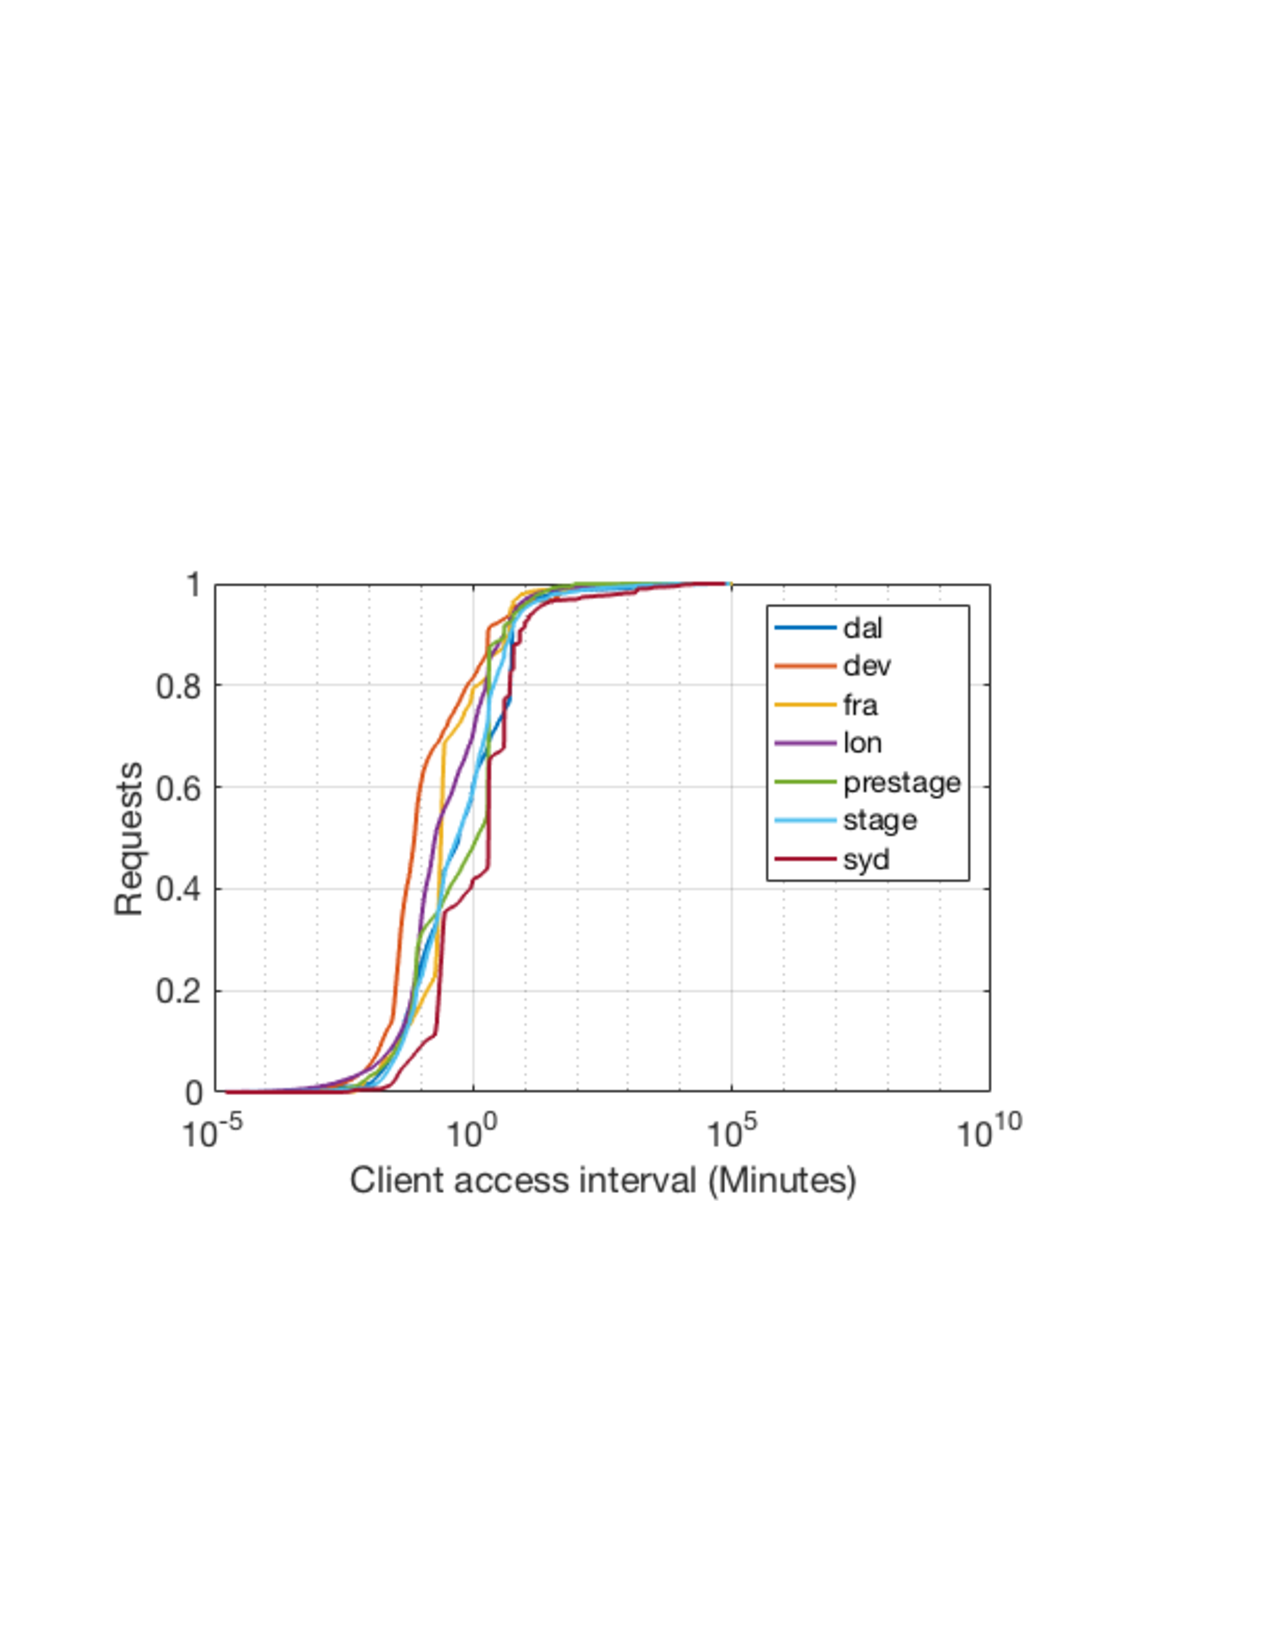
\includegraphics[width=0.2\linewidth]{graphs/user-intervals.pdf}
%			\label{fig:user-interval}
%	}
%	\caption{CDF of reusetime for layers, repositories and clients' access intervals.}
%	\label{fig:fig-reuse}
%\end{figure*}

%\begin{figure}[t]
%	\centering
%	\begin{minipage}{0.26\textwidth}
%		\centering
%		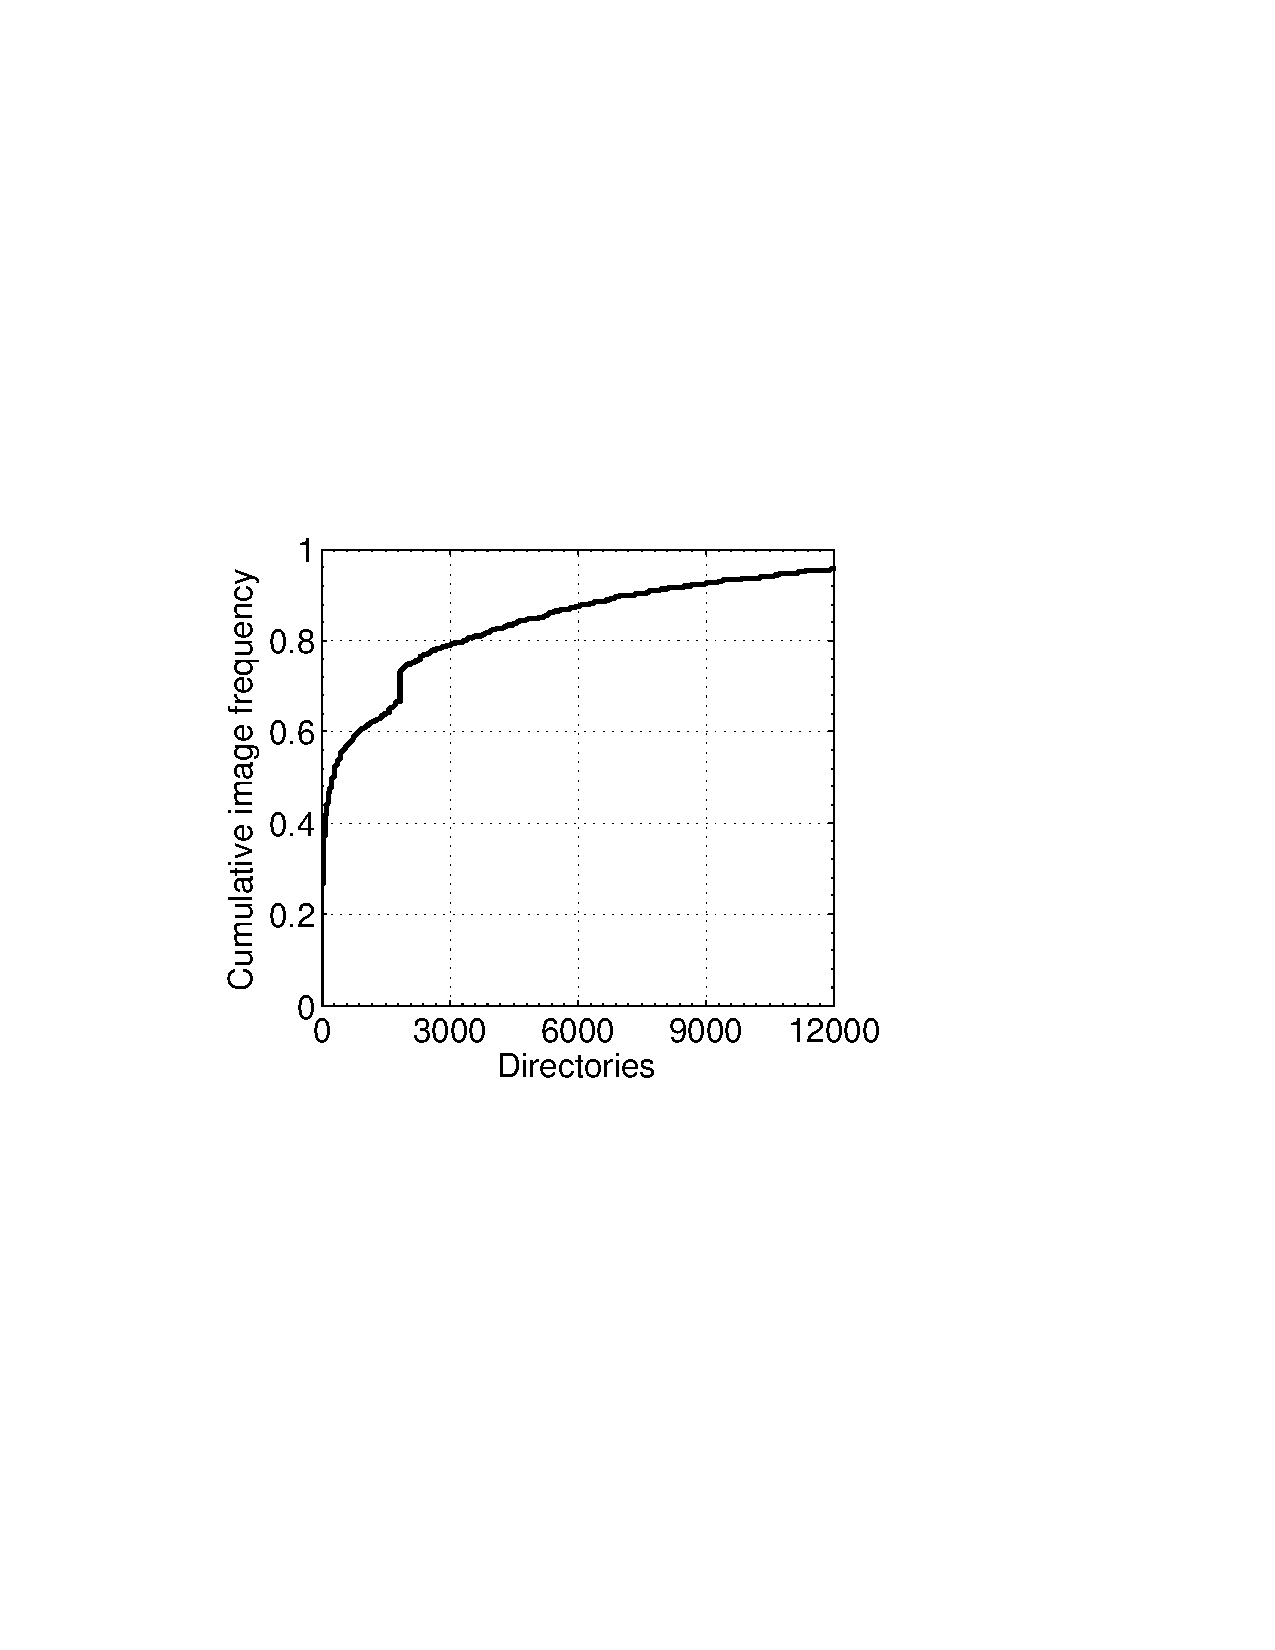
\includegraphics[width=1\textwidth]{graphs/dir.pdf}
%		\caption{CDF of images by\newline directories}
%		\label{fig-dir}
%	\end{minipage}%
%	\begin{minipage}{0.24\textwidth}
%		\centering
%		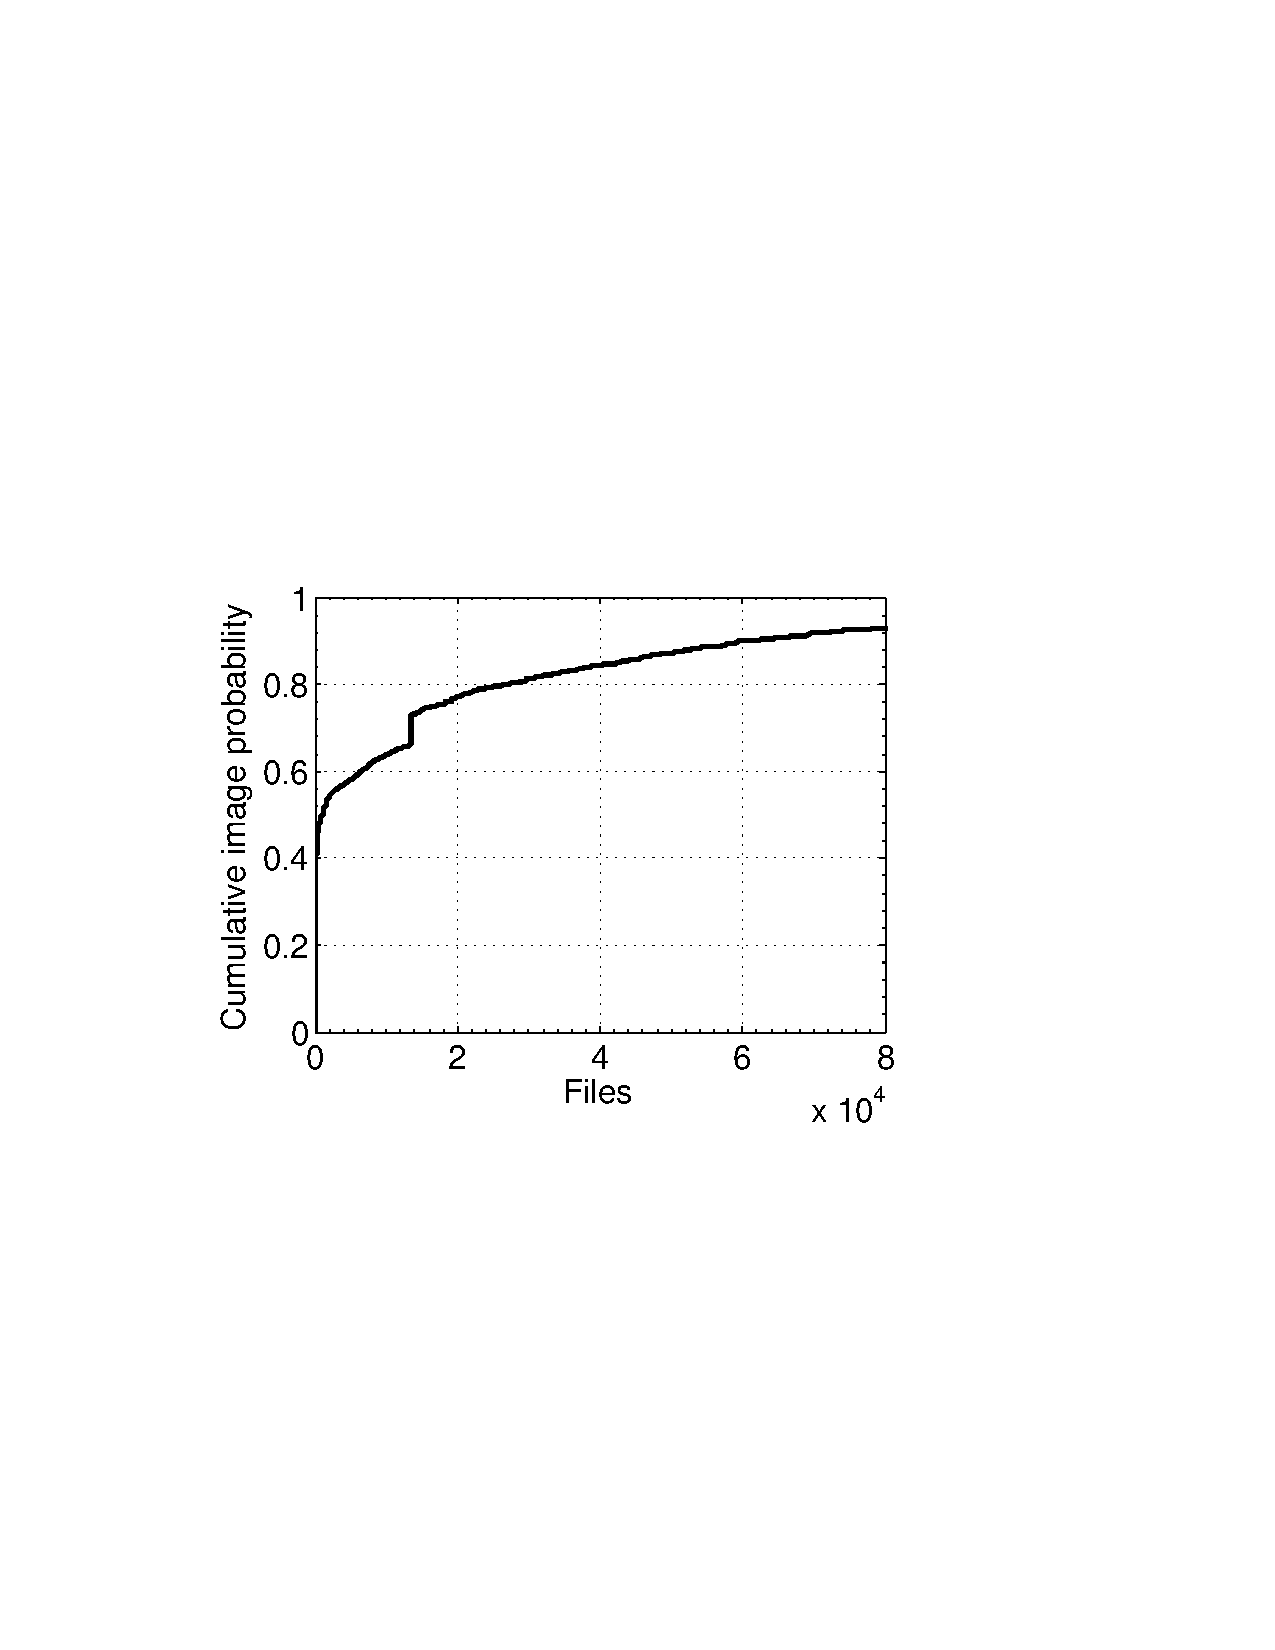
\includegraphics[width=1\textwidth]{graphs/file.pdf}
%		\caption{CDF of images by files}
%		\label{fig-file}
%	\end{minipage}
%\end{figure}

%\begin{figure}[htbp] 
%	\begin{minipage}{0.5\linewidth} 
%		\centering 
%		\includegraphics{circle} 
%		\caption{A Circle} 
%		\label{fig:circle} 
%	\end{minipage}% 
%	\begin{minipage}{0.5\linewidth} 
%		\centering 
%		\includegraphics{rectangle} 
%		\caption{A Rectangle} 
%		\label{fig:rectangle} 
%	\end{minipage} 
%\end{figure}
%
%As shown in~\cite{xxx},
%layer accesses are heavy skewed.
%There are hot layers that account for majority of layer accesses. 
%Hence, we can cache hot layers to improve performance.
Is it possible to 
preconstruct a layer before users pull a layer to save layer restoring latency?
We analyze the duration between a \texttt{pulling} manifest request and the subsequent \texttt{pulling} layer requests
and show in Figure~\ref{fig:intervals}.
We see that 
majority of intervals are greater than 1 s.
For example, 80\% of intervals from \texttt{lon} are greater than 1 s.
60\% of intervals from \texttt{syd} are greater than 5 s.
Hence,
there is a relatively long gap between a \texttt{pulling} manifest request and the subsequent \texttt{pulling} layer requests.
This is because, first,
when fetching an image from registry,
Docker client \emph{downloads} a certain number layers in parallel (3 by default)
starting from the lowest or base layers.
In this case, if the image contains more than 3 layers, then the \emph{upper} layers have to 
wait til the \emph{lower} layers are downloaded, which varies
\texttt{pulling} layer request arrive time on registry.
Second, network delay between clients and registries 
often accounts for a greater proportion of pulling latency in Cloud environment, especially for
large layers.
Consequently,
we can use this long gap to predict which layers will be pulled by the user
when a \texttt{pulling} manifest request is received,
 and then 
rebuild a layer for the user before \texttt{pulling} layer requests arrive.

%majority of \texttt{pull} layer requests access only few layers.
%\paragraph{Skewness}
%Figure~\ref{fig:layer-skewness} shows the CDF of layer popularity.
%We observe a heavy layer access skewness for \texttt{Fra}, \texttt{Syd}, \texttt{Dal}, \texttt{Stage}, and \texttt{Lon} with 60-80\%  of the \texttt{pull} layer requests accessing only 10\% of layers.
%Figure~\ref{fig:repo-skewness} shows the CDF of repository popularity.
%Compare to layer popularity, 
%repository access skewness is heavier across 7 workloads.
%Almost 90\% of \texttt{pull} layer requests access only 10\% of repositories for 
%\texttt{Dev}, \texttt{Fra}, \texttt{Prestage}, \texttt{Syd}, and \texttt{Stage}.
%Figure~\ref{fig:client-skewness} shows the CDF of client popularity.
%\texttt{Dal}, \texttt{Dev}, \texttt{Fra}, \texttt{Lon}, \texttt{Prestage}, and \texttt{Stage} shows a heavy client access skewness with
%10\% of clients send 95\% \texttt{pull} layer requests for \texttt{Lon}.
%Overall, caching a layer with higher pull count will improve the hit ratio, 
%especially for popular repositories and targeting active clients with higher repulling probability.
%
%\paragraph{Reuse time}
%Next, we analyze the layer and repository reuse time.
%Layer reuse time means the duration between two consecutive requests to the same layer
%while repository reuse time means the duration between two consecutive \emph{pull} manifest requests to the same repository.
%Figure~\ref{fig:layer-reuse} shows the CDF of layer reuse time. 
%%Layer reuse time means the duration between two consecutive \texttt{pull} requests to the same layer.
%We see that layer reuse time distribution varies among different workloads.
%For \texttt{Fra}, \texttt{Syd}, and \texttt{Stage},
%half of the layers' reuse time is shorter than 6 minutes.
%Half of layers from \texttt{Dal} and \texttt{Lon} have a reuse time higher than 1 hour and is higher than 100 hours for \texttt{Prestage} and \texttt{Dev}.
%Consequently, for \texttt{Dal}, \texttt{Lon}, \texttt{Prestage}, and \texttt{Dev}, 
%it may take longer than 1 hour for at least half newly requested layer to get a hit. 
%These layers shouldn't be cached since their reuse time is too long and may cause other useful layers or slices to be evicted, called \emph{cache pollution}.
%%Consider popular skewness, 
%Figure~\ref{fig:repo-reuse} shows the CDF of repository reuse time.
%%Repository reuse time means the duration between two consecutive \texttt{pull manifest} requests to the same repository.
%We see that repository reuse time is much shorter than layer reuse time.
%80\% of repositories are requested within 2-12 minutes across the 7 workloads.
%Figure~\ref{fig:user-interval} shows the CDF of client access intervals.
%client access interval means the duration between two consective requests issued by the same client.
%Client access intervals are much shorter than repository reuse time.
%80\% of client are active within 1 - 3 minutes for the 7 workloads. 
%Hence, to eliminate \emph{cache pollution},
%we consider the reuse time of layer and repository as well as client access intervals during cache eviction.

%<<<<<<< HEAD
%=======
%\paragraph{Skewness.}
%Figure~\ref{fig:layer-skewness} shows the CDF of layer popularity.
%We observe a heavy layer access skewness for \texttt{Fra}, \texttt{Syd}, \texttt{Dal}, \texttt{Stage}, and \texttt{Lon} workloads with $60$-$80$\%  of the \texttt{pull} layer requests accessing only $10$\% of the layers.
%Figure~\ref{fig:repo-skewness} shows the CDF of repository popularity.
%Compared to layer popularity, 
%repository access skewness is heavier across all the 7 workloads.
%Almost $9$\% of \texttt{pull} layer requests access only $10$\% of repositories for 
%\texttt{Dev}, \texttt{Fra}, \texttt{Prestage}, \texttt{Syd}, and \texttt{Stage}.
%Figure~\ref{fig:client-skewness} shows the CDF of client popularity.
%\texttt{Dal}, \texttt{Dev}, \texttt{Fra}, \texttt{Lon}, \texttt{Prestage}, and \texttt{Stage} show a heavy client access skewness. 
%For example, only $10$\% of clients issue $95$\% of the \texttt{pull} layer requests in the \texttt{Lon} workload.
%Therefore, caching a layer with a high pull count will improve the hit ratio, 
%especially for popular repositories and targeting active clients with high repulling probability.
%
%\paragraph{Reuse time.}
%Next, we analyze the layer and repository reuse time.
%Layer reuse time means the duration between two consecutive requests to the same layer
%while repository reuse time means the duration between two consecutive \emph{pull} manifest requests to the same repository.
%Figure~\ref{fig:layer-reuse} shows the CDF of layer reuse time. 
%%Layer reuse time means the duration between two consecutive \texttt{pull} requests to the same layer.
%We see that layer reuse time distribution varies among different workloads.
%For \texttt{Fra}, \texttt{Syd}, and \texttt{Stage},
%half of the layers' reuse time is shorter than $6$ minutes.
%Half of layers from \texttt{Dal} and \texttt{Lon} have a reuse time higher than $1$ hour and it is higher than $100$ hours for \texttt{Prestage} and \texttt{Dev}.
%Consequently, for \texttt{Dal}, \texttt{Lon}, \texttt{Prestage}, and \texttt{Dev}, 
%it may take longer than $1$ hour for at least half newly requested layers to get a hit. 
%These layers should not be cached since their reuse time is too long and may cause other useful layers or slices to be evicted, \ie causing \emph{cache pollution}.
%%Consider popular skewness, 
%Figure~\ref{fig:repo-reuse} shows the CDF of repository reuse time.
%%Repository reuse time means the duration between two consecutive \texttt{pull manifest} requests to the same repository.
%We see that repository reuse time is much shorter than layer reuse time.
%$80$\% of repositories are requested within $2$-$12$ minutes across all the 7 workloads.
%Figure~\ref{fig:user-interval} shows the CDF of client access intervals.
%client access interval refers to the duration between two consecutive requests issued by the same client.
%Client access intervals are much shorter than repository reuse time.
%$80$\% of client are active within $1$-$3$ minutes for the 7 workloads. 
%Hence, to eliminate cache pollution,
%we consider both the reuse time of layer and repository as well as client access intervals during cache eviction.
%
%\subsection{Layer Deduplication}
%
%\paragraph{Redundant files shared among layers.}
%Consider that deduplication incurs a performance overhead and the current Docker registry already stores layers in compressed format to save space and network transfer overhead. We first analyze the space efficiency of a registry that performs decompression and file-level deduplication and compare it to a registry that naively stores compressed layers.
%
%In Figure~\ref{fig:cacheefficiency}, the x-axis values correspond to the sizes of 5 samples of registry data of varying sizes with traditional layer compression. For a traditional registry, the compressed layer tarballs will be kept as is.
%While a registry with file-level deduplication will store \emph{deduplicated} layers (i.e., unique files). 
%The y-axis shows how much space a registry with file-level deduplication can save over compressed layer tarballs.
%For the first two samples of the dataset, with size less than $20$~GB, 
%there is no benefit to \emph{deduplicate} layers because the deduplication ratio is very low.
%However, when the dataset size is $200$~GB and over, we can save over $40$\% of space. Saved space increases almost linearly with the size of the layer dataset.
%This affirms the benefit of deduplicating layers as the registry size increases.
%
%\paragraph{Layer preconstruction.}
%>>>>>>> 94daa3df1d5d977ac11fd9da2aea7b4eed340be2
%\subsubsection{User access pattern based preconstruction}
%
%Docker client stores images as lists of layers and layers are shared among different repositories, 
%which is similar to Docker registry.
%When a client pulls an image from a repository, 
%it will first \texttt{pull} the manifest of the image~\cite{docker}~\cite{dockerworkload} and 
%parse the manifest to get the layer digests,
%then lookup each layer digest against a \emph{local layer index}.
%After that it only pulls the layers that have \emph{not been stored locally}.
%Theoretically, clients only pull layer once. 
%However, some clients may delete several local images and \emph{repull} layers for these images.
%%Moreover, kubernetes allows users always \emph{repull} layers no matter these layers locally available or not~\cite{docker}.  
%Here, a \emph{repull layer} indicates a layer a user pulls multiple times,
%and a \emph{non-repull layer} means users only pull this layer once.
%
%\preconstructcachename~starts parallel slice restoring for layers 
%when a \texttt{pull manifest} request is received, 
%which is called layer preconstruction.
%These preconstructed layer slices are temporally stored in the cache for later \texttt{pull slice} requests.
%In this case, slice restoring process and its overhead can be avoided if the requested slice is found in the cache.
%Next, we analyze user access patterns to identify which layers in the repository will be pulled by users after 
%\texttt{pull manifest} requests.



%\paragraph{Monitor user access patterns}
%To monitor user access patterns,
%\preconstructcachename~first uses a RLmap to record repository-layer relationship.
%If user~\emph{u} \emph{pushes} a  layer~\emph{l} to a repository~\emph{r},
%\preconstructcachename~will add an new entry (\emph{l}) in RLmap denoted as RLmap[\emph{r, l}]. 
%%Based on user access patterns,
%\preconstructcachename~ also maintains a URLmap for keeping track of user access patterns.
%To identify a user, 
%we extract \emph{user end host address} (\emph{r.client}) from each request (\emph{r}). 
%Each URLmap entry maintains a user profile for each user \emph{u} denoted as URLmap[\emph{u}]. %as shown in Figure~\ref{xxx}.
%User profile contains a list of repository profiles for each accessed repository \emph{repo} denoted as URLmap[\emph{u, repo}],
%and each repo profile contains a list of layer profiles for each accessed layer \emph{l}  denoted as URLmap[\emph{u, repo, l}].
%Note that layer profiles can be shared among different repo profiles for the same user.
%If user~\emph{u} \texttt{pull}s a layer~\emph{l} from a repository~\emph{repo},
%\preconstructcachename will update layer profile URLmap[\emph{u, repo, l}] with the corresponding layer repull count, and calculate
%repository repulling probability and user repulling probability for the corresponding repository profile and user profile.
%Each node records the following history information: (\emph{Get\_cnt}, \emph{Put\_cnt}, \emph{last\_access\_time}). a child node layer~\emph{L} to parent node~\emph{R}
%User profile records the user repulling probability $u.rp$ for client $u$.
%If $u.rp$ is greater than threshold $\theta_{crp}$, this user has a high probability of repulling layers.
%Repo profile records repository repulling probability $u.r.rp$ for repository $r$.
%If $u.r.rp$ is greater than threshold $\theta_{rrp}$, this repository is a popular repulling repository for this user.
%Layer profile records layer repull count $u.l.R$ for layer $l$.
%If $u.l.R$ is greater than threshold $\theta_{R}$, this layer is a popular repull layer for this user.



%\subsubsection{User access pattern  based cache replacement}

%
%\preconstructcachename~starts cache eviction when free space is low.
%To decide which layer or slices need to be evicted to make space for new requests,
%we analyze the temporal trend of user accesses as follows.

